\part{Spatial Data}
\label{cha:Spatial}

\chapter{Displaying Spatial Data: Introduction}
\label{cha:spatialIntro}

Spatial data (also known as geospatial data) are directly or
indirectly referenced to a location on the surface of the Earth. Their
spatial reference is composed of coordinate values and a system of
reference for these coordinates. Spatial data are often accessed,
manipulated, or analyzed through Geographic Information Systems (GIS).

Real objects represented by GIS data can be divided into two
abstractions: discrete objects (e.g., a road or a river)
represented with vector data (points, lines, and polygons), and
continuous fields (such as elevation or solar radiation)
represented with raster data. The \texttt{sp} package is the
preferred option to use vector data in \textsf{R}, and the
\texttt{raster} package is the choice for raster
data\footnote{Although \texttt{sp} and \texttt{raster} are the
  most important packages, there are an increasing number of
  packages designed to work with spatial data. They are summarized
  in the corresponding CRAN Task View. Read Section
  \ref{cha:further-reading-spatial} for details.}.

This part exposes several examples where vector and raster data
are displayed to show geographic location of features and physical
landscape features of a place (reference and physical maps,
Chapter \ref{cha:refer-phys-maps}) or a specific variable in the
context of a geographic reference (thematic maps, Chapter
\ref{cha:thematicMaps}). These examples make use of several datasets
(available at the book website) described in Chapter
\ref{cha:dataSpatial}.


\section{Packages}
\label{sec:spatial-packages}

The CRAN Tasks View ``Analysis of Spatial
Data''\footnote{\url{http://CRAN.R-project.org/view=Spatial}}
summarizes the packages for reading, vizualizing, and analyzing
spatial data. This section provides a brief introduction to
\texttt{sp}, \texttt{raster}, \texttt{rasterVis}, \texttt{maptools},
\texttt{rgdal}, \texttt{gstat}, and \texttt{maps}. Most of the
information has been extracted from their vignettes, webpages, and help
pages. You should read them for detailed information.

\subsection{sp}
\label{sec:sp}

\index{Packages!sp@\texttt{sp}}

The \texttt{sp} package \cite{Pebesma.Bivand2005} provides classes and
methods for dealing with spatial data in \textsf{R}. The spatial data
classes implemented are points (\texttt{SpatialPoints}), grids
(\texttt{SpatialPixels} and \texttt{SpatialGrid}), lines
(\texttt{Line}, \texttt{Lines} and \texttt{SpatialLines}), rings, and
polygons (\texttt{Polygon}, \texttt{Polygons}, and
\texttt{SpatialPolygons}), each of them without data or with data (for
example, \texttt{SpatialPointsDataFrame} or
\texttt{SpatialLinesDataFrame}).

Selecting, retrieving, or replacing certain attributes in spatial
objects with data is done using standard methods:
\begin{itemize}
\item \texttt{[} selects rows (items) and columns in the
  \texttt{data.frame}.
\item \texttt{[[} selects a column from the \texttt{data.frame}
\item \texttt{[[<-} assigns or replaces values to a column in the
  \texttt{data.frame}.
\end{itemize}

A number of spatial methods are available for the classes in \texttt{sp}:
\begin{itemize}
\item \texttt{coordinates(object) <- value} sets spatial coordinates
  to create spatial data. It promotes a \texttt{data.frame} into a
  \texttt{SpatialPointsDataFrame}. \emph{value} may be specified by a
  formula, a character vector, or a numeric matrix or
  \texttt{data.frame} with the actual coordinates.
\item \texttt{coordinates(object, ...)} returns a matrix with the
  spatial coordinates. If used with \texttt{SpatialPolygons} it
  returns a matrix with the centroids of the polygons.
\item \texttt{bbox} returns a matrix with the coordinates bounding
  box.
\item \texttt{proj4string(object)} and \texttt{proj4string(object) <-
    value} retrieve or set projection attributes on spatial classes.
\item \texttt{spTransform} transforms from one coordinate reference
  system (geographic projection) to another (requires package
  \texttt{rgdal}).
\item \texttt{spplot} plots attributes combined with spatial data:
  Points, lines, grids, polygons.
\end{itemize}

\subsection{raster}
\label{sec:raster}

\index{Packages!raster@\texttt{raster}}

The \texttt{raster} package \cite{Hijmans2013} has functions for
creating, reading, manipulating, and writing raster data. The package
provides general raster data manipulation functions. The package also
implements raster algebra and most functions for raster data
manipulation that are common in Geographic Information Systems (GIS).

The raster package can work with raster datasets stored on disk if
they are too large to be loaded into memory. The package can work with
large files because the objects it creates from these files only
contain information about the structure of the data, such as the
number of rows and columns, the spatial extent, and the filename, but
it does not attempt to read all the cell values in memory. In
computations with these objects, the data are processed in chunks.

The package defines a number of \texttt{S4}
classes. \texttt{RasterLayer}, \texttt{RasterBrick}, and
\texttt{RasterStack} are the most important:
\begin{itemize}
\item A \texttt{RasterLayer} object represents single-layer (variable)
  raster data. It can be created with the function
  \texttt{raster}. This function is able to create a
  \texttt{RasterLayer} from another object, including another
  \texttt{Raster*} object, or from a \texttt{SpatialPixels*} and
  \texttt{SpatialGrid*} object, or even a matrix. In addition, it can
  create a \texttt{RasterLayer} reading data from a file. The
  \texttt{raster} package can use raster files in several formats,
  some of them via the \texttt{rgdal} package. Supported formats for
  reading include GeoTIFF, ESRI, ENVI, and ERDAS.

\item \texttt{RasterBrick} and \texttt{RasterStack} are classes for
  multilayer data. A \texttt{RasterStack} is a list of
  \texttt{RasterLayer} objects with the same spatial extent and
  resolution. It can be formed with a collection of files in different
  locations or even mixed with \texttt{RasterLayer} objects that only
  exist in memory.  A \texttt{RasterBrick} is truly a multilayered
  object, and processing it can be more efficient than processing a
  \texttt{RasterStack} representing the same data.

\end{itemize}

The \texttt{raster} package defines a number of methods for raster
algebra with \texttt{Raster*} objects: arithmetic operators, logical
operators, and functions such as \texttt{abs}, \texttt{round},
\texttt{ceiling}, \texttt{floor}, \texttt{trunc}, \texttt{sqrt},
\texttt{log}, \texttt{log10}, \texttt{exp}, \texttt{cos},
\texttt{sin}, \texttt{max}, \texttt{min}, \texttt{range},
\texttt{prod}, \texttt{sum}, \texttt{any}, and \texttt{all}. In these
functions, \texttt{Raster*} objects can be mixed with numbers.

There are several functions to modify the content or the spatial
extent of \texttt{Raster*} objects, or to combine \texttt{Raster*}
objects:
\begin{itemize}
\item The \texttt{crop} function takes a geographic subset of a larger
  \texttt{Raster*} object. \texttt{trim} crops a \texttt{RasterLayer}
  by removing the outer rows and columns that only contain \texttt{NA}
  values. \texttt{extend} adds new rows and/or columns with
  \texttt{NA} values.
\item The \texttt{merge} function merges two or more \texttt{Raster*}
  objects into a single new object.
\item \texttt{projectRaster} transforms values of a \texttt{Raster*}
  object to a new object with a different coordinate reference system.
\item With \texttt{overlay}, multiple \texttt{Raster*} objects can be
  combined (for example, multiply them).
\item \texttt{mask} removes all values from one layer that are
  \texttt{NA} in another layer, and \texttt{cover} combines two layers
  by taking the values of the first layer except where these are
  \texttt{NA}.
\item \texttt{calc} computes a function for a \texttt{Raster*}
  object. With \texttt{RasterLayer} objects, another
  \texttt{RasterLayer} is returned. With multilayer objects the result
  depends on the function: With a summary function (\texttt{sum},
  \texttt{max}, etc.),  \texttt{calc} returns a \texttt{RasterLayer}
  object, and a \texttt{RasterBrick} object otherwise.
\item \texttt{stackApply} computes summary layers for subsets of a
  \texttt{RasterStack} or \texttt{RasterBrick}.
\item \texttt{cut} and \texttt{reclassify} replace ranges of values
  with single values.
\item \texttt{zonal} computes zonal statistics, that is, summarizes a
  \texttt{Raster*} object using zones (areas with the same integer
  number) defined by another \texttt{RasterLayer}.
\end{itemize}


\subsection{rasterVis}
\label{sec:rasterVis}
\index{Packages!rasterVis@\texttt{rasterVis}}

The \texttt{rasterVis} package \cite{Perpinan.Hijmans2013} complements
the \texttt{raster} package, providing a set of methods for enhanced
visualization and interaction. This package defines visualization
methods (\texttt{levelplot}) for quantitative data and categorical
data, both for univariate and multivariate rasters.

It also includes several methods in the frame of the Exploratory Data
Analysis approach: scatterplots with \texttt{xyplot}, histograms and
density plots with \texttt{histogram} and \texttt{densityplot}, violin
and boxplots with \texttt{bwplot}, and a matrix of scatterplots with
\texttt{splom}.

On the other hand, this package is able to display vector fields using
arrows, \texttt{vectorplot}, or with streamlines
\cite{Wegenkittl.Groeller1997}, \texttt{streamplot}. In this last
method, for each point, \emph{droplet}, of a jittered regular grid, a
short streamline portion, \emph{streamlet}, is calculated by
integrating the underlying vector field at that point. The main color
of each streamlet indicates local vector magnitude (slope). Streamlets
are composed of points whose sizes, positions, and color degradation
encode the local vector direction (aspect).


\subsection{maptools}
\label{sec:maptools}
\index{Packages!maptools@\texttt{maptools}}

The \texttt{maptools} package \cite{Bivand.Lewin-Koh2013} provides a
set of tools for manipulating and reading geographic data, in
particular ESRI (Environmental Systems Research Institute)
shapefiles. The package also provides interface wrappers for
exchanging spatial objects with packages such as PBSmapping, spatstat,
maps, RArcInfo, Stata tmap, WinBUGS, Mondrian, and others. The main
functions in the context of this book are

\begin{itemize}

\item \texttt{readShapePoints} reads data from a points shapefile into
  a \texttt{SpatialPointsDataFrame} object.

\item \texttt{writePointsShape} writes data from a
  \texttt{SpatialPointsDataFrame} object to a shapefile.

\item \texttt{readShapeLines} reads data from a line shapefile
  into a \texttt{SpatialLinesDataFrame} object.

\item \texttt{writeLinesShape} writes data from a
  \texttt{SpatialLinesDataFrame} object to a shapefile.

\item \texttt{readShapePoly} reads data from a polygon shapefile into
  a \texttt{SpatialPolygonsDataFrame} object.

\item \texttt{writePolyShape} writes data from a
  \texttt{SpatialPolygonsDataFrame} object to a shapefile.

\item \texttt{map2SpatialPolygons} and \texttt{map2SpatialLines} may
  be used to convert map objects returned by the \texttt{map} function
  in the \texttt{maps} package to the classes defined in the
  \texttt{sp} package.

\item \texttt{spCbind} provides cbind-like methods for
  \texttt{Spatial*DataFrame} and \texttt{data.frame} objects.
 
\end{itemize}

The topology operations on geometries performed by this package (for
example, \texttt{unionSpatialPolygons} ) use the package
\texttt{rgeos}, an interface to the Geometry Engine Open Source
(GEOS)\footnote{\url{http://trac.osgeo.org/geos/}}.


\subsection{rgdal}
\label{sec:rgdal}
\index{Packages!rgdal@\texttt{rgdal}}

The \texttt{rgdal} package \cite{Bivand.Keitt.ea2013} provides
bindings to the Geospatial Data Abstraction Library
(GDAL)\footnote{\url{http://www.gdal.org/}}. With \texttt{readOGR} and
\texttt{readGDAL}, both GDAL raster and OGR vector map data can be
imported into \textsf{R}, and GDAL raster data and OGR vector data can
be exported with \texttt{writeGDAL} and \texttt{writeOGR}.

In addition, this package provides access to projection and
transformation operations from the PROJ.4
library\footnote{\url{https://trac.osgeo.org/proj/}}. This package
implements several \texttt{spTransform} methods providing
transformation between datums and conversion between projections using
PROJ.4 projection arguments.


\subsection{gstat}
\label{sec:gstat}
\index{Packages!gstat@\texttt{gstat}}

The \texttt{gstat} package \cite{Pebesma2004} provides functions for
geostatistical modeling, prediction, and simulation, including
variogram modeling and simple, ordinary, universal, and external drift
kriging.

Most of the functionality of this package is beyond the scope of this
book. However, some functions must be mentioned:
\begin{itemize}
\item \texttt{variogram} calculates the sample variogram from data, or
  for the residuals if a linear model is given. \texttt{vgm} generates
  a variogram and \texttt{fit.variogram} fit ranges and/or sills from
  a variogram model to a sample variogram.
\item \texttt{krige} is the function for simple, ordinary or universal
  kriging. \texttt{gstat} is the function for univariate or
  multivariate geostatistical prediction.
\end{itemize}

\subsection{maps}
\label{sec:maps}
\index{Packages!maps@\texttt{maps}}
\index{Packages!mapproj@\texttt{mapproj}}
\index{Packages!mapdata@\texttt{mapdata}}

The \texttt{maps} \cite{Becker.Wilks.ea2013}, \texttt{mapdata}
\cite{Becker.Wilks.ea2013b}, and \texttt{mapproj}
\cite{McIlroy.Brownrigg.ea2013} packages are useful to draw or create
geographical maps. \texttt{mapdata} contains higher resolution
databases, and \texttt{mapproj} converts latitude/longitude
coordinates into projected coordinates.


\section{Further Reading}
\label{cha:further-reading-spatial}

\begin{itemize}

\item \cite{Slocum.McMaster.ea2005} and \cite{Dent.Torguson.ea2008}
  are comprehensive books on thematic cartography and
  geovisualization. They include chapters devoted to data
  classification, scales, map projections, color theory, typography,
  and proportional symbol, choropleth, dasymetric, isarithmic, and
  multivariate mapping. Several resources are available at their
  accompanying
  websites\footnote{\url{http://www.pearsonhighered.com/slocum3e/} and
    \url{http://highered.mcgraw-hill.com/sites/0072943823/}}.

\item \cite{Bivand.Pebesma.ea2008} is the essential reference to work
  with spatial data in \textsf{R}. R. Bivand and E. Pebesma are the
  authors of the fundamental \texttt{sp} package, and they are the
  authors or maintainers of several important packages such as
  \texttt{gstat}, for geostatistical modeling, prediction, and
  simulation, \texttt{rgdal}, \texttt{rgeos} and
  \texttt{maptools}. Chapter 3 is devoted to the visualization of
  spatial data. Code, figures, and data of the book are available at
  the accompanying website\footnote{\url{http://www.asdar-book.org/}}.

\item \cite{Hengl2009} is an open-access book with seven spatial
  data analysis exercises. The author is the creator and
  maintainer of the Spatial-Analyst
  webpage\footnote{\url{http://spatial-analyst.net}}.

\item The CRAN Tasks View ``Analysis of Spatial
  Data''\footnote{\url{http://CRAN.R-project.org/view=Spatial}}
  summarizes the packages for reading, vizualizing, and analyzing
  spatial data.  The packages in development published at R-Forge are
  listed in the ``Spatial Data \& Statistics'' topic
  view\footnote{\url{http://r-forge.r-project.org/softwaremap/trove_list.php?form_cat=353}}.
  The R-SIG-Geo mailing
  list\footnote{\url{https://stat.ethz.ch/mailman/listinfo/R-SIG-Geo/}}
  is a powerful resource for obtaining help.

\item The ``Spatial
  Analysis''\footnote{\url{http://spatialanalysis.co.uk/map-gallery/}}
  and ``Kartograph''\footnote{\url{http://kartograph.org/}} webpages
  publish a variety of beautiful visualization examples.

\end{itemize}


\chapter{Thematic Maps}
\label{cha:thematicMaps}

A thematic map focuses on a specific theme or variable, commonly using
geographic data such as coastlines, boundaries, and places as points
of reference for the variable being mapped. These maps provide
specific information about particular locations or areas (proportional
symbol mapping and choropleth maps) and information about spatial
patterns (isarithmic and raster maps). The following sections illustrate
the \textsf{R} code you need to produce these maps, with a final
section devoted to the visualization of vector fields.



\section{Proportional Symbol Mapping}
\label{sec:org50569e0}
\label{sec:bubble}
\subsection{Introduction}
\label{sec:org5c481d2}
The proportional symbol technique uses symbols of different sizes
to represent data associated with areas or point locations, with
circles being the most frequently used geometric symbol. The data
and the size of symbols can be related through different types of
scaling: mathematical scaling sizes areas of point symbols in
direct proportion to the data; perceptual scaling corrects the
mathematical scaling to account for visual understimation of
larger symbols; and range grading, where data are grouped, and each
class is represented with a single symbol size. 

In this chapter we display data from a grid of sensors belonging to
the Integrated Air Quality system of the Madrid City Council (Section
\ref{sec:airQualityData}) with circles as the proportional symbol, and
range grading as the scaling method. The objective when using range
grading is to discriminate between classes instead of estimating an
exact value from a perceived symbol size. However, because human
perception of symbol size is limited, it is always recommended to
add a second perception channel to improve the discrimination
task. Colors from a sequential palette will complement symbol size to
encode the groups.


\subsection{Proportional Symbol with \texttt{spplot}}
\label{sec:org738a6b2}
The \texttt{NO2sp} \texttt{SpatialPointsDataFrame} can be easily displayed
with the \texttt{spplot} method provided by the \texttt{sp} package, based on
\texttt{xyplot} from the \texttt{lattice} package. Both color and size can be
combined in a unique graphical output because \texttt{spplot} accepts
both of them (Figure \ref{fig:airMadrid_spplot}). I define a
sequential palette whose colors denote the value of the variable
(green for lower values of the contaminant, brown for intermediate
values, and black for highest values).

\lstset{language=r,label= ,caption= ,captionpos=b,numbers=none}
\begin{lstlisting}
  library(sp)
  
  load('data/NO2sp.RData')
\end{lstlisting}

\lstset{language=r,label= ,caption= ,captionpos=b,numbers=none}
\begin{lstlisting}
  airPal <- colorRampPalette(c('springgreen1', 'sienna3', 'gray5'))(5)
  
  spplot(NO2sp["mean"], col.regions=airPal, cex=sqrt(1:5),
         edge.col='black', scales=list(draw=TRUE),
         key.space='right')
\end{lstlisting}

\begin{figure}[htbp]
\centering
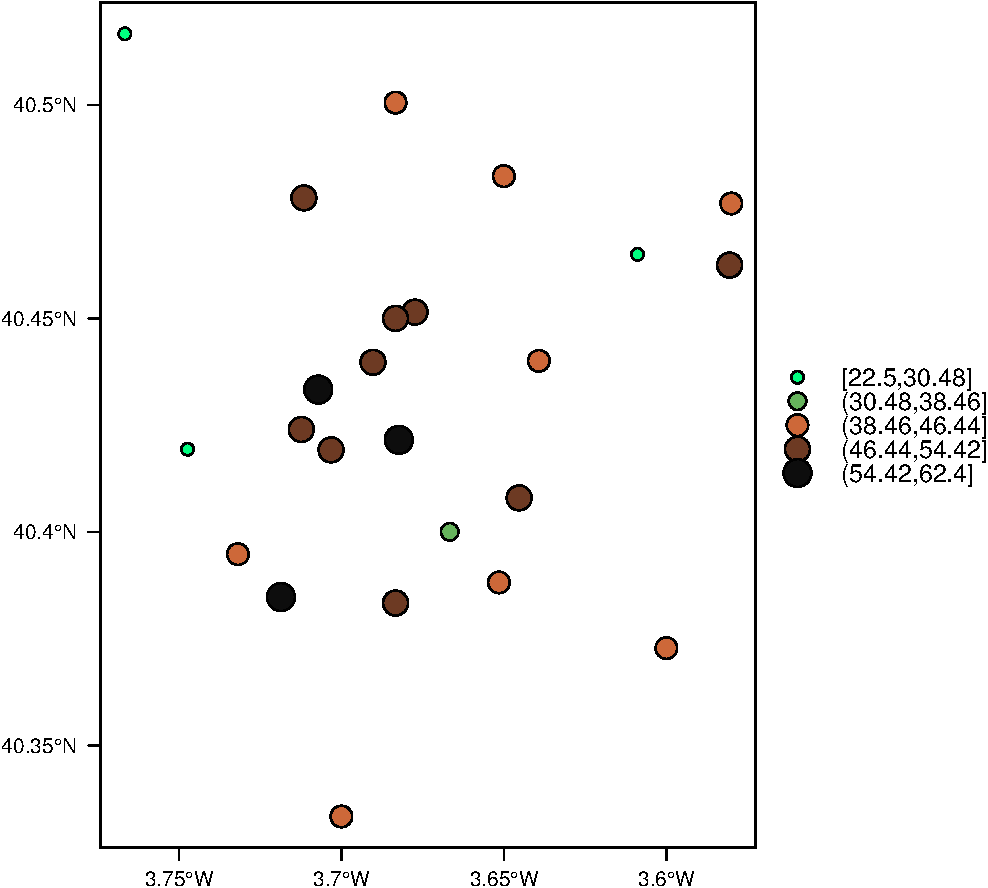
\includegraphics[width=.9\linewidth]{figs/airMadrid_spplot.pdf}
\caption{\label{fig:orgfd87f1f}
Annual average of \(NO_2\) measurements in Madrid. Values are shown with different symbol sizes and  colors for each class with the \texttt{spplot} function.}
\end{figure}

The \texttt{ggplot2} version of this code needs to transform the
\texttt{SpatialPointsDataFrame} to a conventional \texttt{data.frame} (which
will contain two columns with latitude and longitude values).
\lstset{language=r,label= ,caption= ,captionpos=b,numbers=none}
\begin{lstlisting}
  NO2df <- data.frame(NO2sp)
  NO2df$Mean <- cut(NO2sp$mean, 5)
  
  ggplot(data=NO2df, aes(long, lat, size=Mean, fill=Mean)) +
      geom_point(pch=21, col='black') + theme_bw() +
      scale_fill_manual(values=airPal)
\end{lstlisting}

\subsection{Optimal Classification and Sizes to Improve Discrimination}
\label{sec:org0e2a31c}
Two main improvements can be added to Figure
\ref{fig:airMadrid_spplot}:

\begin{itemize}
\item Define classes dependent on the data structure (instead of the
uniform distribution assumed with \texttt{cut}). A suitable approach is
the \texttt{classInterval} function of the \texttt{classInt} package, which
implements the Fisher-Jenks optimal classification
algorithm.
\end{itemize}

\begin{LaTeX}
\index\{Packages!classInt@\texttt{classInt}\}
\index\{classIntervals@\texttt{classIntervals}\}
\index\{findCols@\texttt{findCols}\}
\index\{findColours@\texttt{findColours}\}
\end{LaTeX}

\lstset{language=r,label= ,caption= ,captionpos=b,numbers=none}
\begin{lstlisting}
  library(classInt)
  ## The number of classes is chosen between the Sturges and the
  ## Scott rules.
  nClasses <- 5
  intervals <- classIntervals(NO2sp$mean, n=nClasses, style='fisher')
  ## Number of classes is not always the same as the proposed number
  nClasses <- length(intervals$brks) - 1
\end{lstlisting}

\lstset{language=r,label= ,caption= ,captionpos=b,numbers=none}
\begin{lstlisting}
  op <- options(digits=4)
  tab <- print(intervals)
  options(op)
\end{lstlisting}

\begin{itemize}
\item Encode each group with a symbol size (circle area) such that visual
discrimination among classes is enhanced. The next code uses the set
of radii proposed in \cite{Dent.Torguson.ea2008} (Figure
\ref{fig:dent}). This set of circle sizes is derived from studies by Meihoefer \cite{Meihoefer1969}. He derived a set of ten
circle sizes that were easily and consistently discriminated by his
subjects. The alternative proposed by Dent et al. improves the
discrimination between some of the circles.
\end{itemize}

\lstset{language=r,label= ,caption= ,captionpos=b,numbers=none}
\begin{lstlisting}
  ## Complete Dent set of circle radii (mm)
  dent <- c(0.64, 1.14, 1.65, 2.79, 4.32, 6.22, 9.65, 12.95, 15.11)
  ## Subset for our dataset
  dentAQ <- dent[seq_len(nClasses)]
  ## Link Size and Class: findCols returns the class number of each
  ## point; cex is the vector of sizes for each data point
  idx <- findCols(intervals)
  cexNO2 <- dentAQ[idx]
\end{lstlisting}

\begin{figure}[htbp]
\centering
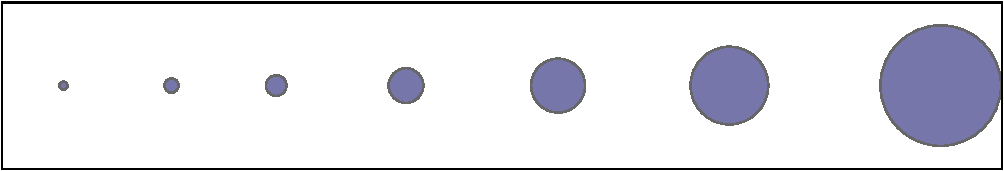
\includegraphics[width=.9\linewidth]{figs/dent.pdf}
\caption{\label{fig:org38bb954}
Symbol sizes proposed by Borden Dent.}
\end{figure}

These two enhancements are included in Figure
\ref{fig:airMadrid_classes}, which displays the categorical variable
\texttt{classNO2} (instead of \texttt{mean}) whose levels are the intervals
previously computed with \texttt{classIntervals}. In addition, this
figure includes an improved legend.

\lstset{language=r,label= ,caption= ,captionpos=b,numbers=none}
\begin{lstlisting}
  NO2sp$classNO2 <- factor(names(tab)[idx])
\end{lstlisting}

\lstset{language=r,label= ,caption= ,captionpos=b,numbers=none}
\begin{lstlisting}
  ## ggplot2 version
  NO2df <- data.frame(NO2sp)
  
  ggplot(data=NO2df, aes(long, lat, size=classNO2, fill=classNO2)) +
      geom_point(pch=21, col='black') + theme_bw() +
      scale_fill_manual(values=airPal) +
      scale_size_manual(values=dentAQ*2)
  
\end{lstlisting}

\lstset{language=r,label= ,caption= ,captionpos=b,numbers=none}
\begin{lstlisting}
  ## spplot version
  
  ## Definition of an improved key with title and background
  NO2key <- list(x=0.98, y=0.02, corner=c(1, 0),
                title=expression(NO[2]~~(paste(mu, plain(g))/m^3)),
                cex.title=.75, cex=0.7,
                background='gray92')
  
  pNO2 <- spplot(NO2sp["classNO2"],
                 col.regions=airPal,  cex=dentAQ,
                 edge.col='black',
                 scales=list(draw=TRUE),
                 key.space=NO2key)
  pNO2
\end{lstlisting}

\begin{figure}[htbp]
\centering
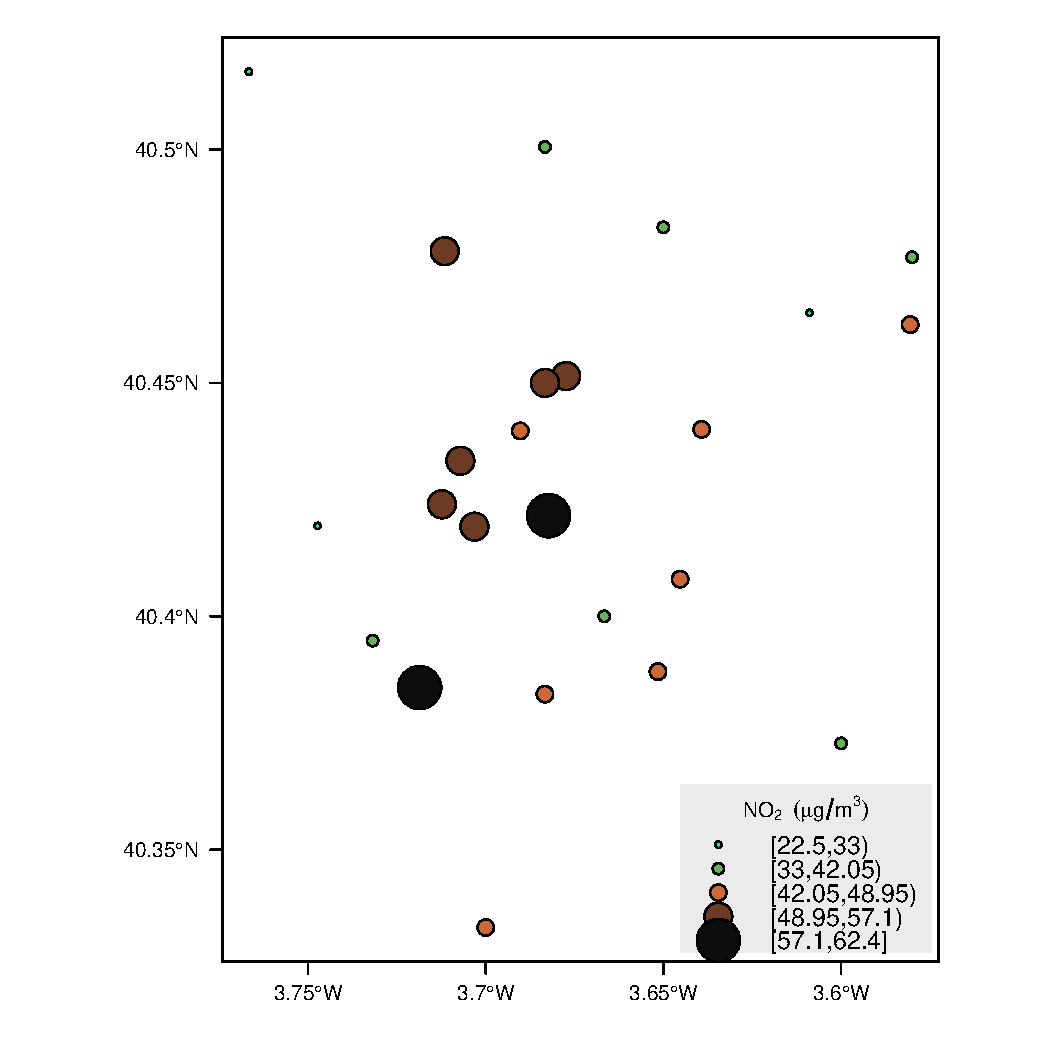
\includegraphics[width=.9\linewidth]{figs/airMadrid_classes.pdf}
\caption{\label{fig:org5254d1c}
Annual average of \(NO_2\) measurements in Madrid.}
\end{figure}

\subsection{Spatial Context with Underlying Layers and Labels}
\label{sec:org447233d}
The spatial distribution of the stations is better understood if
we add underlying layers with information about the spatial
context. 

\subsubsection{Static Image}
\label{sec:org87f66a8}
A suitable method is to download data from a provider such as Google
Maps\textsuperscript{\texttrademark} or OpenStreetMap and transform it adequately. There are several
packages that provide an interface to query several map servers. On
one hand, \texttt{RGoogleMaps}, \texttt{OpenStreetMaps}, and \texttt{ggmap} provide raster
images from static maps obtained from Google Maps, Stamen,
OpenStreetMap, etc.; on the other hand, \texttt{osmar} is able to access
OpenStreetMap data and convert it into classes provided by existing R
packages (mainly \texttt{sp} and \texttt{igraph0} objects).

Among these options, I have chosen the Stamen watercolor maps
available through the \texttt{ggmap} \cite{Kahle.Wickham2013} and
\texttt{OpenStreetMaps} packages \cite{Fellows.Stotz2013}. It is worth noting
that these map tiles are published by Stamen Design under a Creative
Commons licence CC BY-3.0 (Attribution). They produce these maps with
data by OpenStreetMap also published under a Creative Commons licence
BY-SA (Attribution - ShareAlike).

\begin{LaTeX}
\index\{Packages!ggmap@\texttt{ggmap}\}
\index\{Packages!OpenStreetMap@\texttt{OpenStreetMap}\}
\end{LaTeX}

\lstset{language=r,label= ,caption= ,captionpos=b,numbers=none}
\begin{lstlisting}
  madridBox <- bbox(NO2sp)

  ## ggmap solution
  library(ggmap)
  madridGG <- get_map(c(madridBox), maptype='watercolor', source='stamen')
\end{lstlisting}

\lstset{language=r,label= ,caption= ,captionpos=b,numbers=none}
\begin{lstlisting}
  ## OpenStreetMap solution
  library(OpenStreetMap)
  ul <- madridBox[c(4, 1)]
  lr <- madridBox[c(2, 3)]
  madridOM <- openmap(ul, lr, type='stamen-watercolor')
  madridOM <- openproj(madridOM)
\end{lstlisting}

\lstset{language=r,label= ,caption= ,captionpos=b,numbers=none}
\begin{lstlisting}
  NO2df <- data.frame(NO2sp)
  
  ## ggmap
  ggmap(madridGG) +
      geom_point(data=NO2df,
                 aes(long, lat, size=classNO2, fill=classNO2),
                 pch=21, col='black') +
         scale_fill_manual(values=airPal) +
         scale_size_manual(values=dentAQ*2)
  
  ##OpenStreetMap
  autoplot(madridOM) + 
      geom_point(data=NO2df,
                 aes(long, lat, size=classNO2, fill=classNO2),
                 pch=21, col='black') +
      scale_fill_manual(values=airPal) +
      scale_size_manual(values=dentAQ*2)  
  
\end{lstlisting}

Although \texttt{ggmap} is designed to work with the \texttt{ggplot2} package, the
result of \texttt{get\_map} is only a \texttt{raster} object with
attributes. Therefore, it can be easily displayed with \texttt{grid.raster}
as an underlying layer of the previous \texttt{spplot} result (Figure
\ref{fig:airMadrid_stamen}).

\lstset{language=r,label= ,caption= ,captionpos=b,numbers=none}
\begin{lstlisting}
  ## the 'bb' attribute stores the bounding box of the get_map result
  bbMap <- attr(madridGG, 'bb')
  ## This information is needed to resize the image with grid.raster
  height <- with(bbMap, ur.lat - ll.lat)
  width <- with(bbMap, ur.lon - ll.lon)
  
  pNO2 + layer(grid.raster(madridGG,
                            width=width, height=height,
                            default.units='native'),
               under=TRUE)
\end{lstlisting}

\begin{figure}[htbp]
\centering
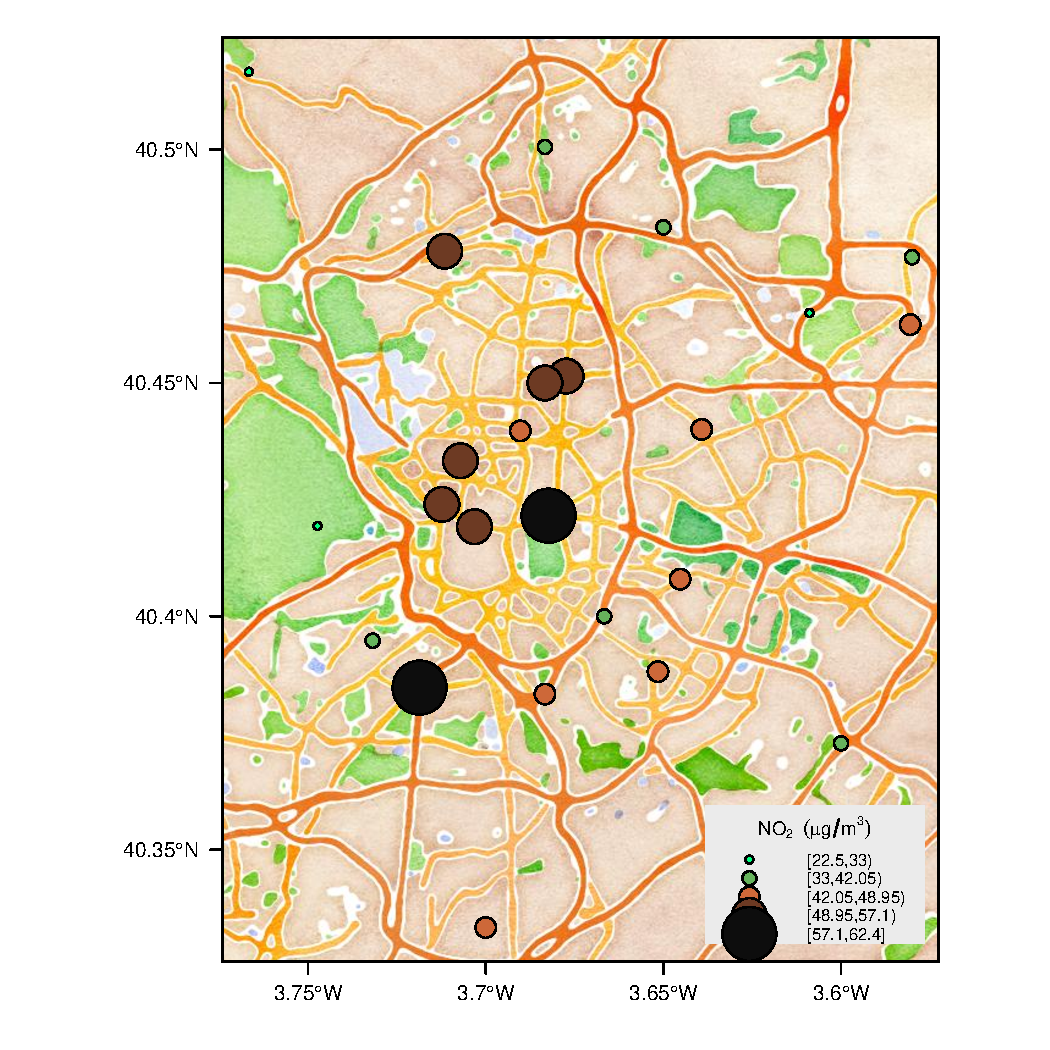
\includegraphics[width=.9\linewidth]{figs/airMadrid_stamen.pdf}
\caption{\label{fig:org261a66a}
Annual average of \(NO_2\) measurements in Madrid.}
\end{figure}

The result of \texttt{openmap} is more sophisticated but can also be
converted and displayed with \texttt{grid.raster}.
\lstset{language=r,label= ,caption= ,captionpos=b,numbers=none}
\begin{lstlisting}
  tile <- madridOM$tile[[1]]
  
  height <- with(tile$bbox, p1[2] - p2[2])
  width <- with(tile$bbox, p2[1] - p1[1])
  
  colors <- as.raster(matrix(tile$colorData,
                             ncol=tile$yres,
                             nrow=tile$xres,
                             byrow=TRUE))
  
  pNO2 + layer(grid.raster(colors,
                           width=width,
                           height=height,
                           default.units='native'),
               under=TRUE)
  
\end{lstlisting}

\subsubsection{Vector Data}
\label{sec:org44b86d4}
A major problem with the previous solution is that the user can
neither modify the image nor use its content to produce additional
information.  A different approach is to use digital vector data
(points, lines, and polygons). A popular format for vectorial data is
the shapefile, commonly used by public and private providers to
distribute information. A shapefile can be read with \texttt{readShapePoly}
and \texttt{readShapeLines} from the \texttt{rgdal} package. These functions produce
a \texttt{SpatialPolygonsDataFrame} and a \texttt{SpatialLinesDataFrame} objects,
respectively. These objects can be displayed with the \texttt{sp.polygons}
and \texttt{sp.lines} functions provided by the \texttt{sp} package.

For our example, the Madrid district and streets are available as
shapefiles from the nomecalles web service\footnote{\url{http://www.madrid.org/nomecalles/}}.

\begin{LaTeX}
\index{Data!nomecalles}
\index\{spTransform@\texttt{spTransform}\}
\index\{Packages!rgdal@\texttt{rgdal}\}
\index\{Packages!sp@\texttt{sp}\}
\index\{readShapeLines@\texttt{readShapeLines}\}
\index\{layer@\texttt{layer}\}
\index\{\sout{.trellis@\texttt\{}.trellis\}\}
\index\{sp.polygons@\texttt{sp.polygons}\}
\index\{sp.pointLabel@\texttt{sp.pointLabel}\}
\index\{sp.lines@\texttt{sp.lines}\}
\end{LaTeX}

\lstset{language=r,label= ,caption= ,captionpos=b,numbers=none}
\begin{lstlisting}
  library(maptools)
  library(rgdal)
    
  ## nomecalles http://www.madrid.org/nomecalles/Callejero_madrid.icm
  ## Form at http://www.madrid.org/nomecalles/DescargaBDTCorte.icm
  
  ## Madrid districts
  unzip('Distritos de Madrid.zip')
  distritosMadrid <- readShapePoly('Distritos de Madrid/200001331')
  proj4string(distritosMadrid) <- CRS("+proj=utm +zone=30")
  distritosMadrid <- spTransform(distritosMadrid, CRS=CRS("+proj=longlat +ellps=WGS84"))
  
  ## Madrid streets
  unzip('Callejero_ Ejes de viales.zip')
  streets <- readShapeLines('Callejero_ Ejes de viales/call2011.shp')
  streetsMadrid <- streets[streets$CMUN=='079',]
  proj4string(streetsMadrid) <- CRS("+proj=utm +zone=30")
  streetsMadrid <- spTransform(streetsMadrid, CRS=CRS("+proj=longlat +ellps=WGS84"))
\end{lstlisting}

These shapefiles can be included in the plot with the \texttt{sp.layout}
mechanism accepted by \texttt{spplot} or with the \texttt{layer} and \texttt{+.trellis}
functions from the \texttt{latticeExtra} package. The station codes are
placed with this same procedure using the \texttt{sp.pointLabel} function
from the \texttt{maptools} package. Figure \ref{fig:airMadrid} displays the
final result.

\begin{LaTeX}
\index\{Packages!maptools@\texttt{maptools}\}
\index\{sp.pointLabel@\texttt{sp.pointLabel}\}
\end{LaTeX}

\lstset{language=r,label= ,caption= ,captionpos=b,numbers=none}
\begin{lstlisting}
  spDistricts <- list('sp.polygons', distritosMadrid, fill='gray97', lwd=0.3)
  spStreets <- list('sp.lines', streetsMadrid, lwd=0.05)
  spNames <- list(sp.pointLabel, NO2sp,
                  labels=substring(NO2sp$codEst, 7),
                  cex=0.6, fontfamily='Palatino')
  
  spplot(NO2sp["classNO2"], col.regions=airPal, cex=dentAQ,
         edge.col='black', alpha=0.8,
         sp.layout=list(spDistricts, spStreets, spNames),
         scales=list(draw=TRUE),
         key.space=NO2key)
  
\end{lstlisting}

\lstset{language=r,label= ,caption= ,captionpos=b,numbers=none}
\begin{lstlisting}
  pNO2 +
      layer(sp.pointLabel(NO2sp,
                          labels=substring(NO2sp$codEst, 7),
                          cex=0.8, fontfamily='Palatino')
            ) +
      layer_({
          sp.polygons(distritosMadrid, fill='gray97', lwd=0.3)
          sp.lines(streetsMadrid, lwd=0.05)
      })
\end{lstlisting}

\begin{figure}[htbp]
\centering
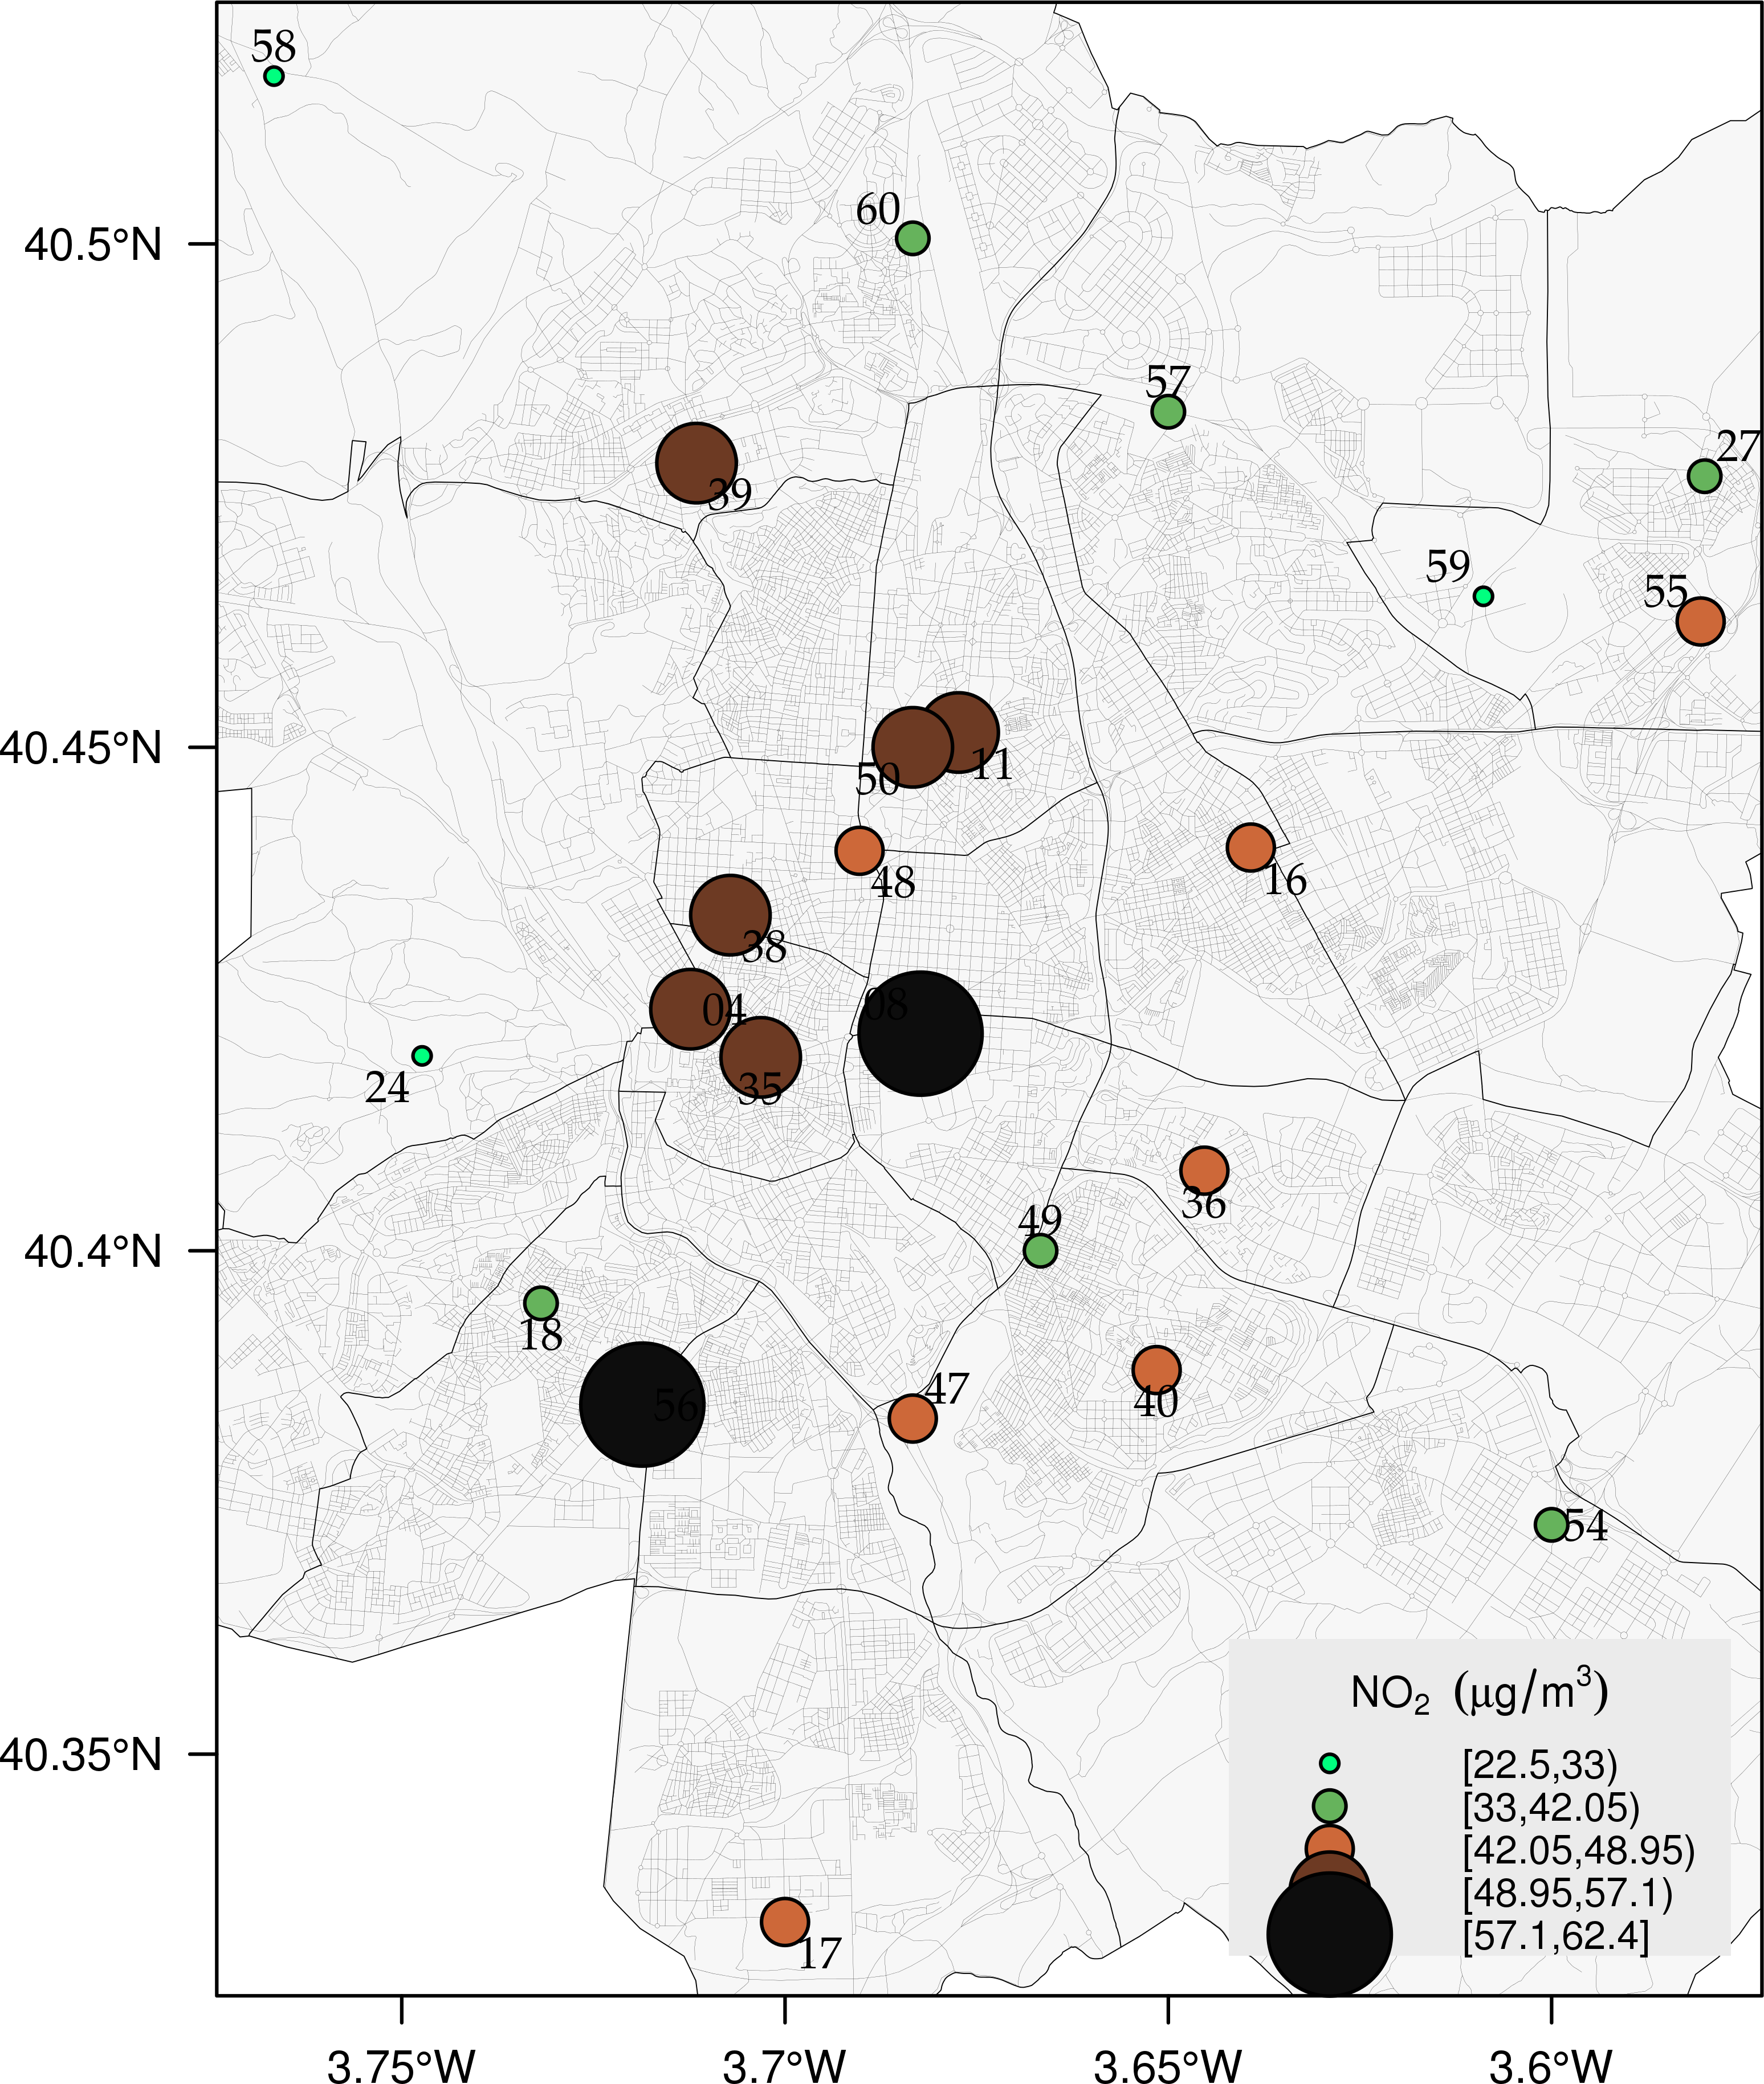
\includegraphics[width=.9\linewidth]{figs/airMadrid.png}
\caption{\label{fig:org304d847}
Annual average of \(NO_2\) measurements in Madrid using shapefiles (lines and polygons) and text as geographical context.}
\end{figure}

The \texttt{ggplot2} package is not able to work directly with
\texttt{SpatialLines*} or \texttt{SpatialPolygon*} objects. Instead, it includes
several \texttt{fortify} methods to convert objects from these classes into a
conventional \texttt{data.frame}. You should beware that the \texttt{fortify}
process for large objects (such as the \texttt{SpatialLinesDataFrame} in our
example) requires too much time to be completed.


\subsection{Spatial Interpolation}
\label{sec:org863e26d}
The measurements at discrete points give limited information about the
underlying process. It is quite common to approximate the spatial
distribution of the measured variable with the interpolation between
measurement locations. Selection of the optimal interpolation method
is outside the scope of this book. The following code illustrates an
easy solution using inverse distance weighted (IDW) interpolation with
the \texttt{gstat} package \cite{Pebesma2004} \emph{only} for illustration
purposes.

\begin{LaTeX}
\index\{Packages!gstat@\texttt{gstat}\}
\index\{Packages!krige@\texttt{krige}\}
\end{LaTeX}

\lstset{language=r,label= ,caption= ,captionpos=b,numbers=none}
\begin{lstlisting}
  library(gstat)
  
  airGrid <- spsample(NO2sp, type='regular', n=1e5)
  gridded(airGrid) <- TRUE
  airKrige <- krige(mean ~ 1, NO2sp, airGrid)
\end{lstlisting}

The result is a \texttt{SpatialPixelsDataFrame} that can be displayed with
\texttt{spplot} and combined with the previous layers and the measurement
station points (Figure \ref{fig:airMadrid_krige}).

\begin{LaTeX}
\index\{spplot@\texttt{spplot}\}
\index\{layer@\texttt{layer}\}
\index\{sp.polygons@\texttt{sp.polygons}\}
\index\{sp.lines@\texttt{sp.lines}\}
\index\{sp.points@\texttt{sp.points}\}
\end{LaTeX}

\lstset{language=r,label= ,caption= ,captionpos=b,numbers=none}
\begin{lstlisting}
spplot(airKrige["var1.pred"],
       col.regions=colorRampPalette(airPal)) +
  layer({
    sp.polygons(distritosMadrid, fill='transparent', lwd=0.3)
    sp.lines(streetsMadrid, lwd=0.07)
    sp.points(NO2sp, pch=21, alpha=0.8, fill='gray50', col='black')
    })
\end{lstlisting}

\begin{figure}[htbp]
\centering
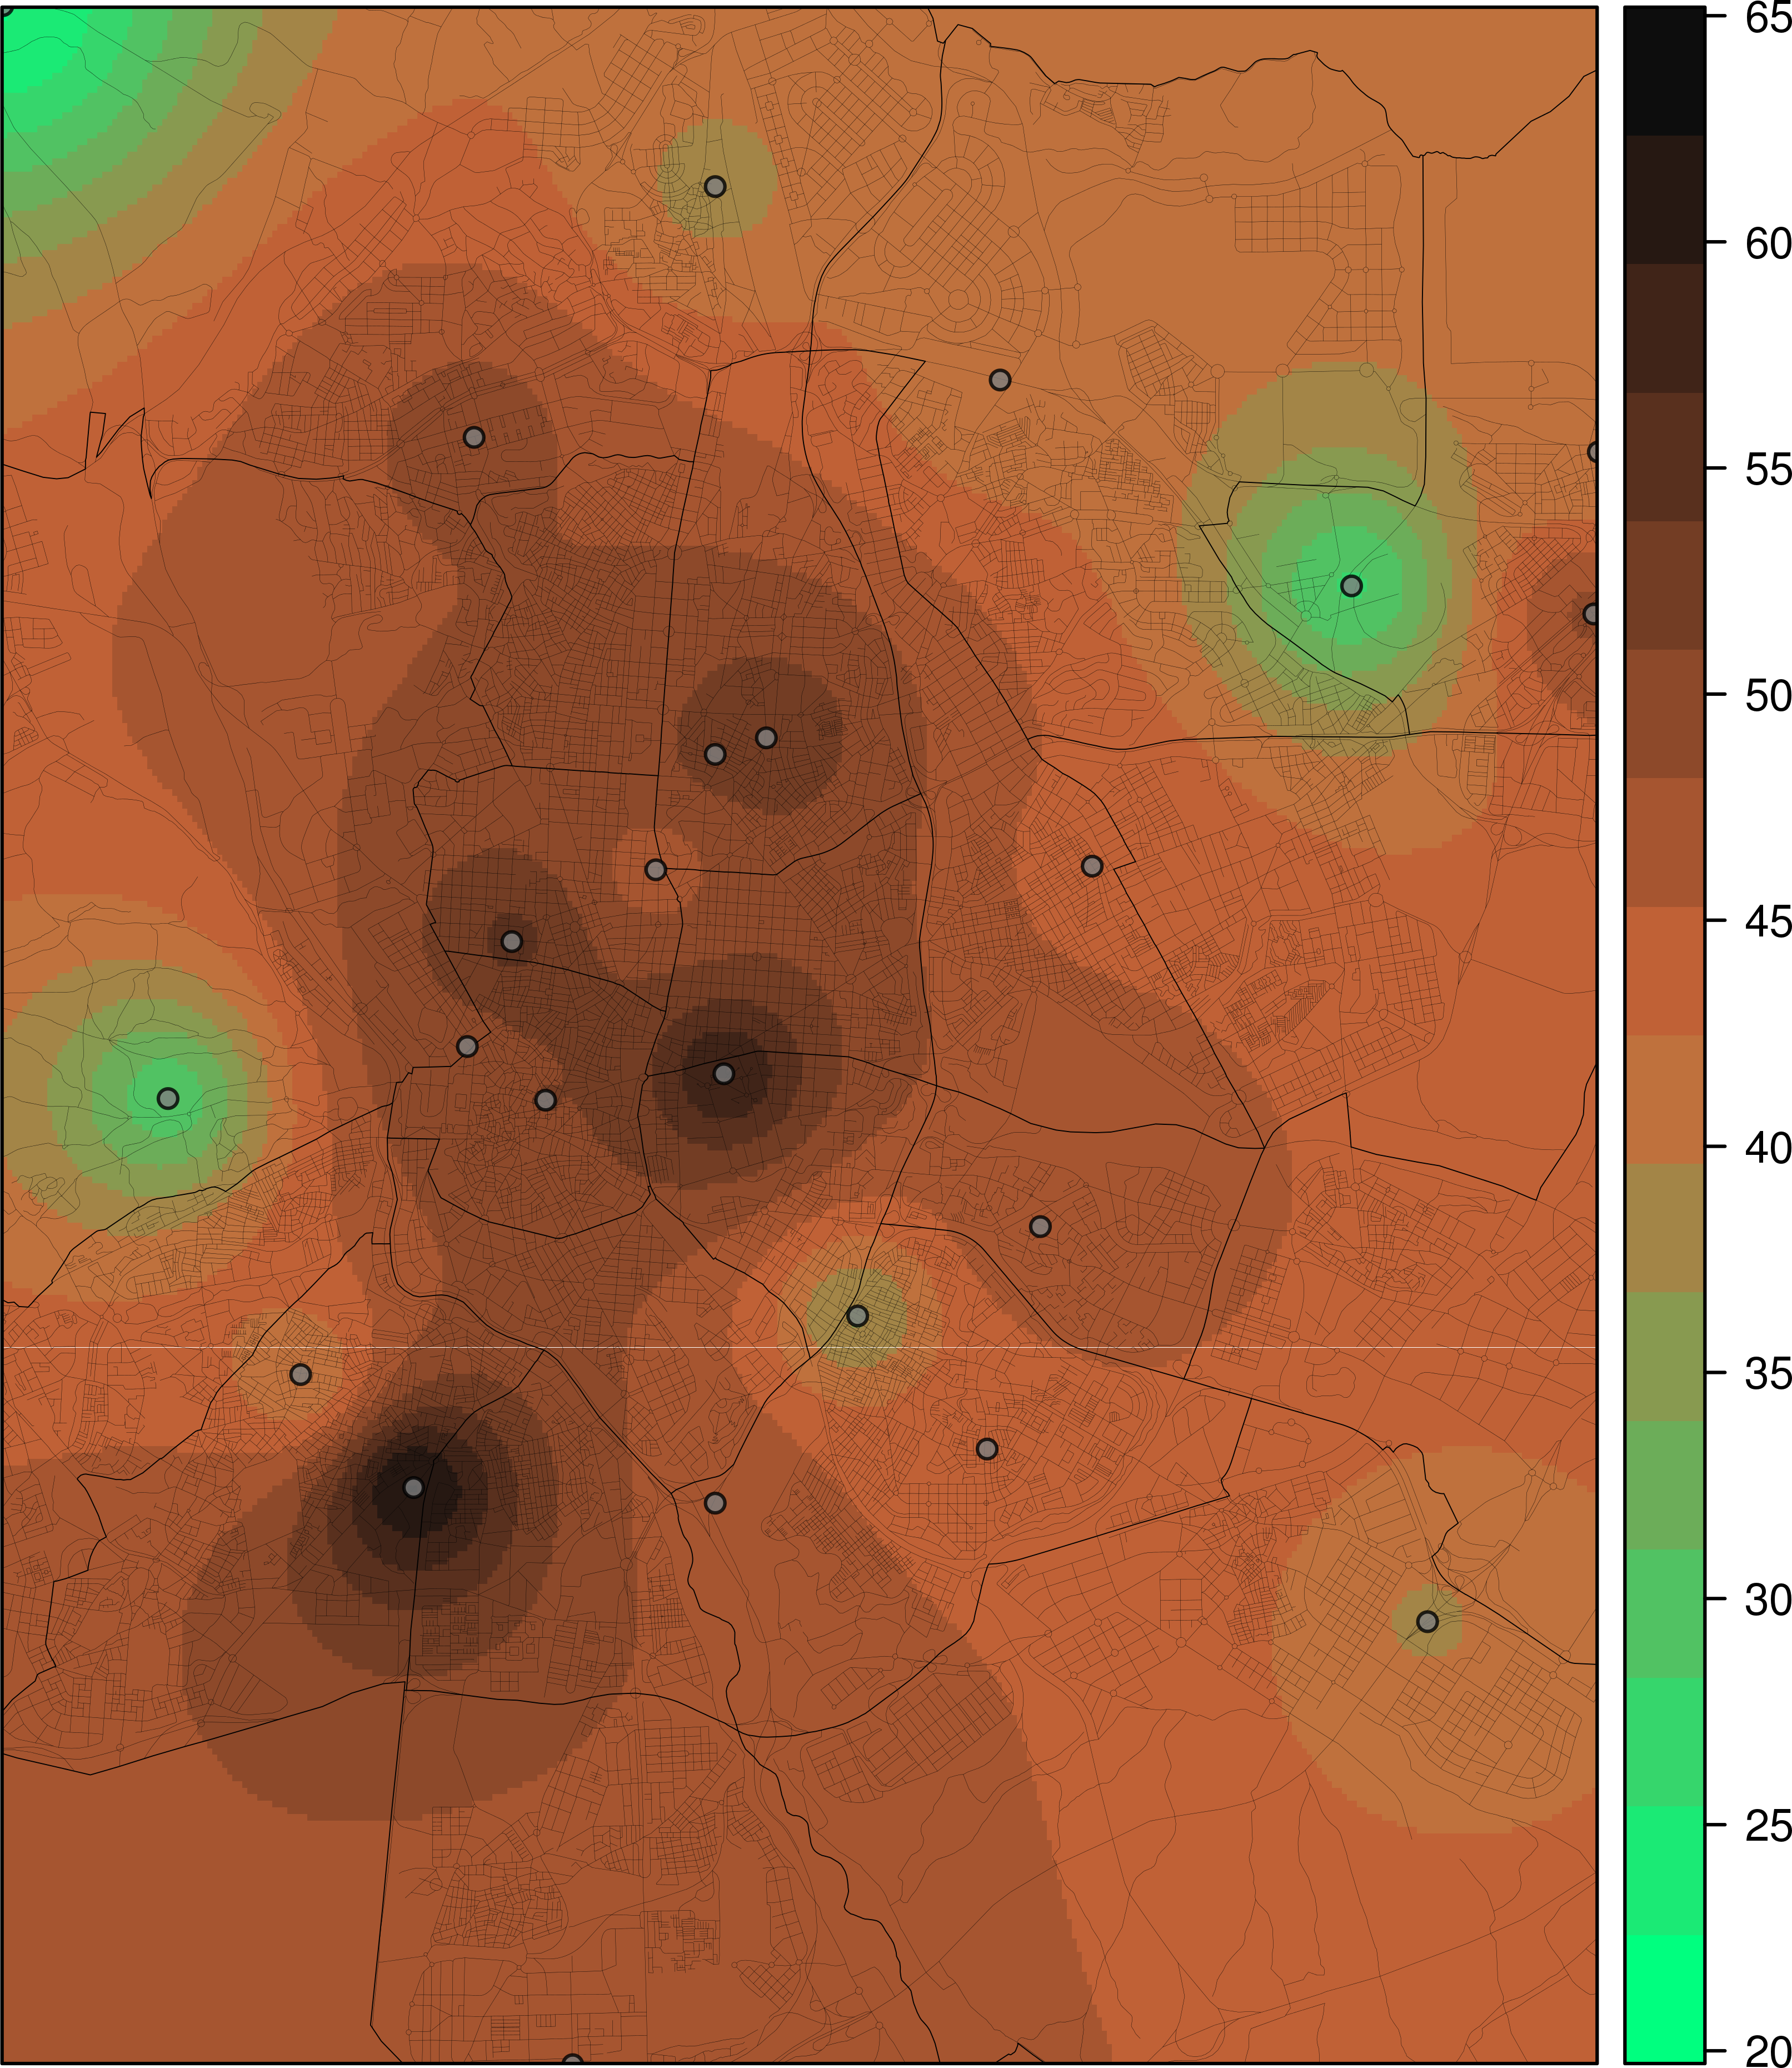
\includegraphics[width=.9\linewidth]{figs/airMadrid_krige.png}
\caption{\label{fig:orgd4e47f0}
Kriging annual average of \(NO_2\) measurements in Madrid.}
\end{figure}

\subsection{Export to Other Formats}
\label{sec:orgc97141f}

A different approach is to use an external data viewer, due to its
features or its large community of users. Two tools deserve to be
mentioned: GeoJSON rendered within GitHub repositories, and KML files
imported in Google Earth\texttrademark.

\subsubsection{GeoJSON and OpenStreetMap}
\label{sec:orgf5f3c1f}
GeoJSON is an open computer file format for encoding collections of
simple geographical features along with their nonspatial attributes
using JavaScript Object Notation (JSON). These files can be easily
rendered within GitHub repositories. GitHub uses Leaflet.js\footnote{\url{http://leafletjs.com/}} to
represent the data and MapBox\footnote{\url{http://www.mapbox.com/}} with OpenStreetMap\footnote{\url{http://www.openstreetmap.org/}} for the
underlying map data.

Our \texttt{SpatialPointsDataFrame} can be converted to a GeoJSON file with
\texttt{writeOGR} from the \texttt{rgdal} package. 

\begin{LaTeX}
\index\{Packages!rgdal@\texttt{rgdal}\}
\index\{writeOGR@\texttt{writeOGR}\}
\index{GeoJSON}
\end{LaTeX}

\lstset{language=r,label= ,caption= ,captionpos=b,numbers=none}
\begin{lstlisting}
library(rgdal)
writeOGR(NO2sp, 'data/NO2.geojson', 'NO2sp', driver='GeoJSON')
\end{lstlisting}

Figure \ref{fig:geojson} shows a snapshot of the rendering of this
GeoJSON file, available from the GitHub repository. There you can zoom
on the map and click on the stations to display the data.

\begin{LaTeX}
\begin{figure}
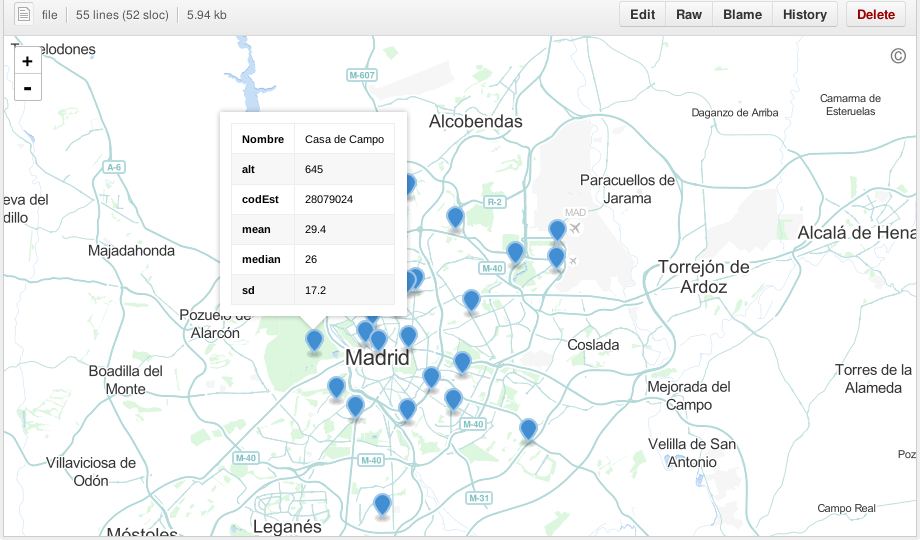
\includegraphics[width=0.9\textwidth]{figs/geojson.png}
\caption{\label{fig:geojson}$NO_2$ data in a GeoJSON file rendered within the GitHub repository.}
\end{figure}
\end{LaTeX}

\subsubsection{Keyhole Markup Language}
\label{sec:orgc29ddd7}

Keyhole Markup Language (KML) is a file format to display geographic
data within Internet-based, two-dimensional maps and three-dimensional
Earth browsers. KML uses a tag-based structure with nested elements
and attributes, and is based on the XML standard. KML became an
international standard of the Open Geospatial Consortium
in 2008. Google Earth was the first program able to view and
graphically edit KML files, although Marble, an open-source project,
also offers KML support.

\begin{LaTeX}
\index\{Packages!rgdal@\texttt{rgdal}\}
\index\{Packages!plotKML@\texttt{plotKML}\}
\index{KML}
\end{LaTeX}

There are several packages able to generate KML files. For example,
the \texttt{writeOGR} function from the \texttt{rgdal} package can also write KML
files:
\lstset{language=r,label= ,caption= ,captionpos=b,numbers=none}
\begin{lstlisting}
  library(rgdal)
  writeOGR(NO2sp, dsn='NO2_mean.kml', layer='mean', driver='KML')
\end{lstlisting}

However, the \texttt{plotKML} package provides a simpler interface and
includes a wide set of options:
\lstset{language=r,label= ,caption= ,captionpos=b,numbers=none}
\begin{lstlisting}
  library(plotKML)
  plotKML(NO2sp["mean"], points_names=NO2sp$codEst)
\end{lstlisting}

Both functions produce a file that can be directly opened with Google
Earth or Marble.

\subsection{Interactive}
\label{sec:org344ccb1}
Additional Information with Tooltips and Hyperlinks
\subsubsection{mapview}
\label{sec:orgc0d1838}
\lstset{language=r,label= ,caption= ,captionpos=b,numbers=none}
\begin{lstlisting}
mapview(NO2sp, zcol = "mean", cex = "mean")
\end{lstlisting}

\subsection{\floweroneleft gridSVG}
\label{sec:org669e15d}
Now, let's suppose you need to know the median and standard deviation
of the time series of a certain station. Moreover, you would like to
watch the photography of that station; or even better, you wish to visit
its webpage for additional information. A frequent solution is to
produce interactive graphics with tooltips and hyperlinks.

The \texttt{gridSVG} package is able to create an SVG graphic, where each
component owns a \texttt{title} attribute; the content of this attribute is
commonly displayed as a tooltip when the mouse hovers over the
element. The content of this attribute can be modified thanks to the
\texttt{grid.garnish} function. Moreover, the \texttt{grid.hyperlink} function can
add hyperlinks to the correspondent graphical element.

The tooltips will display the photography of the station, the name of
the station, and the statistics previously calculated with \texttt{aggregate}
in the first step of this chapter.  The station images are downloaded
from the Munimadrid webpage. The \texttt{htmlParse} function from the \texttt{XML}
package parses each station page, and the station photograph is
extracted with \texttt{getNodeSet} and \texttt{xmlAttrs}.

\begin{LaTeX}
\index\{Packages!XML@\texttt{XML}\}
\index\{htmlParse@\texttt{htmlParse}\}
\index\{getNodeSet@\texttt{getNodeSet}\}
\end{LaTeX}

\lstset{language=r,label= ,caption= ,captionpos=b,numbers=none}
\begin{lstlisting}
  library(XML)

  old <- setwd('images')
  for (i in 1:nrow(NO2df)){
    codEst <- NO2df[i, "codEst"]
    ## Webpage of each station
    codURL <- as.numeric(substr(codEst, 7, 8))
    rootURL <- 'http://www.mambiente.munimadrid.es'
    stationURL <- paste(rootURL,
                        '/opencms/opencms/calaire/contenidos/estaciones/estacion',
                        codURL, '.html', sep='')
    content <- htmlParse(stationURL, encoding='utf8')
    ## Extracted with http://www.selectorgadget.com/
    xPath <- '//*[contains(concat( " ", @class, " " ), concat( " ", "imagen_1", " " ))]'
    imageStation <- getNodeSet(content, xPath)[[1]]
    imageURL <- xmlAttrs(imageStation)[1]
    imageURL <- paste(rootURL, imageURL, sep='')
    download.file(imageURL, destfile=paste(codEst, '.jpg', sep=''))
  }
  setwd(old)
\end{lstlisting}

Next, we attach the hyperlink and the SVG information to each
circle.


\begin{LaTeX}
\index\{Packages!gridSVG@\texttt{gridSVG}\}
\index{JavaScript}
\index\{grid.garnish@\texttt{grid.garnish}\}
\index\{grid.hyperlink@\texttt{grid.hyperlink}\}
\index\{grid.export@\texttt{grid.export}\}
\end{LaTeX}

\lstset{language=r,label= ,caption= ,captionpos=b,numbers=none}
\begin{lstlisting}
  print(pNO2 + layer_(sp.polygons(distritosMadrid, fill='gray97', lwd=0.3)))
\end{lstlisting}

\lstset{language=r,label= ,caption= ,captionpos=b,numbers=none}
\begin{lstlisting}
  library(gridSVG)
  
  NO2df <- as.data.frame(NO2sp)
  
  tooltips <- sapply(seq_len(nrow(NO2df)), function(i){
    codEst <- NO2df[i, "codEst"]
    ## Information to be attached to each line
    stats <- paste(c('Mean', 'Median', 'SD'),
                   signif(NO2df[i, c('mean', 'median', 'sd')], 4),
                   sep=' = ', collapse='<br />')
    ## Station photograph 
    imageURL <- paste('images/', codEst, '.jpg', sep='')
    imageInfo <- paste("<img src=", imageURL,
                       " width='100' height='100' />", sep='')
    ## Text to be included in the tooltip
    nameStation <- paste('<b>', 
                         as.character(NO2df[i, "Nombre"]),
                         '</b>', sep='')
    info <- paste(nameStation, stats, sep='<br />')
    ## Tooltip includes the image and the text
    paste(imageInfo, info, sep='<br />')
  })
  grid.garnish('points.panel', title=tooltips,  grep=TRUE, group=FALSE)
\end{lstlisting}


\lstset{language=r,label= ,caption= ,captionpos=b,numbers=none}
\begin{lstlisting}
  ## Webpage of each station
  rootURL <- 'http://www.mambiente.munimadrid.es'
  urlList <- sapply(seq_len(nrow(NO2df)), function(i){
    codEst <- NO2df[i, "codEst"]
    codURL <- as.numeric(substr(codEst, 7, 8))
    stationURL <- paste(rootURL,
                        '/opencms/opencms/calaire/contenidos/estaciones/estacion',
                        codURL, '.html', sep='')
    })
  
  grid.hyperlink('points.panel', urlList, grep=TRUE, group=FALSE)
\end{lstlisting}

The \texttt{title} attribute can be accessed with the JavaScript plug-ins
jQuery\footnote{\url{http://jquery.com/}} and jQuery UI\footnote{\url{http://jqueryui.com/}} to display tooltips when the mouse
hovers over each station. The \texttt{grid.script} function creates objects
containing links to these plug-ins. And \texttt{grid.export} uses these
objects to produce an SVG document with script elements.

\begin{LaTeX}
\index{jQuery} 
\index{jQuery UI}
\end{LaTeX}

\lstset{language=r,label= ,caption= ,captionpos=b,numbers=none}
\begin{lstlisting}
  ## Add jQuery and jQuery UI scripts
  grid.script(file='http://code.jquery.com/jquery-1.8.3.js')
  grid.script(file='http://code.jquery.com/ui/1.9.2/jquery-ui.js')
  ## Simple JavaScript code to initialize the tooltip
  grid.script(file='js/myTooltip.js')
  ## Produce the SVG graphic: the results of grid.garnish,
  ## grid.hyperlink and grid.script are converted to SVG code
  grid.export('figs/airMadrid.svg')
\end{lstlisting}

These plug-ins will work only after the file \texttt{airMadrid.svg} created by
\texttt{grid.export} is inserted in a HTML file with standard headers. Figure
\ref{fig:airMadridTooltip} shows a capture of the result.

\lstset{language=r,label= ,caption= ,captionpos=b,numbers=none}
\begin{lstlisting}
  htmlBegin <- '<!DOCTYPE html>
  <html>
  <head>
  <title>Tooltips with jQuery and gridSVG</title>
  <link rel="stylesheet" type="text/css" href="http://code.jquery.com/ui/1.9.2/themes/smoothness/jquery-ui.css" />
  <meta charset="utf-8">
  </head>
  <body>'
  
  htmlEnd <- '</body> </html>'
    
  svgText <- paste(readLines('figs/airMadrid.svg'), collapse='\n')
    
  writeLines(paste(htmlBegin, svgText, htmlEnd, sep='\n'),
             'airMadrid.html')
\end{lstlisting}


\begin{LaTeX}
\begin{figure}
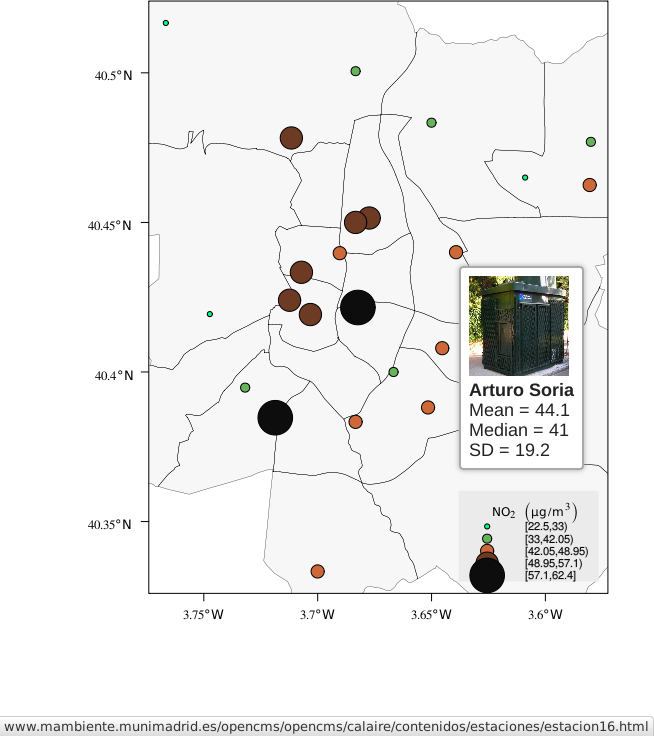
\includegraphics[width=0.9\textwidth]{figs/airMadridTooltip.png}
\caption{\label{fig:airMadridTooltip}Tooltips generated with \texttt{gridSVG} using jQuery and jQuery UI.}
\end{figure}
\end{LaTeX}


\section{Choropleth Maps}
\label{sec-1}
\label{sec:multiChoropleth}
A choropleth map shades regions according to the measurement of a
variable displayed on the map. The choropleth map is an appropiate
tool to visualize a variable uniformly distributed within each
region, changing only at the region boundaries. This method
performs correctly with homogeneous regions, both in size and
shape.  

This section details how to create a multivariate choropleth map to
show the results of the 2011 Spanish general elections. It is inspired
by the infographic from the \emph{New York Times\footnote{\url{http://www.nytimes.com/interactive/2009/03/10/us/20090310-immigration-explorer.html}}}, a multivariate
choropleth map of the inmigration behavior in the United States.

\lstset{language=R,numbers=none}
\begin{lstlisting}
votes2011 <- read.csv('data/votes2011.csv',
		      colClasses=c('factor', 'factor', 'numeric', 'numeric'))
\end{lstlisting}

The next section describes how to define a \texttt{SpatialPolygonsDataFrame}
with the data from this \texttt{data.frame} and the spatial information of
the administrative boundaries from a shapefile. You can skip it for
later reading if you are not interested in this procedure and jump to
the section \ref{sec:map} where the maps are produced.

\subsection{\floweroneleft Administrative Boundaries}
\label{sec-1-1}

The Spanish administrative boundaries are available as shapefiles at
the INE (Instituto Nacional de Estadística) webpage\footnote{\url{http://www.ine.es/} > Products and services > Publications > Download the PC-Axis program > Municipal maps}. Both the
municipalities, \texttt{espMap}, and province boundaries, \texttt{provinces}, are
read as \texttt{SpatialPolygonsDataFrame} with \texttt{readShapePoly}.

\index{Packages!maps@\texttt{maps}}
\index{Packages!maptools@\texttt{maptools}}
\index{Packages!rgeos@\texttt{rgeos}}
\index{Packages!sp@\texttt{sp}}
\index{Packages!latticeExtra@\texttt{latticeExtra}}

\lstset{language=R,numbers=none}
\begin{lstlisting}
library(sp)
library(maptools)
\end{lstlisting}

\index{INE}
\index{readShapePoly@\texttt{readShapePoly}}
\index{Encoding@\texttt{Encoding}}

\lstset{language=R,numbers=none}
\begin{lstlisting}
old <- setwd(tempdir())
download.file('http://goo.gl/TIvr4', 'mapas_completo_municipal.rar')
system2('unrar', c('e', 'mapas_completo_municipal.rar'))
espMap <- readShapePoly(fn="esp_muni_0109")
Encoding(levels(espMap$NOMBRE)) <- "latin1"

provinces <- readShapePoly(fn="spain_provinces_ag_2")
setwd(old)
\end{lstlisting}

Some of the polygons are repeated and can be dissolved with
\texttt{unionSpatialPolygons} (the \texttt{rgeos} package must be installed).
\index{unionSpatialPolygons@\texttt{unionSpatialPolygons}}
\lstset{language=R,numbers=none}
\begin{lstlisting}
## dissolve repeated polygons
espPols <- unionSpatialPolygons(espMap, espMap$PROVMUN)
\end{lstlisting}

Spanish maps are commonly displayed with the Canarian islands next
to the peninsula. First we have to extract the polygons of the
islands and the polygons of the peninsula, and then shift the
coordinates of the islands with \texttt{elide}. Finally, a new
\texttt{SpatialPolygons} object binds the shifted islands with the
peninsula.

\lstset{language=R,numbers=none}
\begin{lstlisting}
## Extract Canarias islands from the SpatialPolygons object
canarias <-  sapply(espPols@polygons, function(x)substr(x@ID, 1, 2) %in% c("35",  "38"))
peninsulaPols <- espPols[!canarias]
islandPols <- espPols[canarias]

## Shift the island extent box to position them at the bottom right corner
dy <- bbox(peninsulaPols)[2,1] - bbox(islandPols)[2,1]
dx <- bbox(peninsulaPols)[1,2] - bbox(islandPols)[1,2]
islandPols2 <- elide(islandPols, shift=c(dx, dy))
bbIslands <- bbox(islandPols2)

## Bind Peninsula (without islands) with shifted islands
espPols <- rbind(peninsulaPols, islandPols2)
\end{lstlisting}

The final step is to link the data with the polygons. The \texttt{ID} slot of
each polygon is the key to find the correspondent registry in the
\texttt{votes2011} dataset.
\lstset{language=R,numbers=none}
\begin{lstlisting}
## Match polygons and data using ID slot and PROVMUN column
IDs <- sapply(espPols@polygons, function(x)x@ID)
idx <- match(IDs, votes2011$PROVMUN)

##Places without information
idxNA <- which(is.na(idx))

##Information to be added to the SpatialPolygons object
dat2add <- votes2011[idx, ]

## SpatialPolygonsDataFrame uses row names to match polygons with data
row.names(dat2add) <- IDs
espMapVotes <- SpatialPolygonsDataFrame(espPols, dat2add)

## Drop those places without information
espMapVotes <- espMapVotes[-idxNA, ]
\end{lstlisting}
\subsection{Map}
\label{sec-1-2}
\label{sec:map}
The \texttt{SpatialPolygonsDataFrame} constructed in the previous section
contains two main variables: \texttt{whichMax}, the name of the predominant
political option, and \texttt{pcMax}, the percentage of votes obtained by
this political option.

\texttt{whichMax} is a categorical value with four levels: the two main
parties (\texttt{PP} and \texttt{PSOE}), the abstention results (\texttt{ABS}), and the
rest of the parties (\texttt{OTH}). Figure \ref{fig:whichMax} encodes these levels
with a qualitative palette with constant hues and varying chroma and
luminance for each class using the package \texttt{colorspace}
\cite{Zeileis.Hornik.ea2009}. In order to improve the color
discrimination, hues are equally spaced along the HCL (Hue, Chroma,
Luminance) based color wheel.

\index{Packages!colorspace@\texttt{colorspace}}
\index{rainbow_hcl@\texttt{rainbow\_hcl}}
\lstset{language=R,numbers=none}
\begin{lstlisting}
library(colorspace)  

classes <- levels(factor(espMapVotes$whichMax))
nClasses <- length(classes)

qualPal <- rainbow_hcl(nClasses, start=30, end=300)
\end{lstlisting}

For the definition of a combined palette in the next section, it is
interesting to note that the colors provided by \texttt{rainbow\_hcl} can be
obtained with the following code where the distances between hues and
their values are computed explicitly.
\index{hcl@\texttt{hcl}}
\lstset{language=R,numbers=none}
\begin{lstlisting}
## distance between hues
step <- 360/nClasses 
## hues equally spaced
hue = (30 + step*(seq_len(nClasses)-1))%%360 
qualPal <- hcl(hue, c=50, l=70)
\end{lstlisting}

\lstset{language=R,numbers=none}
\begin{lstlisting}
spplot(espMapVotes["whichMax"], col='transparent', col.regions=qualPal)
\end{lstlisting}

\begin{figure}[htb]
\centering
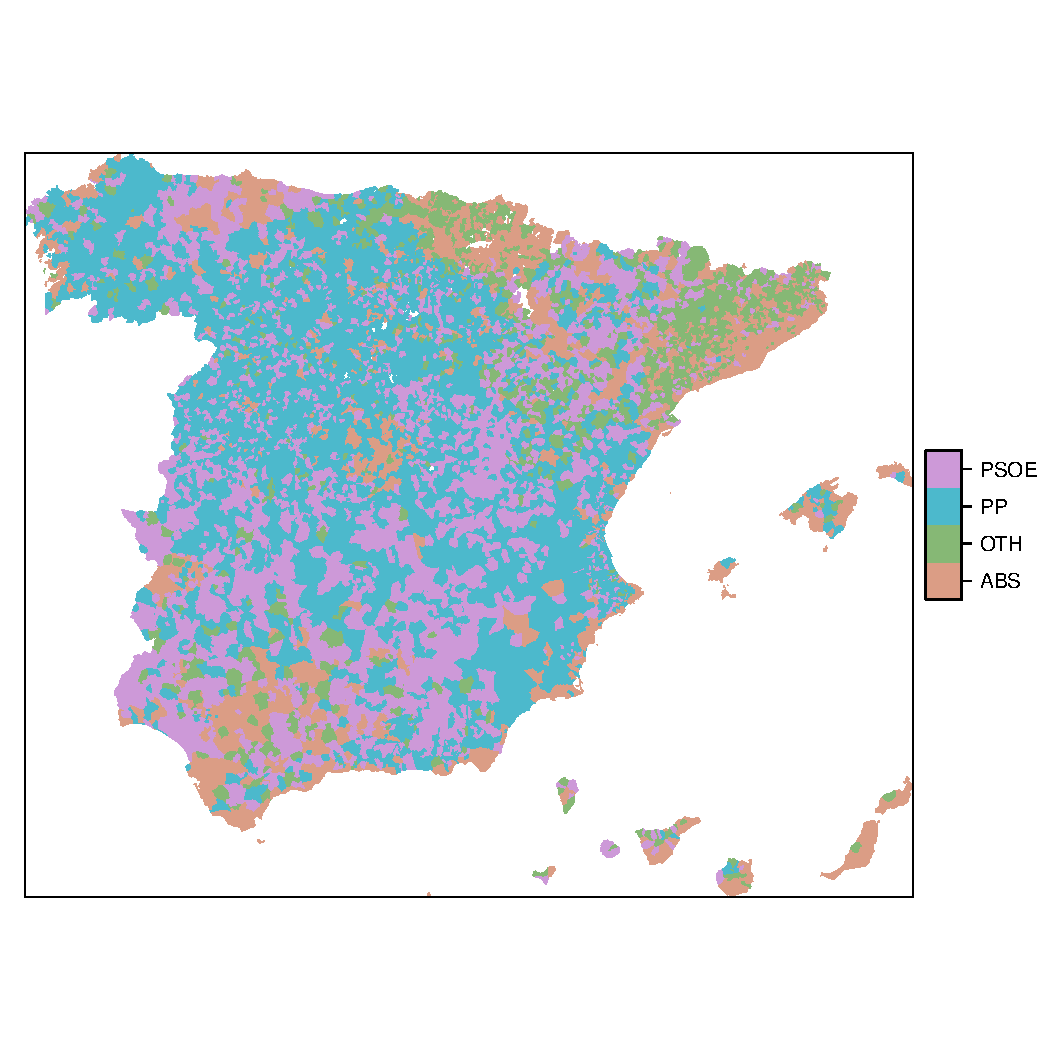
\includegraphics[width=.9\linewidth]{figs/whichMax.pdf}
\caption{\label{fig:whichMax}Categorical choropleth map displaying the name of the predominant political option in each municipality in the 2011 Spanish general elections.}
\end{figure}

On the other hand, \texttt{pcMax} is a quantitative variable that can be
adequately displayed with a sequential palette (Figure \ref{fig:pcMax}).
\lstset{language=R,numbers=none}
\begin{lstlisting}
quantPal <- rev(heat_hcl(16))
spplot(espMapVotes["pcMax"], col='transparent', col.regions=quantPal)
\end{lstlisting}

\begin{figure}[htb]
\centering
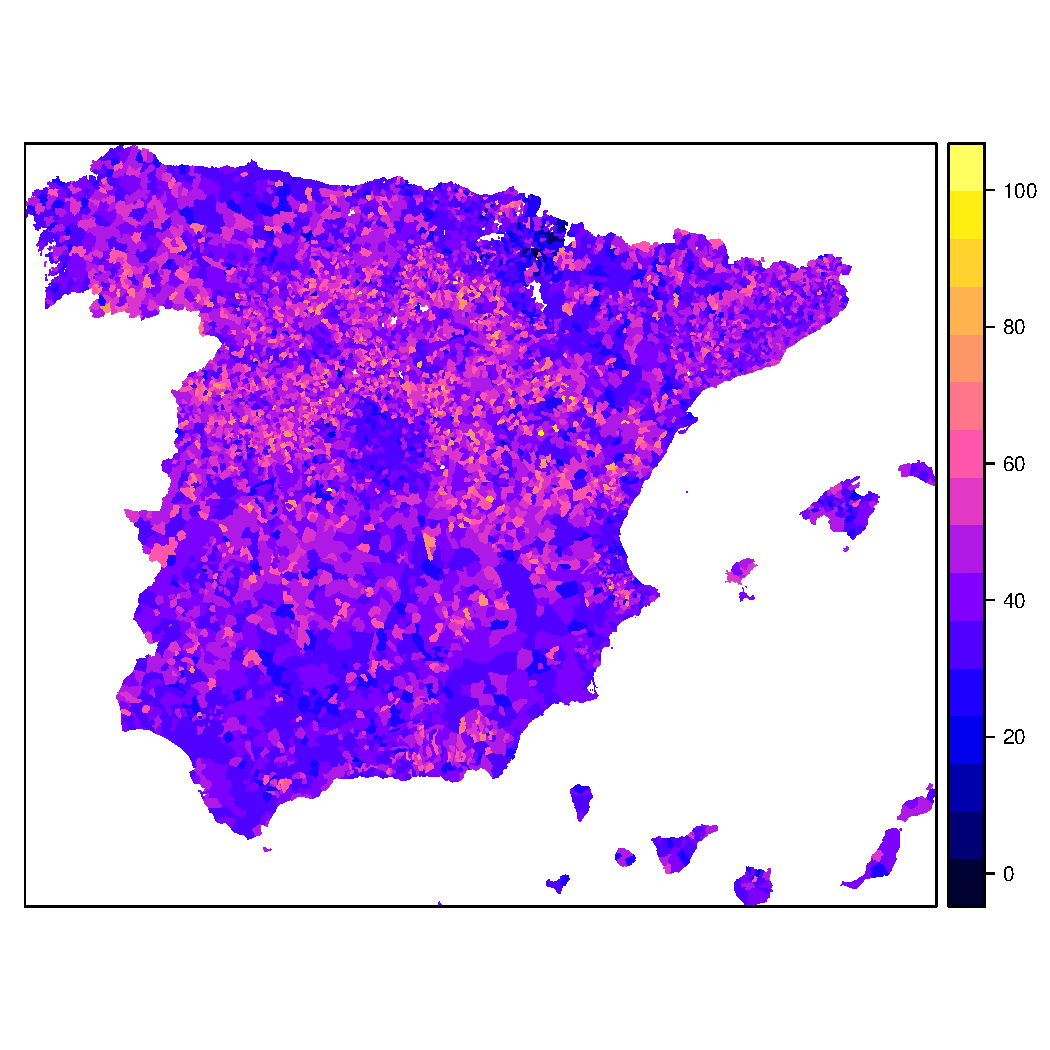
\includegraphics[width=.9\linewidth]{figs/pcMax.pdf}
\caption{\label{fig:pcMax}Quantitative choropleth map displaying the percentage of votes obtained by the predominant political option in each municipality in the 2011 Spanish general elections.}
\end{figure}
\subsection{\floweroneleft Categorical and Quantitative Variables Combined in a Multivariate Choropleth Map}
\label{sec-1-3}
Following the inspiring example of the infographic from the \emph{New
York Times}, we will combine both choropleth maps to produce a
multivariate map: the hue of each polygon will be determined by
the name of the predominant option (\texttt{whichMax}) but the chroma and
luminance will vary according to the percentage of votes
(\texttt{pcMax}). Hues are computed with the same method as in Figure
\ref{fig:whichMax}, while the corresponding values of chroma and
luminance are calculated with the \texttt{sequential\_hcl} function.

\index{sequential_hcl@\texttt{sequential\_hcl}}
\lstset{language=R,numbers=none}
\begin{lstlisting}
classes <- levels(factor(espMapVotes$whichMax))
nClasses <- length(classes)
step <- 360/nClasses
multiPal <- lapply(1:nClasses, function(i){
    rev(sequential_hcl(16, h = (30 + step*(i-1))%%360))
    })
\end{lstlisting}

With this multivariate palette we can produce a list of maps
extracting the polygons according to each class and filling with
the appropiate color from this palette. The resulting list of
\texttt{trellis} objects can be combined with \texttt{Reduce} and the
\texttt{+.trellis} function of the \texttt{latticeExtra} and produce a \texttt{trellis}
object.

It is important to note that, to ensure the legend's homogeneity, the
breakpoints defined by the \texttt{at} argument are the same for all the
individual maps.

\index{Reduce@\texttt{Reduce}} \index{spplot@\texttt{spplot}}
\lstset{language=R,numbers=none}
\begin{lstlisting}
pList <- lapply(1:nClasses, function(i){
    ## Only those polygons corresponding to a level are selected
    mapClass <- espMapVotes[espMapVotes$whichMax==classes[i],]
    pClass <- spplot(mapClass['pcMax'], col.regions=multiPal[[i]],
		     col='transparent',
		     ## labels only needed in the last legend
		     colorkey=(if (i==nClasses) TRUE else list(labels=rep('', 6))),
		     at = seq(0, 100, by=20))
})

p <- Reduce('+', pList)
\end{lstlisting}

The legend of this \texttt{trellis} object must be defined
manually. The main operation is to merge the legends from the
components of the list of maps to obtain a bivariate
legend. 

The first step is to add a title to each individual legend.  This is a
little complex because \texttt{levelplot} (the engine under the \texttt{spplot}
method) does not include a title in its color key. The solution is to
define a function to add the title and include it as an argument to
the legend component of each \texttt{trellis} object. The \texttt{print.trellis}
method will process this function when displaying the \texttt{trellis}
object. The \texttt{frameGrob} and \texttt{packGrob} of the \texttt{grid} package will do
the main work inside this function.

\index{textGrob@\texttt{textGrob}}
\index{packGrob@\texttt{packGrob}}
\index{Packages!grid@\texttt{grid}}
\lstset{language=R,numbers=none}
\begin{lstlisting}
## Function to add a title to a legend
addTitle <- function(legend, title){
  titleGrob <- textGrob(title, gp=gpar(fontsize=8), hjust=1, vjust=1)
  ## retrieve the legend from the trellis object
  legendGrob <- eval(as.call(c(as.symbol(legend$fun), legend$args)))
  ## Layout of the legend WITH the title
  ly <- grid.layout(ncol=1, nrow=2,
		    widths=unit(0.9, 'grobwidth', data=legendGrob))
  ## Create a frame to host the original legend and the title
  fg <- frameGrob(ly, name=paste('legendTitle', title, sep='_'))
  ## Add the grobs to the frame
  pg <- packGrob(fg, titleGrob, row=2)
  pg <- packGrob(pg, legendGrob, row=1)
  }

## Access each trellis object from pList...
for (i in seq_along(classes)){
  ## extract the legend (automatically created by spplot)...
  lg <- pList[[i]]$legend$right
  ## ... and add the addTitle function to the legend component of each trellis object
  pList[[i]]$legend$right <- list(fun='addTitle',
				  args=list(legend=lg, title=classes[i]))
}
\end{lstlisting}

Now that every component of \texttt{pList} includes a legend with a title,
the legend of the \texttt{p} trellis object can be modified to store the
merged legends from the set of components of \texttt{pList}.

\lstset{language=R,numbers=none}
\begin{lstlisting}
## List of legends
legendList <- lapply(pList, function(x){
  lg <- x$legend$right
  clKey <- eval(as.call(c(as.symbol(lg$fun), lg$args)))
  clKey
})

## Function to pack the list of legends in a unique legend
## Adapted from latticeExtra::: mergedTrellisLegendGrob
packLegend <- function(legendList){
  N <- length(legendList)
  ly <- grid.layout(nrow = 1,  ncol = N)
  g <- frameGrob(layout = ly, name = "mergedLegend")
  for (i in 1:N) g <- packGrob(g, legendList[[i]], col = i)
  g
}

## The legend of p will include all the legends
p$legend$right <- list(fun = 'packLegend',  args = list(legendList = legendList))
\end{lstlisting}

Figure \ref{fig:mapLegends} displays the result with the province boundaries
superposed (only for the peninsula due to a problem with the
definition of boundaries the Canarian islands in the file) and a
rectangle to separate the Canarian islands from the remainder of the
map.

\lstset{language=R,numbers=none}
\begin{lstlisting}
canarias <- provinces$PROV %in% c(35, 38)
peninsulaLines <- provinces[!canarias,]

p +
  layer(sp.polygons(peninsulaLines,  lwd = 0.1)) +
  layer(grid.rect(x=bbIslands[1,1], y=bbIslands[2,1],
		  width=diff(bbIslands[1,]),
		  height=diff(bbIslands[2,]),
		  default.units='native', just=c('left', 'bottom'),
		  gp=gpar(lwd=0.5, fill='transparent')))
\end{lstlisting}

\begin{figure}[htb]
\centering
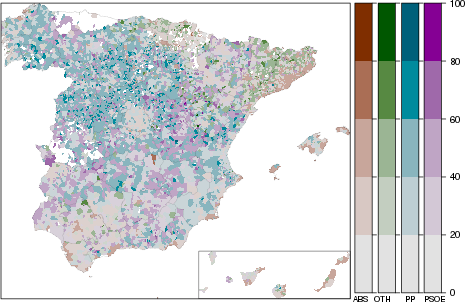
\includegraphics[width=.9\linewidth]{figs/mapLegends.png}
\caption{\label{fig:mapLegends}Spanish general elections results. The map shows the result of the most voted option in each municipality.}
\end{figure}


\section{Raster Maps}
\label{sec-1}
\label{cha:raster}

A raster data structure is a matrix of cells organized into rows and
columns where each cell contains a value representing information,
such as temperature, altitude, population density, land use, etc.
This section describes how to display a raster with two different
examples: CM-SAF solar irradiation rasters will illustrate the use of
quantitative data, and land cover and population data from the
NEO-NASA project will exemplify the display of categorical data and
multivariate rasters. Read Chapter \ref{cha:dataSpatial} for
details about these datasets.

\subsection{Quantitative Data}
\label{sec-1-1}
As an example of quantitative data, this section displays the
distribution of annual solar irradiation over the Iberian peninsula
using the estimates from CM SAF. The \texttt{RasterLayer} object of annual
averages of solar irradiation estimated by CM SAF can be easily
displayed with the \texttt{levelplot} method of the \texttt{rasterVis}
package. Figure \ref{fig:levelplotCMSAF} illustrates this raster with
marginal graphics to show the column (longitude) and row (latitude)
summaries of the \texttt{RasterLayer} object. The summary is computed with
the function defined by \texttt{FUN.margin} (which uses \texttt{mean} as the default
value).

\index{Packages!raster@\texttt{raster}}
\index{Packages!rasterVis@\texttt{rasterVis}}
\index{levelplot@\texttt{levelplot}}
\index{rasterTheme@\texttt{rasterTheme}}

\lstset{language=R,numbers=none}
\begin{lstlisting}
library(raster)
library(rasterVis)
SISav <- raster('data/SISav')
levelplot(SISav)
\end{lstlisting}

\begin{figure}[htb]
\centering
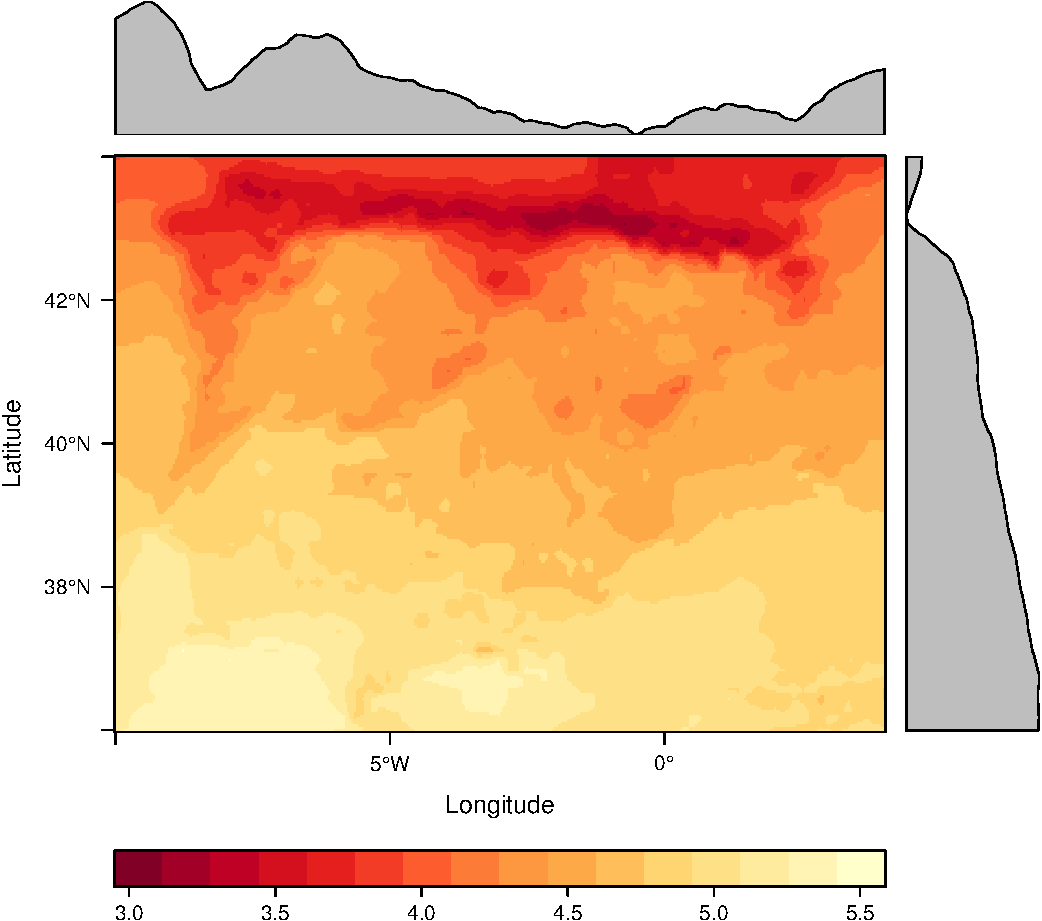
\includegraphics[width=.9\linewidth]{figs/leveplotSISavOrig.pdf}
\caption{\label{fig:levelplotCMSAF}Annual average of solar radiation displayed with a sequential palette.}
\end{figure}

Although the solar irradiation distribution reveals the physical
structure of the region, it is recommended to add the geographic
context with a layer of administrative boundaries (Figure
\ref{fig:levelplotCMSAF_boundaries}).

\index{Packages!maps@\texttt{maps}}
\index{Packages!mapdata@\texttt{mapdata}}
\index{Packages!maptools@\texttt{maptools}}
\index{map2SpatialLines@\texttt{map2SpatialLines}}

\lstset{language=R,numbers=none}
\begin{lstlisting}
library(maps)
library(mapdata)
library(maptools)

ext <- as.vector(extent(SISav))
boundaries <- map('worldHires',
		  xlim=ext[1:2], ylim=ext[3:4],
		  plot=FALSE)
boundaries <- map2SpatialLines(boundaries,
			       proj4string=CRS(projection(SISav)))
\end{lstlisting}

\index{Packages!sp@\texttt{sp}}
\index{Packages!latticeExtra@\texttt{latticeExtra}}
\index{sp.lines@\texttt{sp.lines}}

\lstset{language=R,numbers=none}
\begin{lstlisting}
levelplot(SISav) + layer(sp.lines(boundaries, lwd=0.5))
\end{lstlisting}

\begin{figure}[htb]
\centering
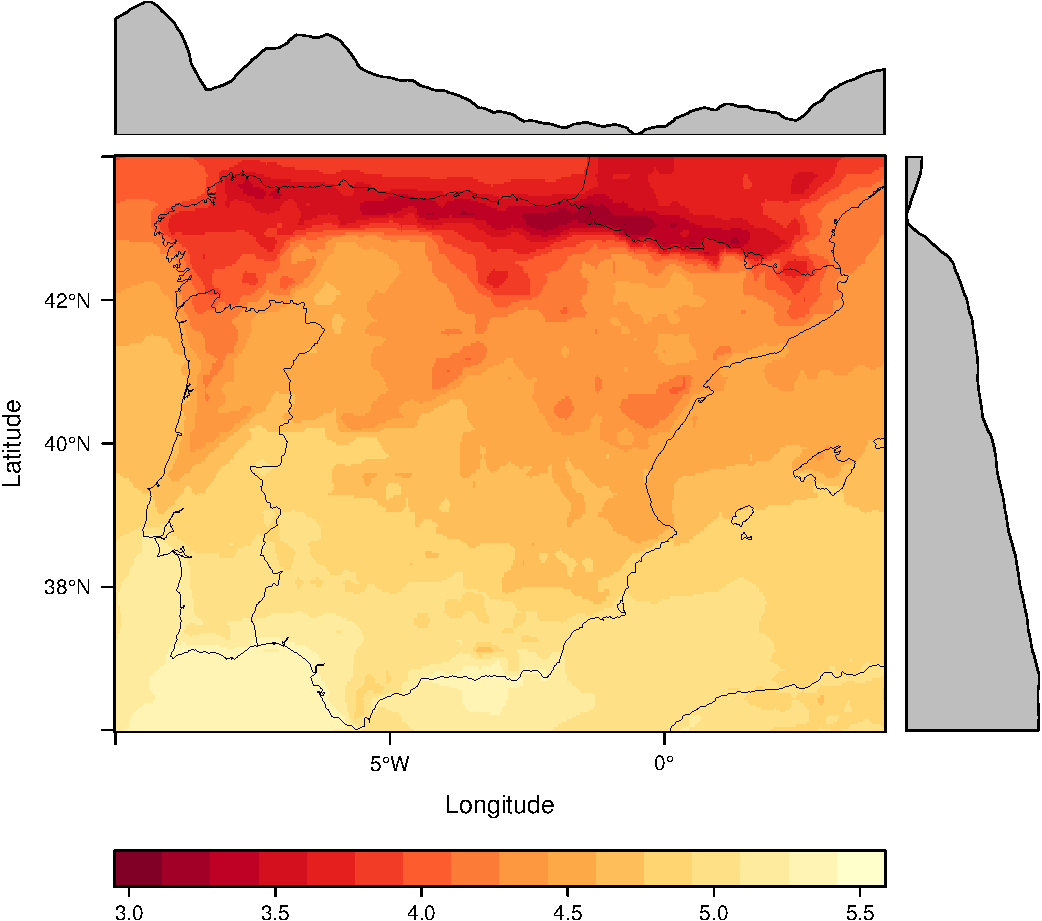
\includegraphics[width=.9\linewidth]{figs/leveplotSISavBoundaries.pdf}
\caption{\label{fig:levelplotCMSAF_boundaries}Annual average of solar radiation with administrative boundaries.}
\end{figure}

\subsubsection{Hill Shading}
\label{sec-1-1-1}
A frequent method to improve the display of meteorological rasters is
the hill shading or shaded relief technique, a method of representing
relief on a map by depicting the shadows that would be cast by high
ground if light comes from a certain sun position (Figure
\ref{fig:hillShading}).

The procedure is as follows:

\begin{itemize}
\item Download a Digital Elevation Model (DEM) from the DIVA-GIS service.
\end{itemize}
\index{Data!DIVA-GIS}

\lstset{language=R,numbers=none}
\begin{lstlisting}
old <- setwd(tempdir())
download.file('http://www.diva-gis.org/data/msk_alt/ESP_msk_alt.zip', 'ESP_msk_alt.zip')
unzip('ESP_msk_alt.zip', exdir='.')

DEM <- raster('ESP_msk_alt')
\end{lstlisting}

\begin{itemize}
\item Compute the hill shade raster with \texttt{terrain} and \texttt{hillShade} from \texttt{raster}.
\end{itemize}
\index{terrain@\texttt{terrain}}
\index{hillShade@\texttt{hillShade}}

\lstset{language=R,numbers=none}
\begin{lstlisting}
slope <- terrain(DEM, 'slope')
aspect <- terrain(DEM, 'aspect')
hs <- hillShade(slope=slope, aspect=aspect,
		angle=20, direction=30)
\end{lstlisting}
\lstset{language=R,numbers=none}
\begin{lstlisting}
setwd(old)
\end{lstlisting}

\begin{itemize}
\item Combine the result with the previous map using semitransparency.
\end{itemize}
\index{+.trellis@\texttt{+.trellis}}
\index{layer@\texttt{layer}}

\lstset{language=R,numbers=none}
\begin{lstlisting}
## hillShade theme: gray colors and semitransparency
hsTheme <- modifyList(GrTheme(), list(regions=list(alpha=0.6)))

levelplot(SISav, panel=panel.levelplot.raster,
	  margin=FALSE, colorkey=FALSE) +
    levelplot(hs, par.settings=hsTheme, maxpixels=1e6) +
    layer(sp.lines(boundaries, lwd=0.5))
\end{lstlisting}

\begin{figure}[htb]
\centering
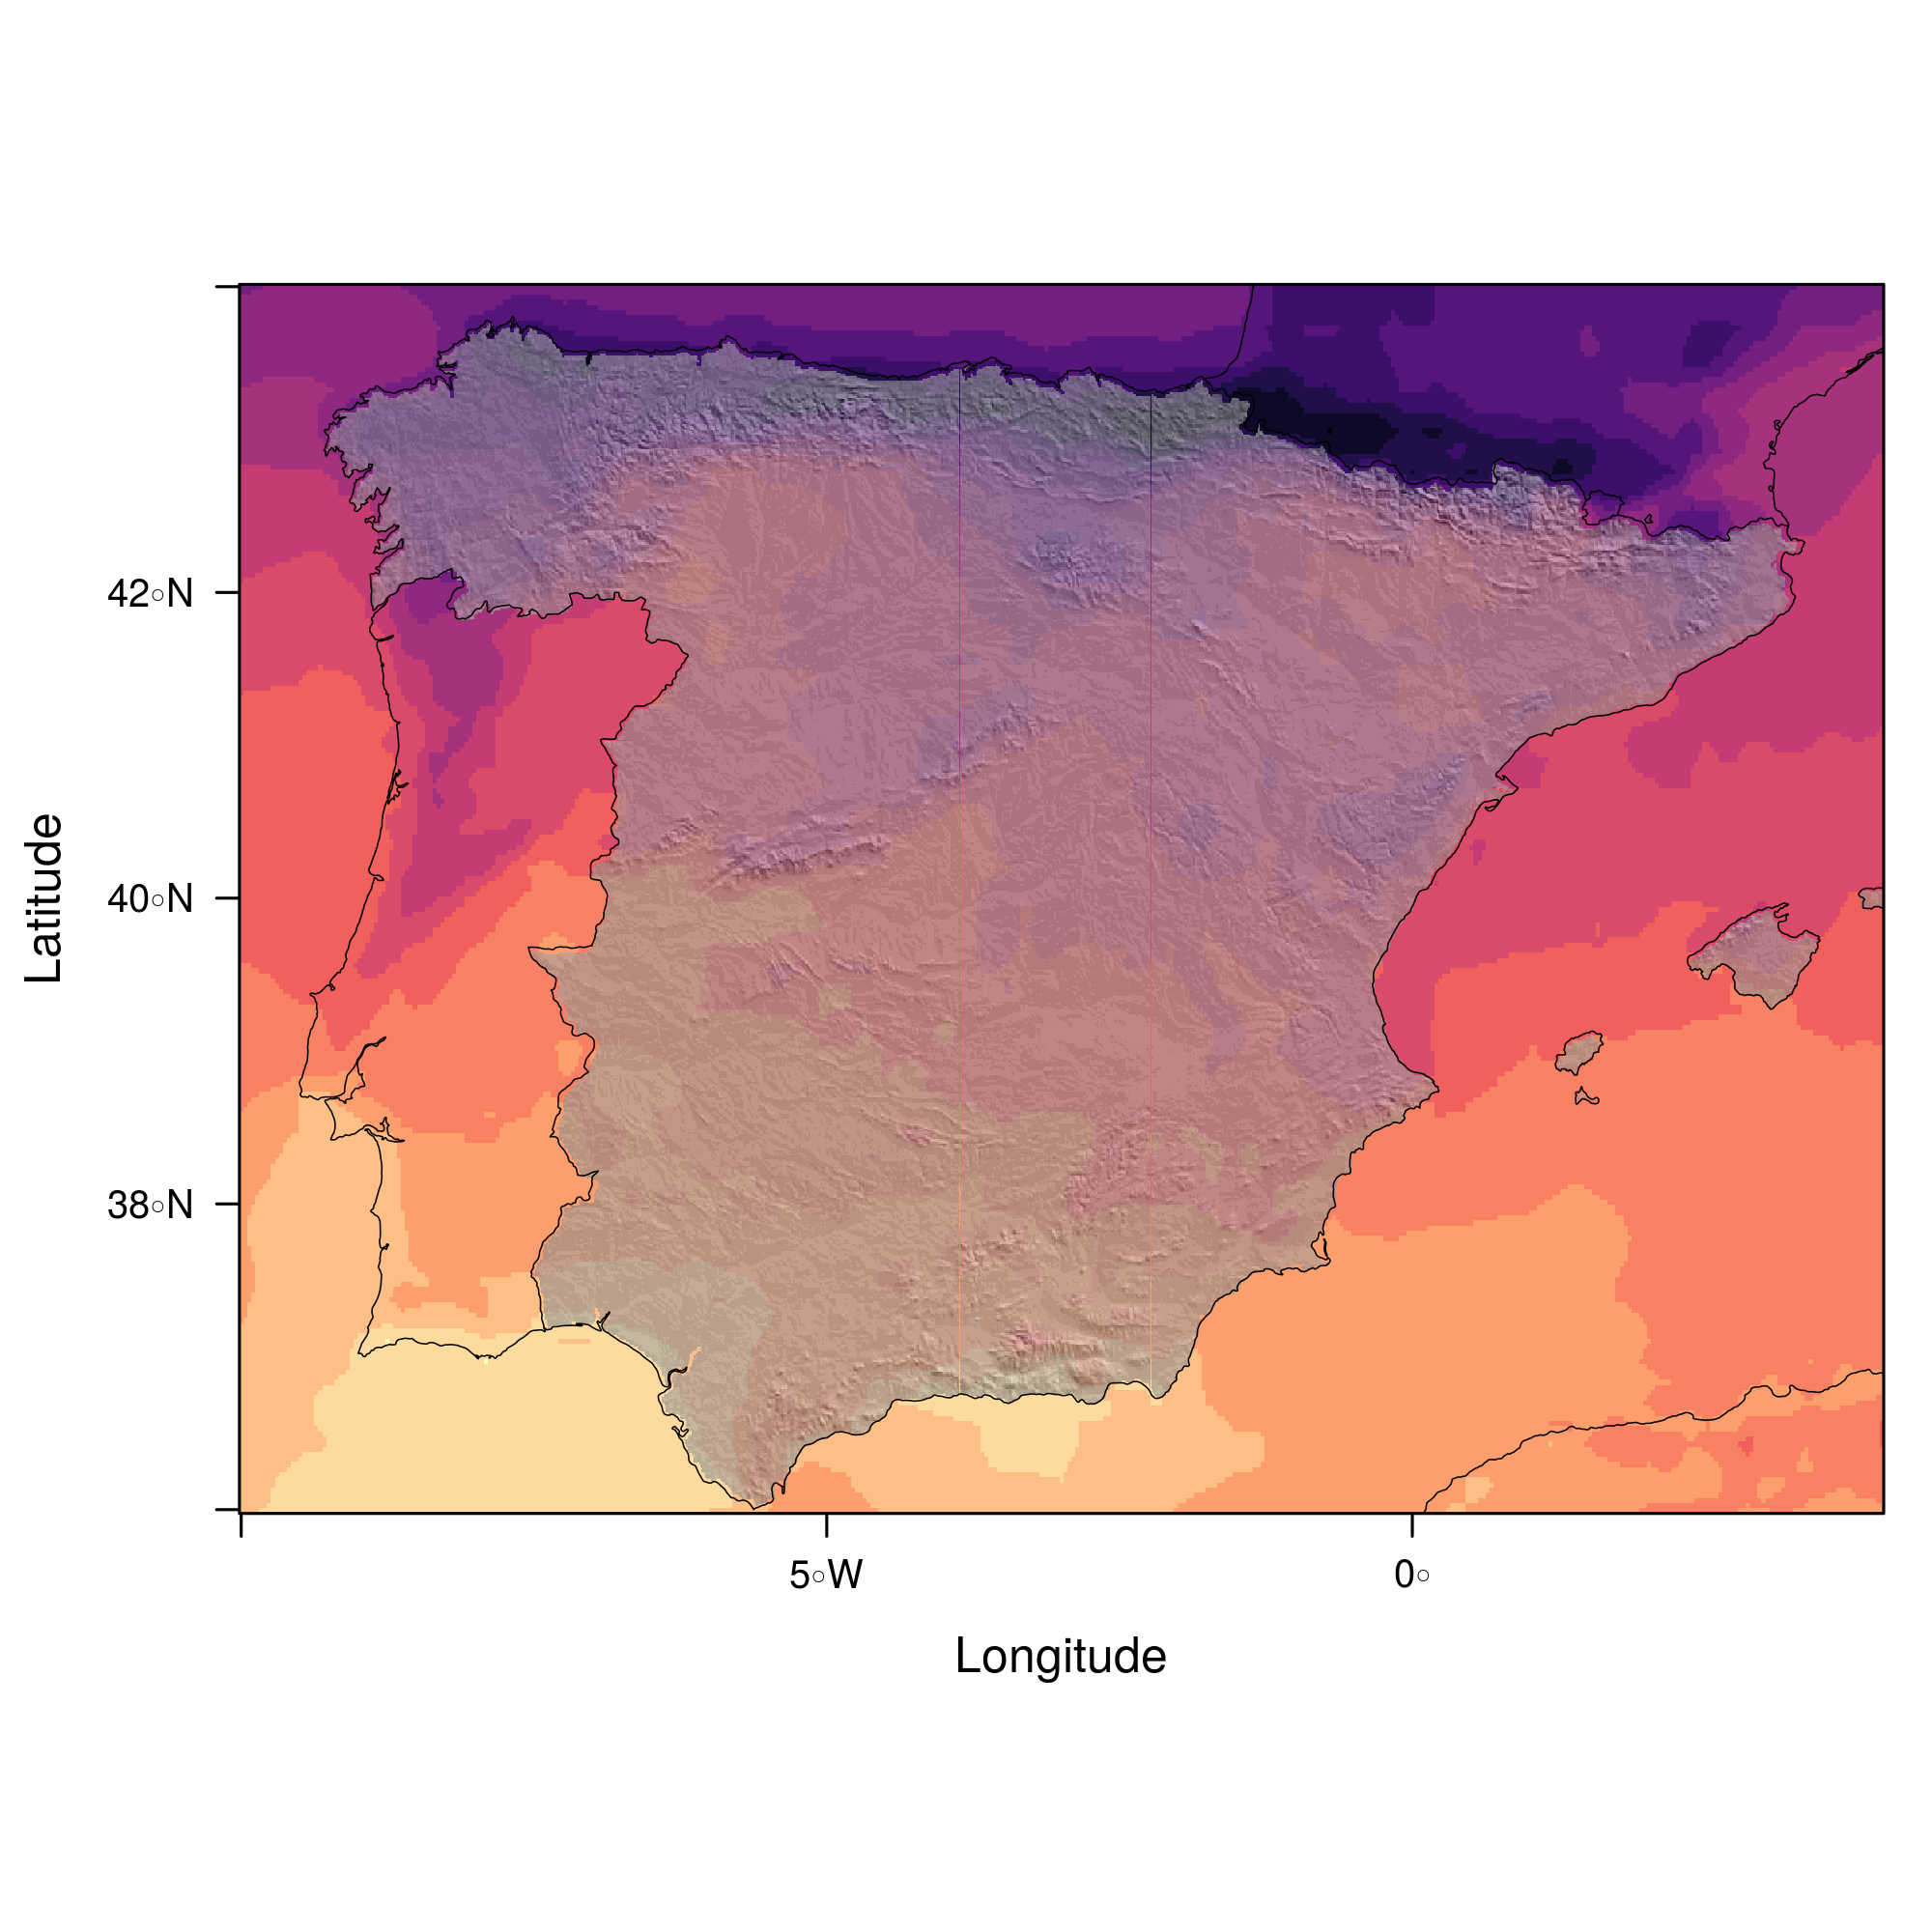
\includegraphics[width=.9\linewidth]{figs/hillShading.png}
\caption{\label{fig:hillShading}Hill shading of annual average of solar radiation.}
\end{figure}
\subsubsection{Excursus: 3D Visualization}
\label{sec-1-1-2}
An alternative method for a DEM is 3D visualization where the user can
rotate or zoom the figure. This solution is available thanks to the
\texttt{rgl} package, which provides functions for 3D interactive
graphics. The \texttt{plot3D} function in the \texttt{rasterVis} package is a
wrapper to this package for \texttt{RasterLayer} objects.

\index{Packages!rgl@\texttt{rgl}}
\index{3D visualization}
\index{WebGL}
\index{STL}

\lstset{language=R,numbers=none}
\begin{lstlisting}
plot3D(DEM, maxpixels=5e4)
\end{lstlisting}

The output scene can be exported to several formats such as WebGL with
\texttt{writeWebGL} to be rendered in a browser, or \texttt{STL} with \texttt{writeSTL}, a
format commonly used in 3D printing. Files using this format are
viewed easily on GitHub (Figure \ref{fig:DEM_STL})

\lstset{language=R,numbers=none}
\begin{lstlisting}
writeSTL('figs/DEM.stl')
\end{lstlisting}

\begin{figure}
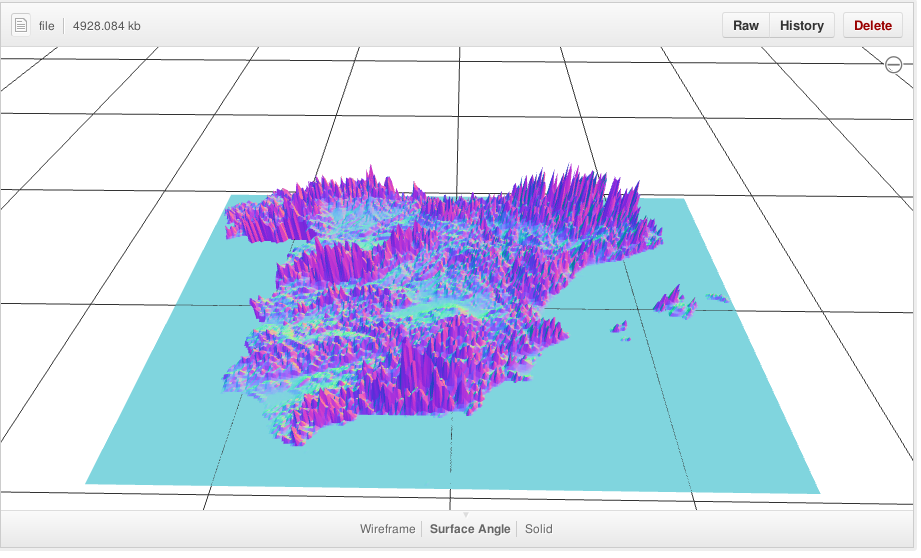
\includegraphics[height=0.3\textheight]{figs/DEM_STL_GitHub.png}
\caption{\label{fig:DEM_STL}3D visualization of a Digital Elevation
  Model using the STL format in a GitHub repository.}
\end{figure}

\subsubsection{Diverging Palettes}
\label{sec-1-1-3}
Next, instead of displaying the absolute values of each cell, we will
analyze the differences between each cell and the global average
value. This average is computed with the \texttt{cellStats} function and
substracted from the original \texttt{RasterLayer}. Figure
\ref{fig:xyplotSISav} displays the relation between these scaled
values and latitude (\texttt{y}), with five different groups defined by the
longitude (\texttt{cut(x, 5)}). It is evident that larger irradiation values
are associated with lower latitudes. However, there is no such clear
relation between irradiation and longitude.

\index{cellStats@\texttt{cellStats}}

\lstset{language=R,numbers=none}
\begin{lstlisting}
meanRad <- cellStats(SISav, 'mean')
SISav <- SISav - meanRad
\end{lstlisting}

\index{xyplot@\texttt{xyplot}}
\index{rasterTheme@\texttt{rasterTheme}}
\index{Packages!hexbin@\texttt{hexbin}}
\index{plinrain@\texttt{plinrain}}

\lstset{language=R,numbers=none}
\begin{lstlisting}
xyplot(layer ~ y, data = SISav,
       groups=cut(x, 5),
       par.settings=rasterTheme(symbol=plinrain(n=5, end=200)),
       xlab = 'Latitude', ylab = 'Solar radiation (scaled)',  
       auto.key=list(space='right', title='Longitude', cex.title=1.3))
\end{lstlisting}

\begin{figure}[htb]
\centering
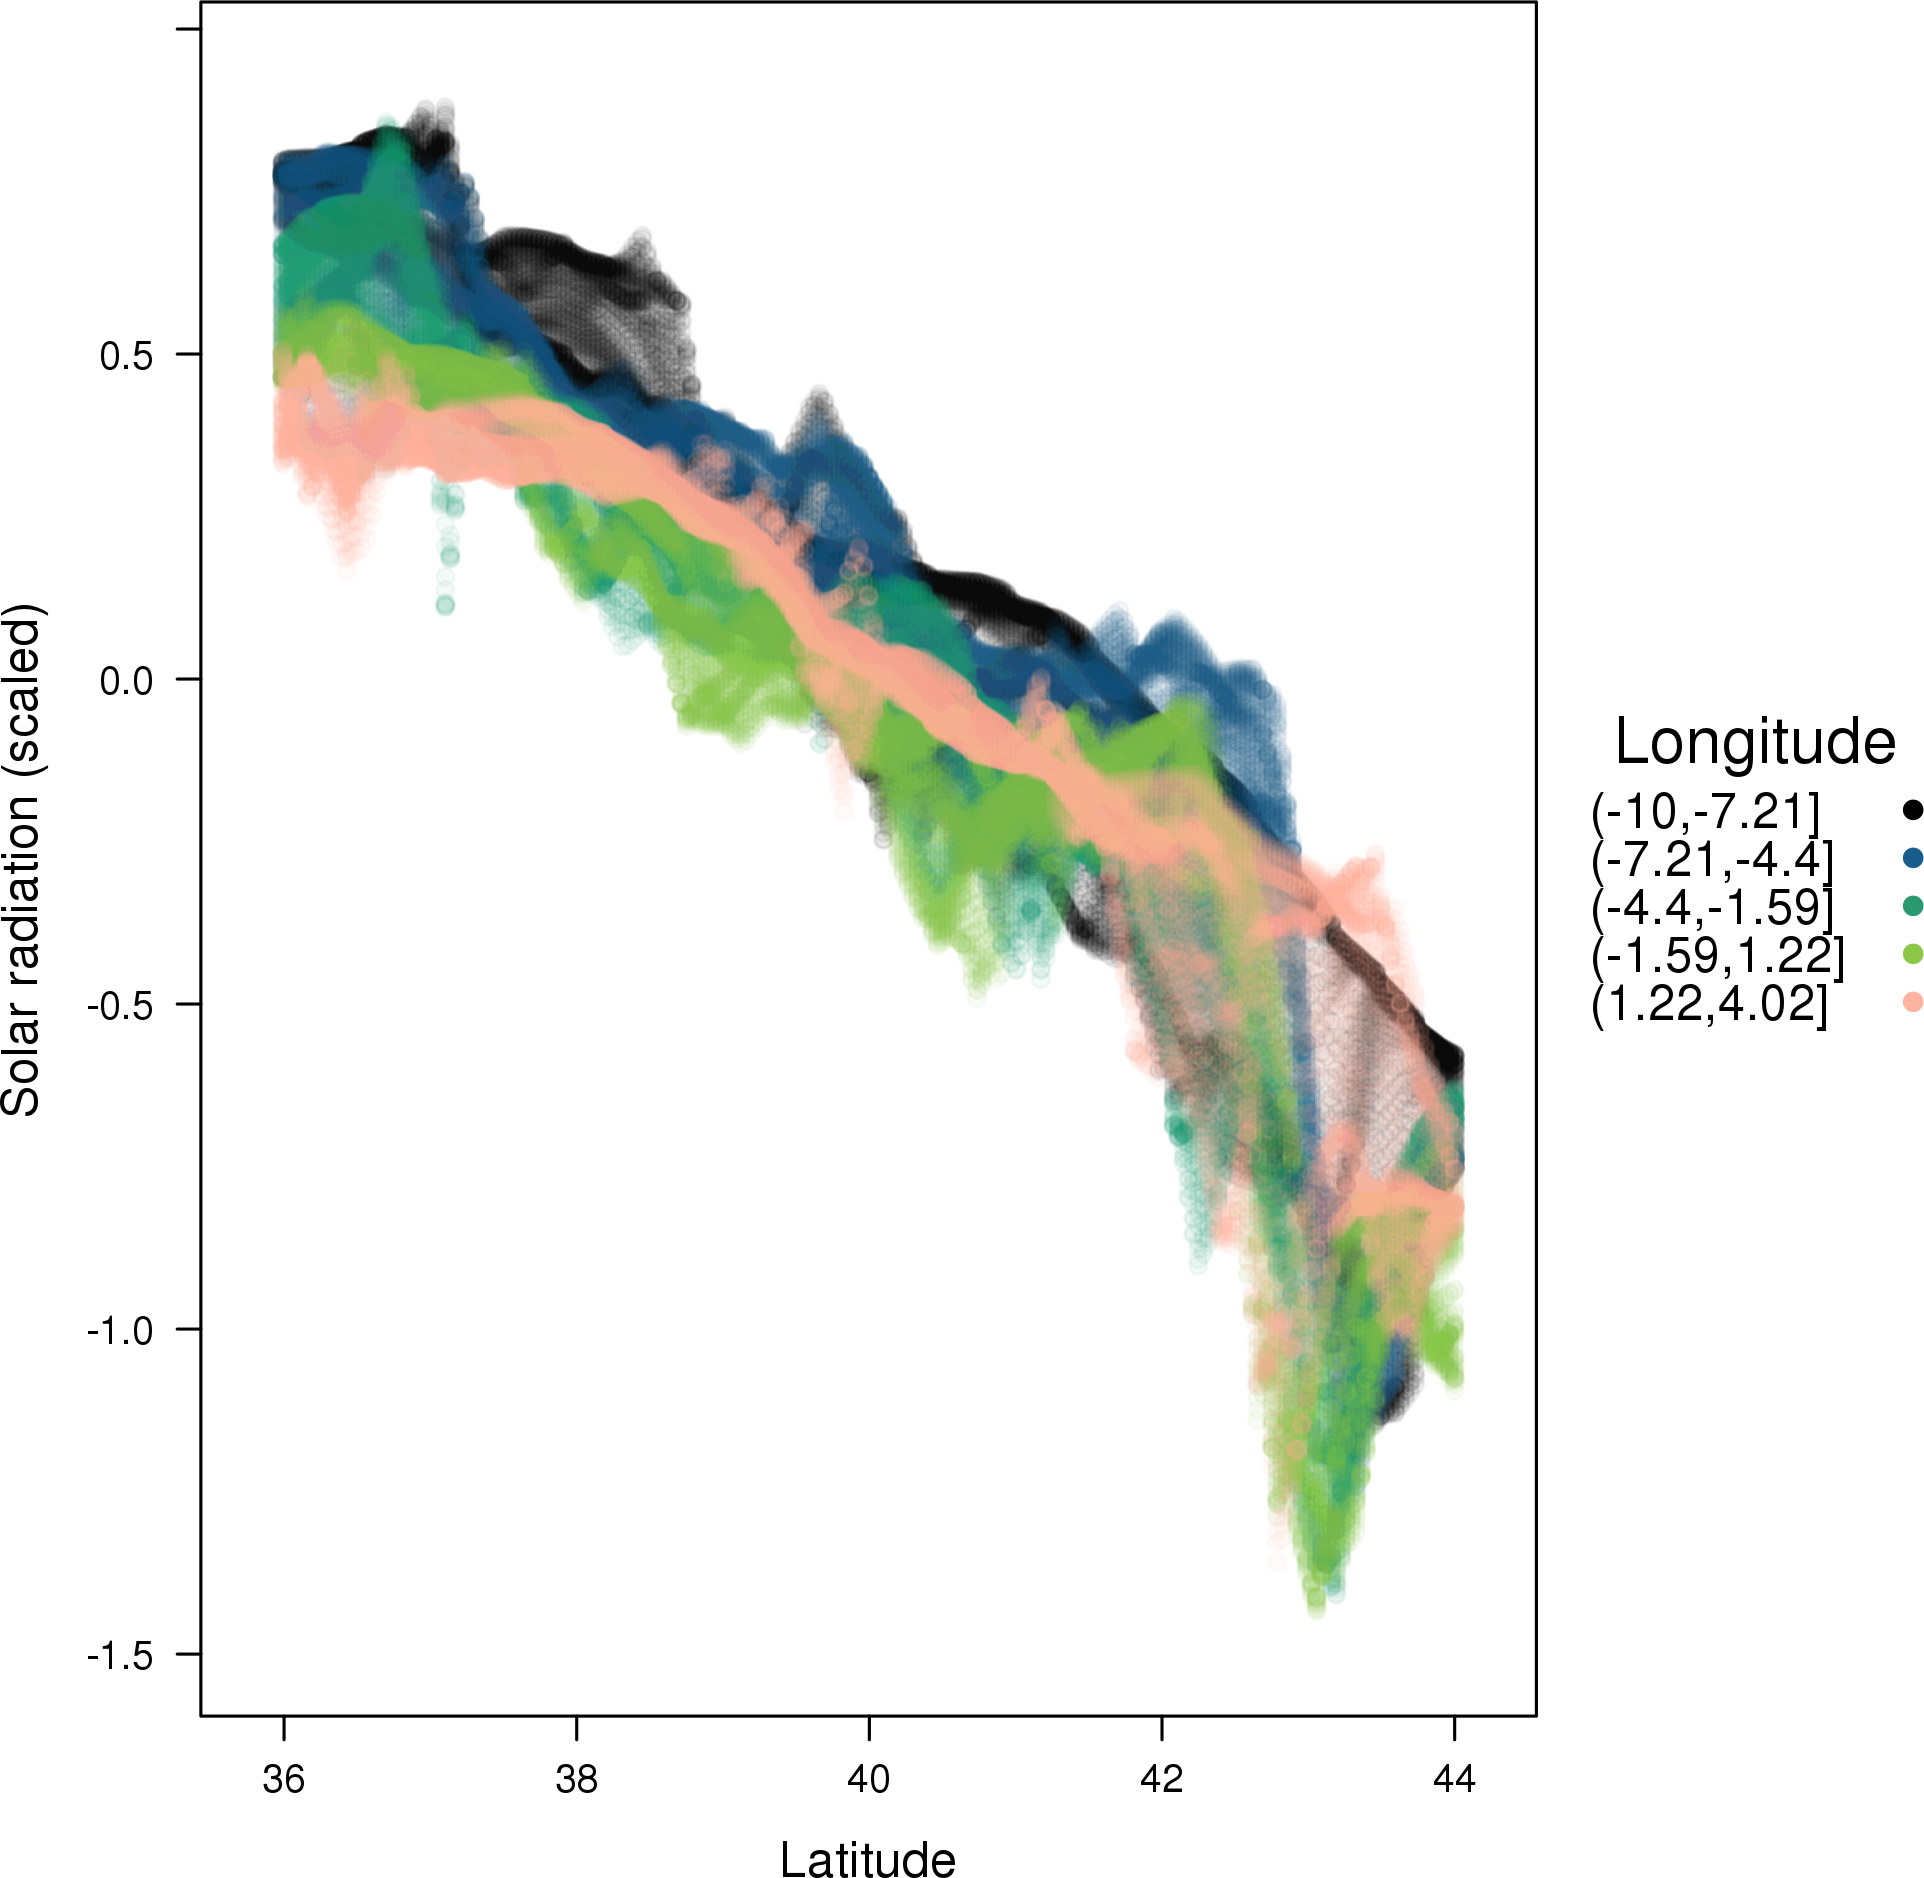
\includegraphics[width=.9\linewidth]{figs/xyplotSISav.png}
\caption{\label{fig:xyplotSISav}Relation between scaled annual average radiation and latitude for several longitude groups.}
\end{figure}

Numerical information ranging in an interval including a neutral
value is commonly displayed with diverging palettes. These
palettes represent neutral classes with light colors, while low
and high extremes of the data range are highlighted using dark
colors with contrasting hues. I use the Purple-Orange palette from
ColorBrewer with purple for positive values and orange for
negative values. In order to underline the position of the
interval containing zero, the center color of this palette is
substituted with pure white. The resulting palette is displayed in
Figure \ref{fig:showDivPal} with the custom \texttt{showPal}
function. The corresponding correspondent raster map produced with this palette
is displayed in Figure \ref{fig:divPal_SISav_naive}.  Although
extreme positive and negative values can be easily discriminated,
the zero value is not associated with white because the data range
is not symmetrical around zero.

\index{Package!RColorBrewer@\texttt{RColorBrewer}}
\index{brewer.pal@\texttt{brewer.pal}}

\lstset{language=R,numbers=none}
\begin{lstlisting}
divPal <- brewer.pal(n=9, 'PuOr')
divPal[5] <- "#FFFFFF"

showPal <- function(pal, labs=pal, cex=0.6, ...){
  barplot(rep(1, length(pal)), col=pal,
	  names.arg=labs, cex.names=cex,
	  axes=FALSE, ...)
}

showPal(divPal)
\end{lstlisting}

\begin{figure}[htb]
\centering
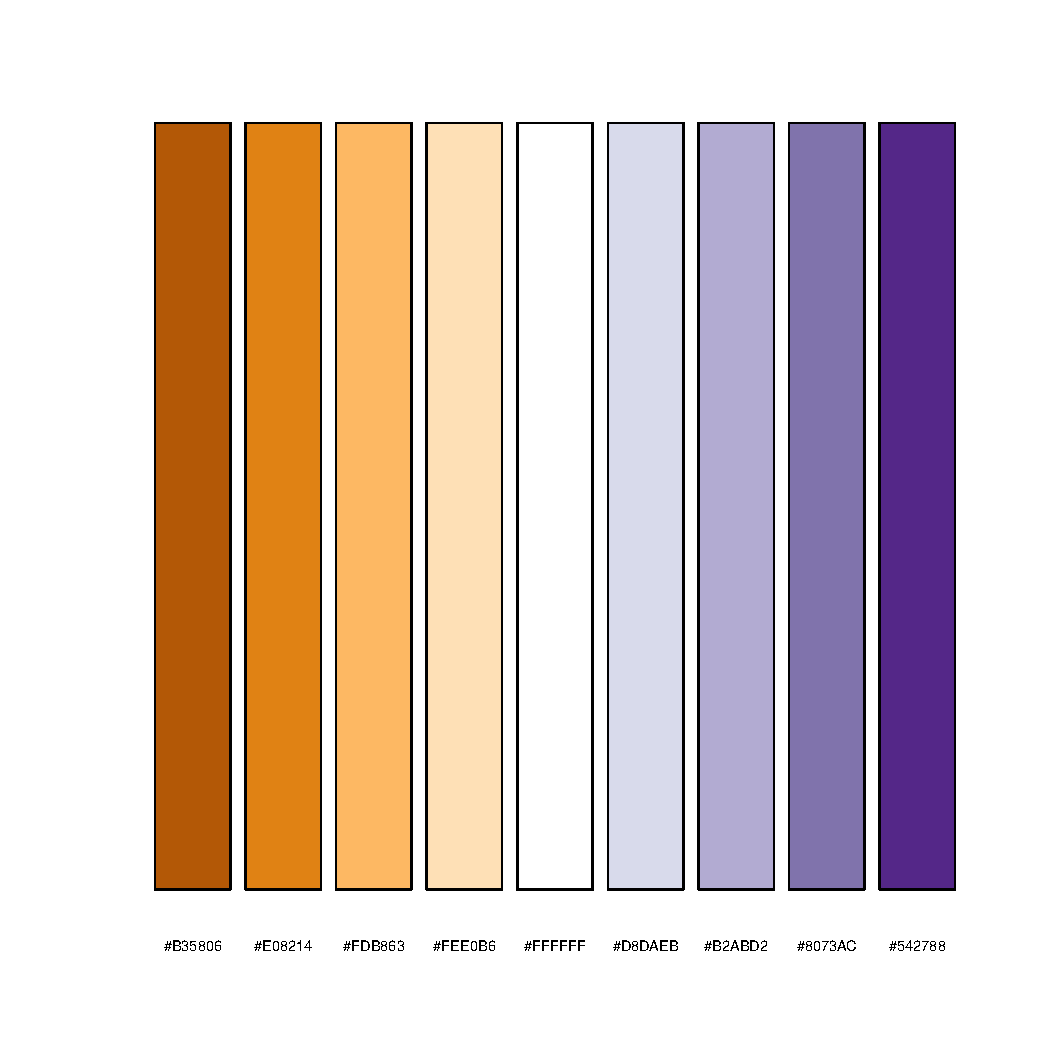
\includegraphics[height=0.3\textheight]{figs/showDivPal.pdf}
\caption{\label{fig:showDivPal}Purple-Orange diverging palette using white as middle color.}
\end{figure}


\lstset{language=R,numbers=none}
\begin{lstlisting}
divTheme <- rasterTheme(region=divPal)

levelplot(SISav, contour=TRUE, par.settings=divTheme)
\end{lstlisting}

\begin{figure}[htb]
\centering
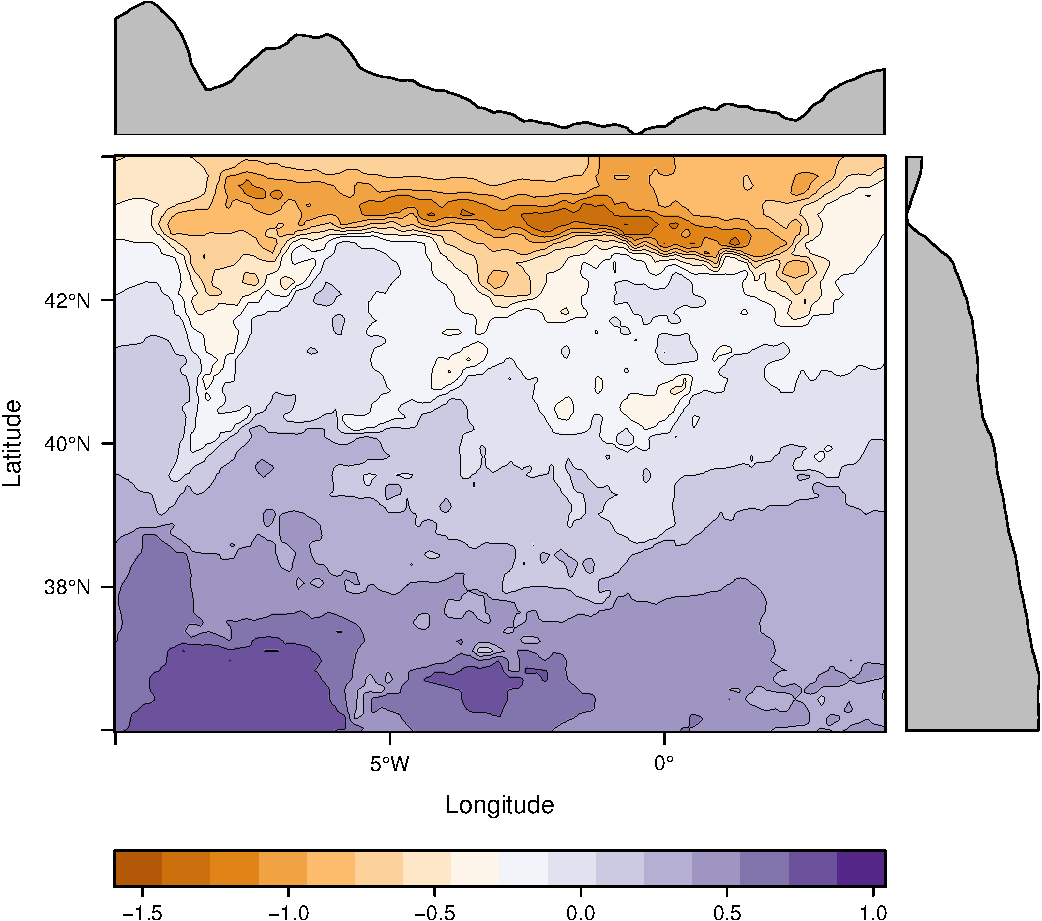
\includegraphics[width=.9\linewidth]{figs/divPal_SISav_naive.pdf}
\caption{\label{fig:divPal_SISav_naive}Asymmetric raster data (scaled annual average irradiation) displayed with a symmetric diverging palette.}
\end{figure}

The solution is to connect the symmetrical color palette with the
asymmetrical data range. The first step is to create a set of
breaks such that the zero value is the center of one of the
intervals.
\lstset{language=R,numbers=none}
\begin{lstlisting}
rng <- range(SISav[])
## Number of desired intervals
nInt <- 15
## Increment corresponding to the range and nInt
inc0 <- diff(rng)/nInt
## Number of intervals from the negative extreme to zero
n0 <- floor(abs(rng[1])/inc0)
## Update the increment adding 1/2 to position zero in the center of an interval
inc <- abs(rng[1])/(n0 + 1/2)
## Number of intervals from zero to the positive extreme
n1 <- ceiling((rng[2]/inc - 1/2) + 1)
## Collection of breaks
breaks <- seq(rng[1], by=inc, length= n0 + 1 + n1)
\end{lstlisting}

The next step is to compute the midpoints of each interval. These
points represent the data belonging to each interval, and their value
will be connected with a color of the palette.
\index{findInterval@\texttt{findInterval}}
\index{tapply@\texttt{tapply}}

\lstset{language=R,numbers=none}
\begin{lstlisting}
## Midpoints computed with the median of each interval
idx <- findInterval(SISav[], breaks, rightmost.closed=TRUE)
mids <- tapply(SISav[], idx, median)
## Maximum of the absolute value both limits
mx <- max(abs(breaks))
mids
\end{lstlisting}

A simple method to relate the palette and the intervals is with a
straight line such that a point is defined by the absolute maximum
value, (\texttt{(mx, 1)}), and another point by zero, (\texttt{(0, 0.5)}).  Why are
we using the interval [0, 1] as the \texttt{y}-coordinate of this line, and
why is 0.5 the result of zero? The reason is that the input of the
\texttt{break2pal} function will be the result of \texttt{colorRamp}, a function
that creates another interpolating function which maps colors with
values between 0 and 1. Therefore, a new palette is created,
extracting colors from the original palette, such that the central
color (white) is associated with the interval containing zero. This
palette is displayed in Figure \ref{fig:showBreak2Pal}.

The raster map produced with this new palette is displayed in Figure
\ref{fig:divPalSISav}. Now zero is clearly associated with the white
color.
\index{colorRamp@\texttt{colorRamp}}
\index{rgb@\texttt{rgb}}
\lstset{language=R,numbers=none}
\begin{lstlisting}
break2pal <- function(x, mx, pal){
  ## x = mx gives y = 1
  ## x = 0 gives y = 0.5
  y <- 1/2*(x/mx + 1)
  rgb(pal(y), maxColorValue=255)
}

## Interpolating function that maps colors with [0, 1]
## rgb(divRamp(0.5), maxColorValue=255) gives "#FFFFFF" (white)
divRamp <- colorRamp(divPal)
## Diverging palette where white is associated with the interval
## containing the zero
pal <- break2pal(mids, mx, divRamp)
showPal(pal, round(mids, 1))
\end{lstlisting}

\begin{figure}[htb]
\centering
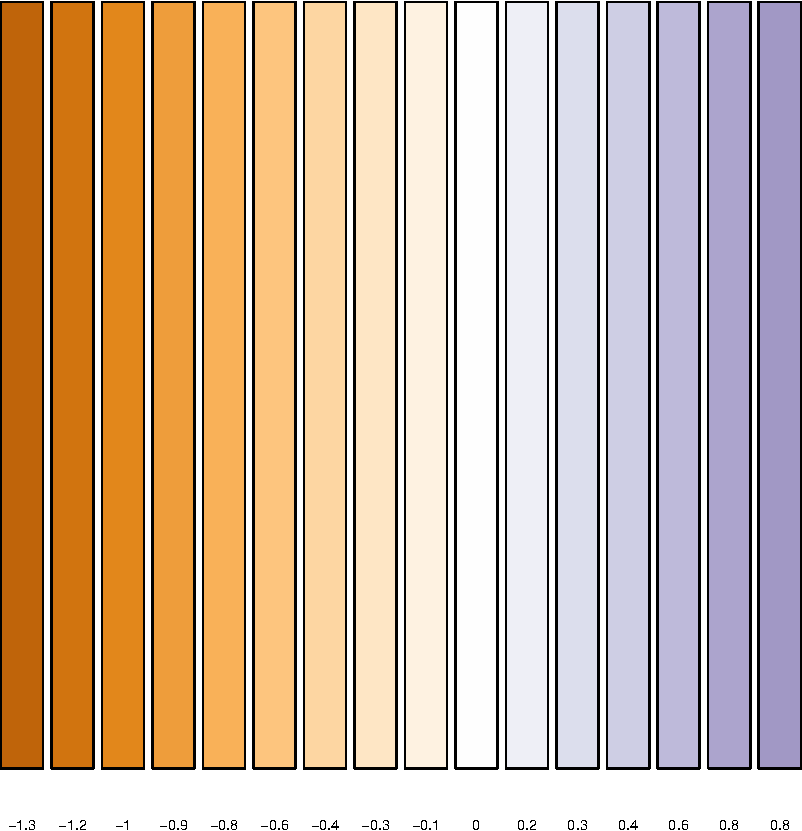
\includegraphics[height=0.3\textheight]{figs/showBreak2Pal.pdf}
\caption{\label{fig:showBreak2Pal}Modified diverging palette related with the asymmetrical raster data.}
\end{figure}


\lstset{language=R,numbers=none}
\begin{lstlisting}
levelplot(SISav, par.settings=rasterTheme(region=pal),
	  at=breaks, contour=TRUE)
\end{lstlisting}

\begin{figure}[htb]
\centering
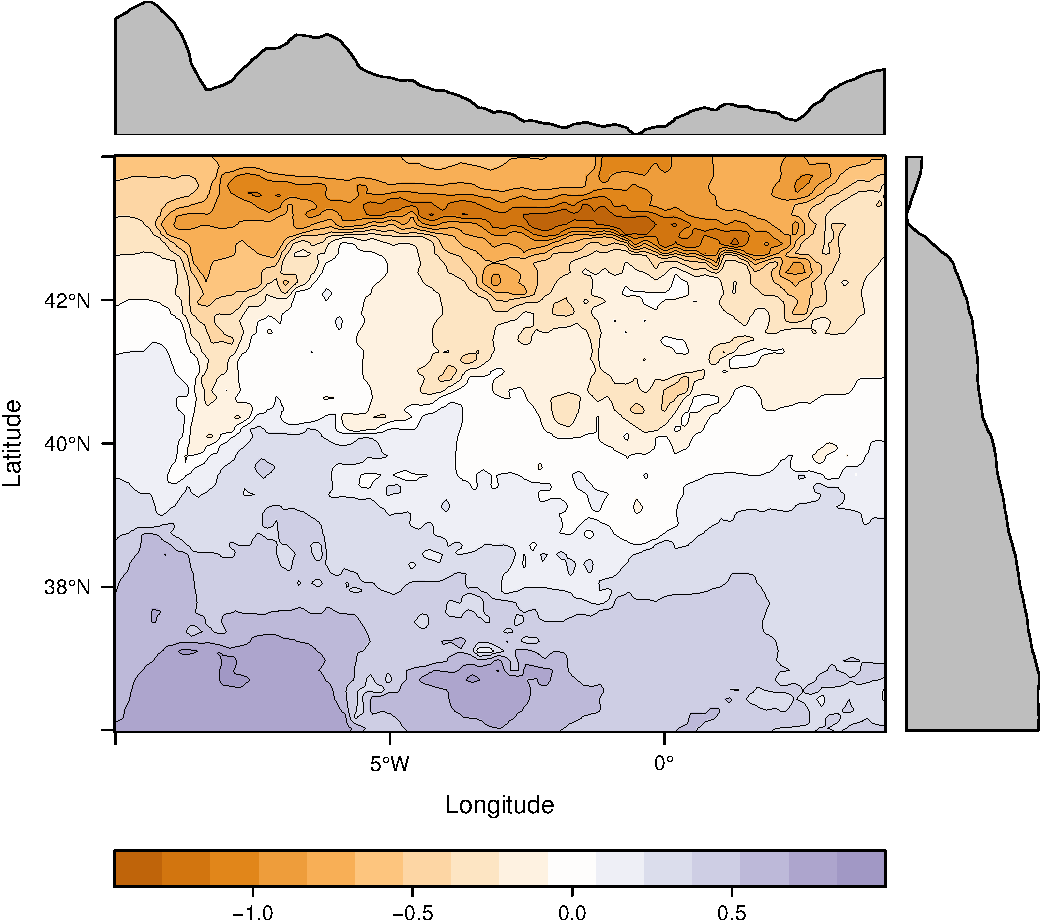
\includegraphics[width=.9\linewidth]{figs/divPalSISav.pdf}
\caption{\label{fig:divPalSISav}Asymmetric raster data (scaled annual average irradiation) displayed with a modified diverging palette.}
\end{figure}


It is interesting to note two operations carried out internally by
the \texttt{lattice} package. First, the \texttt{custom.theme} function (used by
\texttt{rasterTheme}) creates a new palette with 100 colors using
\texttt{colorRampPalette} to interpolate the palette passed as an
argument. Second, the \texttt{level.colors} function makes the
arrangement between intervals and colors. If this function
receives more colors than intervals, it chooses a subset of the
palette disregarding some of the intermediate colors. Therefore,
because this function will receive 100 colors from \texttt{par.settings}, it
is difficult to control exactly which colors of our original
palette will be represented.

An alternative way for finer control is to fill the \texttt{regions\$col}
component of the theme with our palette after it has been created
(Figure \ref{fig:divPal_SISav_regions}).

\lstset{language=R,numbers=none}
\begin{lstlisting}
divTheme <- rasterTheme()

divTheme$regions$col <- pal
levelplot(SISav, par.settings=divTheme, at=breaks, contour=TRUE)
\end{lstlisting}

\begin{figure}[htb]
\centering
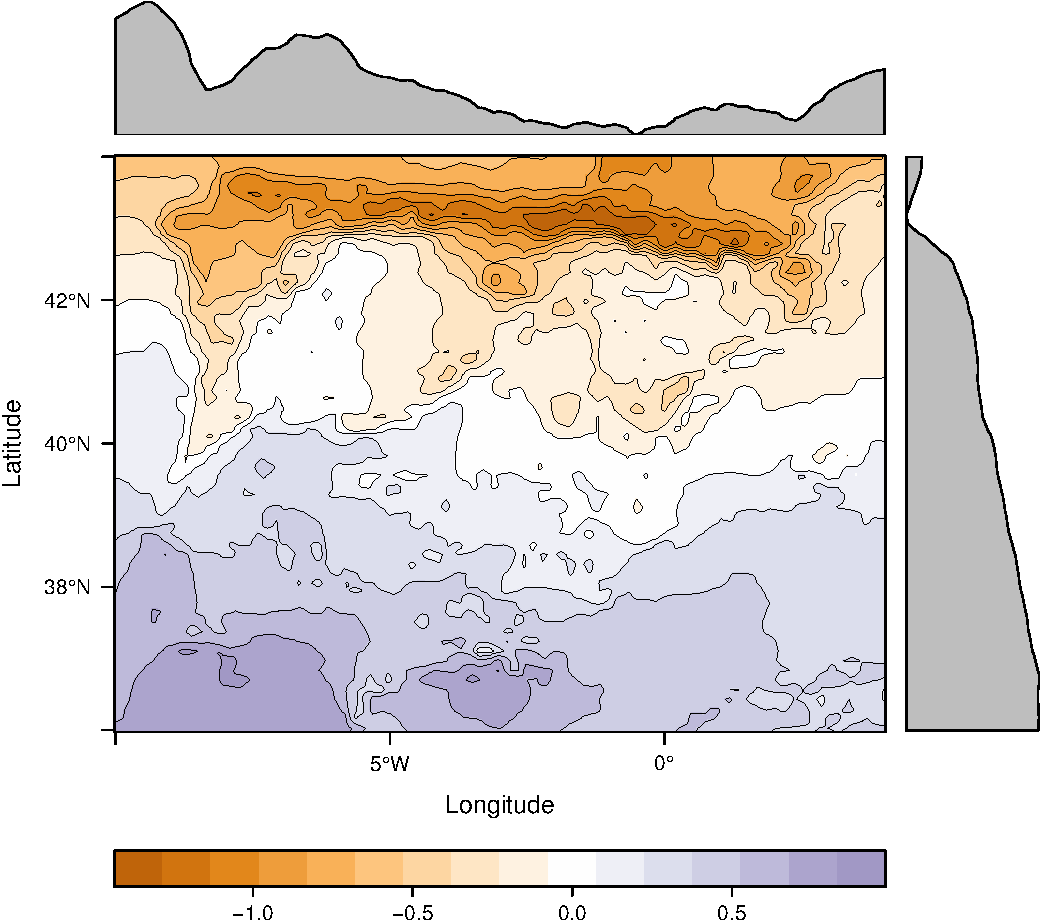
\includegraphics[width=.9\linewidth]{figs/divPalSISav_regions.pdf}
\caption{\label{fig:divPal_SISav_regions}Same as Figure \ref{fig:divPalSISav} but colors are assigned directly to the \texttt{regions\$col} component of the theme.}
\end{figure}

A final improvement to this map is to compute the intervals using a
classification algorithm with the \texttt{classInt} package. With this
approach it is likely that zero will not be perfectly centered in its
corresponding interval. The remaining code is exactly the same as
above, replacing the \texttt{breaks} vector with the result of the
\texttt{classIntervals} function. Figure \ref{fig:divPalSISav_classInt}
displays the result.

\index{Packages!classInt@\texttt{classInt}}
\index{classIntervals@\texttt{classIntervals}}

\lstset{language=R,numbers=none}
\begin{lstlisting}
library(classInt)

cl <- classIntervals(SISav[],
		     ## n=15, style='equal')
		     ## style='hclust')
		     ## style='sd')
		     style='kmeans')
		     ## style='quantile')
cl
breaks <- cl$brks
\end{lstlisting}

\lstset{language=R,numbers=none}
\begin{lstlisting}
idx <- findInterval(SISav[], breaks, rightmost.closed=TRUE)
mids <- tapply(SISav[], idx, median)
mids
mx <- max(abs(breaks))
pal <- break2pal(mids, mx, divRamp)
divTheme$regions$col <- pal
levelplot(SISav, par.settings=divTheme, at=breaks, contour=TRUE)
\end{lstlisting}

\begin{figure}[htb]
\centering
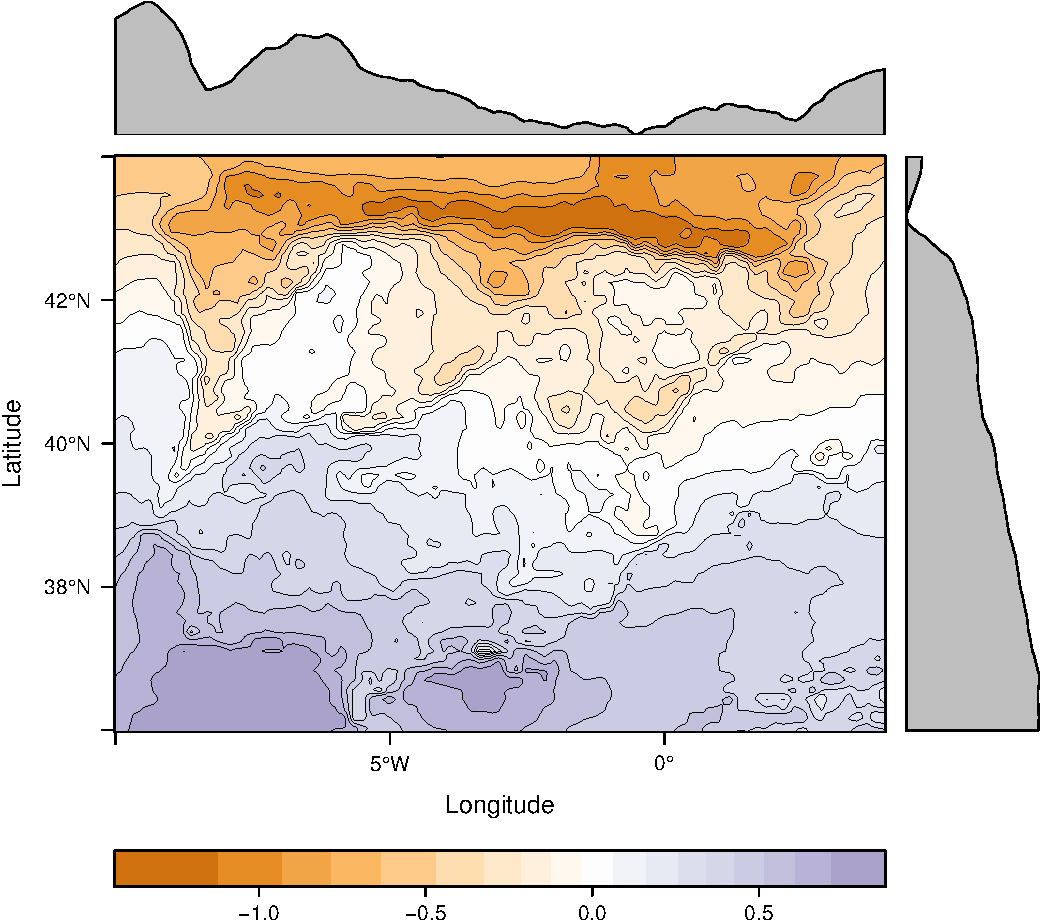
\includegraphics[width=.9\linewidth]{figs/divPalSISav_classInt.pdf}
\caption{\label{fig:divPalSISav_classInt}Same as Figure \ref{fig:divPal_SISav_regions} but defining intervals with the optimal classification method.}
\end{figure}

\subsection{Categorical Data}
\label{sec-1-2}
Land cover is the observed physical cover on the Earth's surface. A
set of seventeen different categories is commonly used. Using
satellite observations, it is possible to map where on Earth each of
these seventeen land surface categories can be found and how these
land covers change over time.

This section illustrates how to read and display rasters with
categorical information using information from the NEO-NASA
project. After the land cover and population density files have been
downloaded, two \texttt{RasterLayers} can be created with the \texttt{raster}
package. Both files are read, their geographical extent reduced to the
area of India and China, and cleaned (\texttt{99999} cells are replaced with
\texttt{NA}).

\index{Packages!raster@\texttt{raster}}
\index{extent@\texttt{extent}}
\index{crop@\texttt{crop}}

\lstset{language=R,numbers=none}
\begin{lstlisting}
library(raster)
## China and India  
ext <- extent(65, 135, 5, 55)

pop <- raster('875430rgb-167772161.0.FLOAT.TIFF')
pop <- crop(pop, ext)
pop[pop==99999] <- NA

landClass <- raster('241243rgb-167772161.0.TIFF')
landClass <- crop(landClass, ext)
\end{lstlisting}

Each land cover type is designated with a different key: the sea is
labeled with 0; forests with 1 to 5; shrublands, grasslands, and
wetlands with 6 to 11; agriculture and urban lands with 12 to 14; and
snow and barren with 15 and 16.  These four groups (sea is replaced by
\texttt{NA}) will be the levels of the categorical raster. The \texttt{raster}
package includes the \texttt{ratify} method to define a layer as categorical
data, filling it with integer values associated to a Raster Attribute
Table (RAT).


\index{ratify@\texttt{ratify}}
\index{cut@\texttt{cut}}

\lstset{language=R,numbers=none}
\begin{lstlisting}
landClass[landClass %in% c(0, 254)] <- NA
## Only four groups are needed:
## Forests: 1:5
## Shrublands, etc: 6:11
## Agricultural/Urban: 12:14
## Snow: 15:16
landClass <- cut(landClass, c(0, 5, 11, 14, 16))
## Add a Raster Attribute Table and define the raster as categorical data
landClass <- ratify(landClass)
## Configure the RAT: first create a RAT data.frame using the
## levels method; second, set the values for each class (to be
## used by levelplot); third, assign this RAT to the raster
## using again levels
rat <- levels(landClass)[[1]]
rat$classes <- c('Forest', 'Land', 'Urban', 'Snow')
levels(landClass) <- rat
\end{lstlisting}

This categorical raster can be displayed with the \texttt{levelplot} method
of the \texttt{rasterVis} package. Previously, a theme is defined with the
background color set to \texttt{lightskyblue1} to display the sea areas
(filled with \texttt{NA} values), and the region palette is defined with
adequate colors (Figure \ref{fig:landClass}).

\index{Packages!rasterVis@\texttt{rasterVis}}
\index{levelplot@\texttt{levelplot}}
\index{modifyList@\texttt{modifyList}}
\index{rasterTheme@\texttt{rasterTheme}}

\lstset{language=R,numbers=none}
\begin{lstlisting}
library(rasterVis)

pal <- c('palegreen4', # Forest
	 'lightgoldenrod', # Land
	 'indianred4', # Urban
	 'snow3')      # Snow

catTheme <- modifyList(rasterTheme(),
		       list(panel.background = list(col='lightskyblue1'),
			    regions = list(col= pal)))

levelplot(landClass, maxpixels=3.5e5, par.settings=catTheme,
	  panel=panel.levelplot.raster)
\end{lstlisting}

\begin{figure}[htb]
\centering
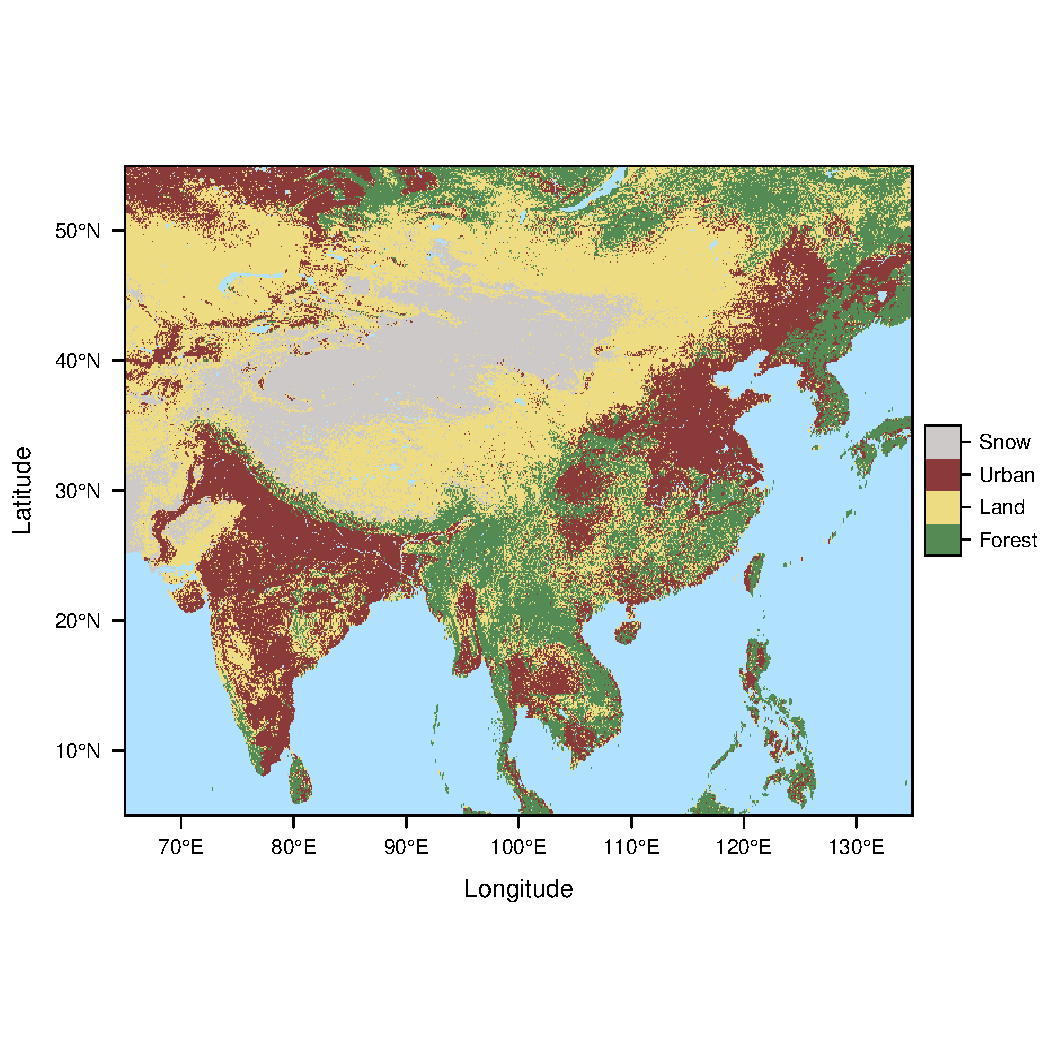
\includegraphics[width=.9\linewidth]{figs/landClass.pdf}
\caption{\label{fig:landClass}Land cover raster (categorical data).}
\end{figure}

Let's explore the relation between the land cover and population
density rasters. Figure \ref{fig:populationNASA} displays this
latter raster using a logarithmic scale.

\lstset{language=R,numbers=none}
\begin{lstlisting}
pPop <- levelplot(pop, zscaleLog=10, par.settings=BTCTheme,
		  maxpixels=3.5e5, panel=panel.levelplot.raster)
pPop
\end{lstlisting}

\begin{figure}[htb]
\centering
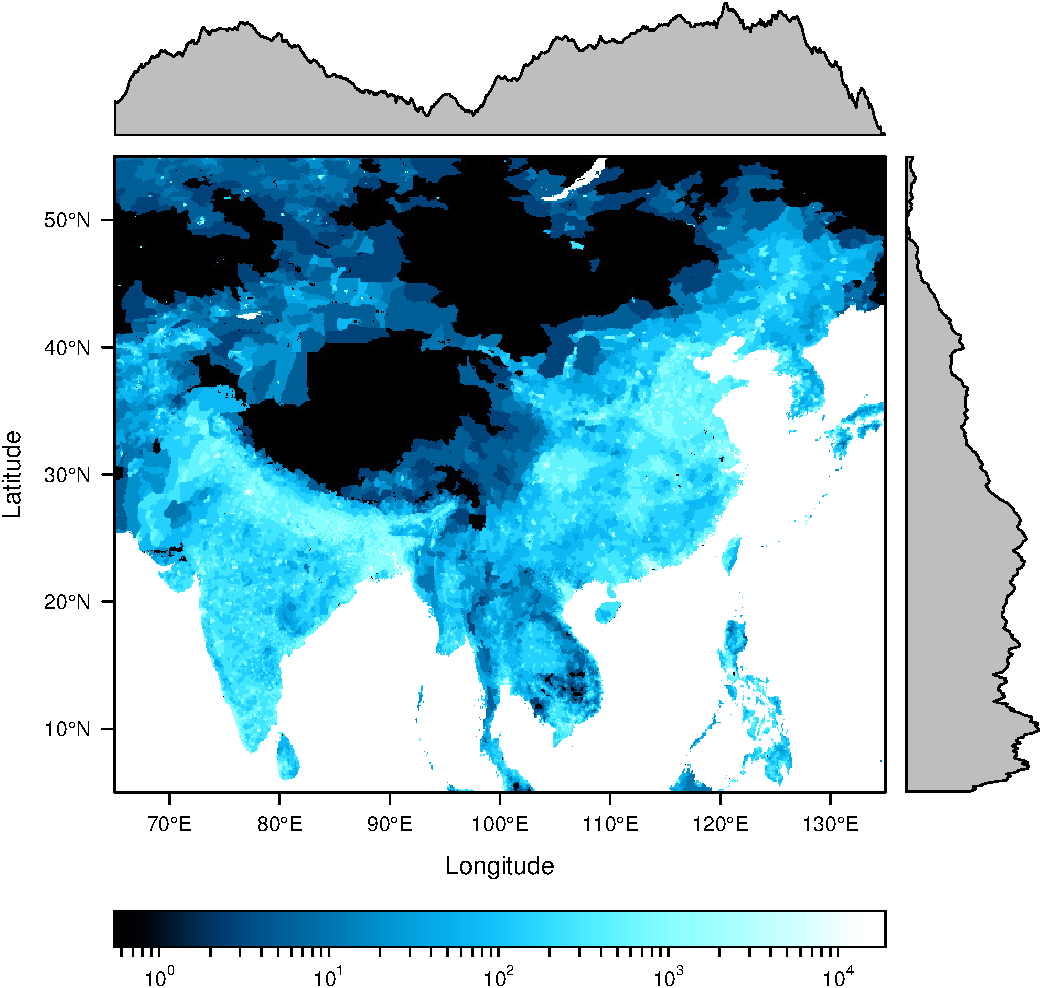
\includegraphics[width=.9\linewidth]{figs/populationNASA.pdf}
\caption{\label{fig:populationNASA}Population density raster.}
\end{figure}

Both rasters can be joined together with the \texttt{stack} method to
create a new \texttt{RasterStack} object. Figure
\ref{fig:histogramLandClass} displays the distribution of the
logarithm of the population density associated to each land class.

\index{stack@\texttt{stack}}
\index{histogram@\texttt{histogram}}

\lstset{language=R,numbers=none}
\begin{lstlisting}
s <- stack(pop, landClass)
names(s) <- c('pop', 'landClass')
histogram(~log10(pop)|landClass, data=s,
	  scales=list(relation='free'))
\end{lstlisting}

\begin{figure}[htb]
\centering
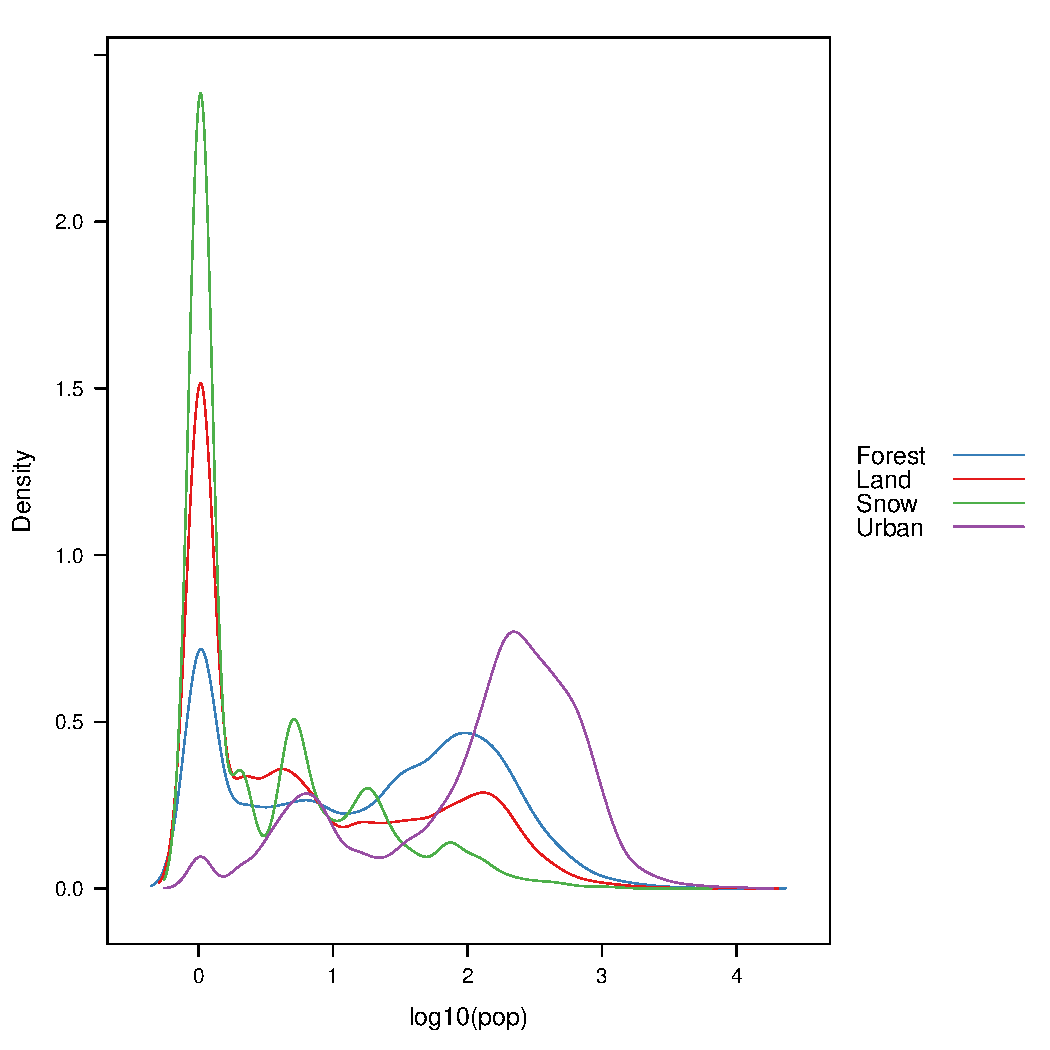
\includegraphics[width=.9\linewidth]{figs/histogramLandClass.pdf}
\caption{\label{fig:histogramLandClass}Distribution of the logarithm of the population density associated to each land class.}
\end{figure}

\subsection{\floweroneleft  Multivariate Legend}
\label{sec-1-3}
We can reproduce the code used to create the multivariate
choropleth (Section \ref{sec:multiChoropleth}) using the
\texttt{levelplot} function from the \texttt{rasterVis} package. Again, the
result is a list of \texttt{trellis} objects. Each of these objects is
the representation of the population density in a particular land
class. The \texttt{+.trellis} function of the \texttt{latticeExtra} package with
\texttt{Reduce} superposes the elements of this list and produces a
\texttt{trellis} object. Figure \ref{fig:popLandClass} displays the
result.




\lstset{language=R,numbers=none}
\begin{lstlisting}
library(colorspace)
## at for each sub-levelplot is obtained from the global levelplot
at <- pPop$legend$bottom$args$key$at
classes <- rat$classes
nClasses <- length(classes)

pList <- lapply(1:nClasses, function(i){
  landSub <- landClass
  ## Those cells from a different land class are set to NA...
  landSub[!(landClass==i)] <- NA
  ## ... and the resulting raster masks the population raster
  popSub <- mask(pop, landSub)
  ## The HCL color wheel is divided in nClasses
  step <- 360/nClasses
  ## and a sequential palette is constructed with a hue from one of
  ## the color wheel parts
  cols <- rev(sequential_hcl(16, h = (30 + step*(i-1))%%360))

  pClass <- levelplot(popSub, zscaleLog=10, at=at,
		      maxpixels=3.5e5,
		      ## labels only needed in the last legend
		      colorkey=(if (i==nClasses) TRUE else list(labels=list(labels=rep('', 17)))),
		      col.regions=cols, margin=FALSE)
})
\end{lstlisting}


\begin{figure}[htb]
\centering
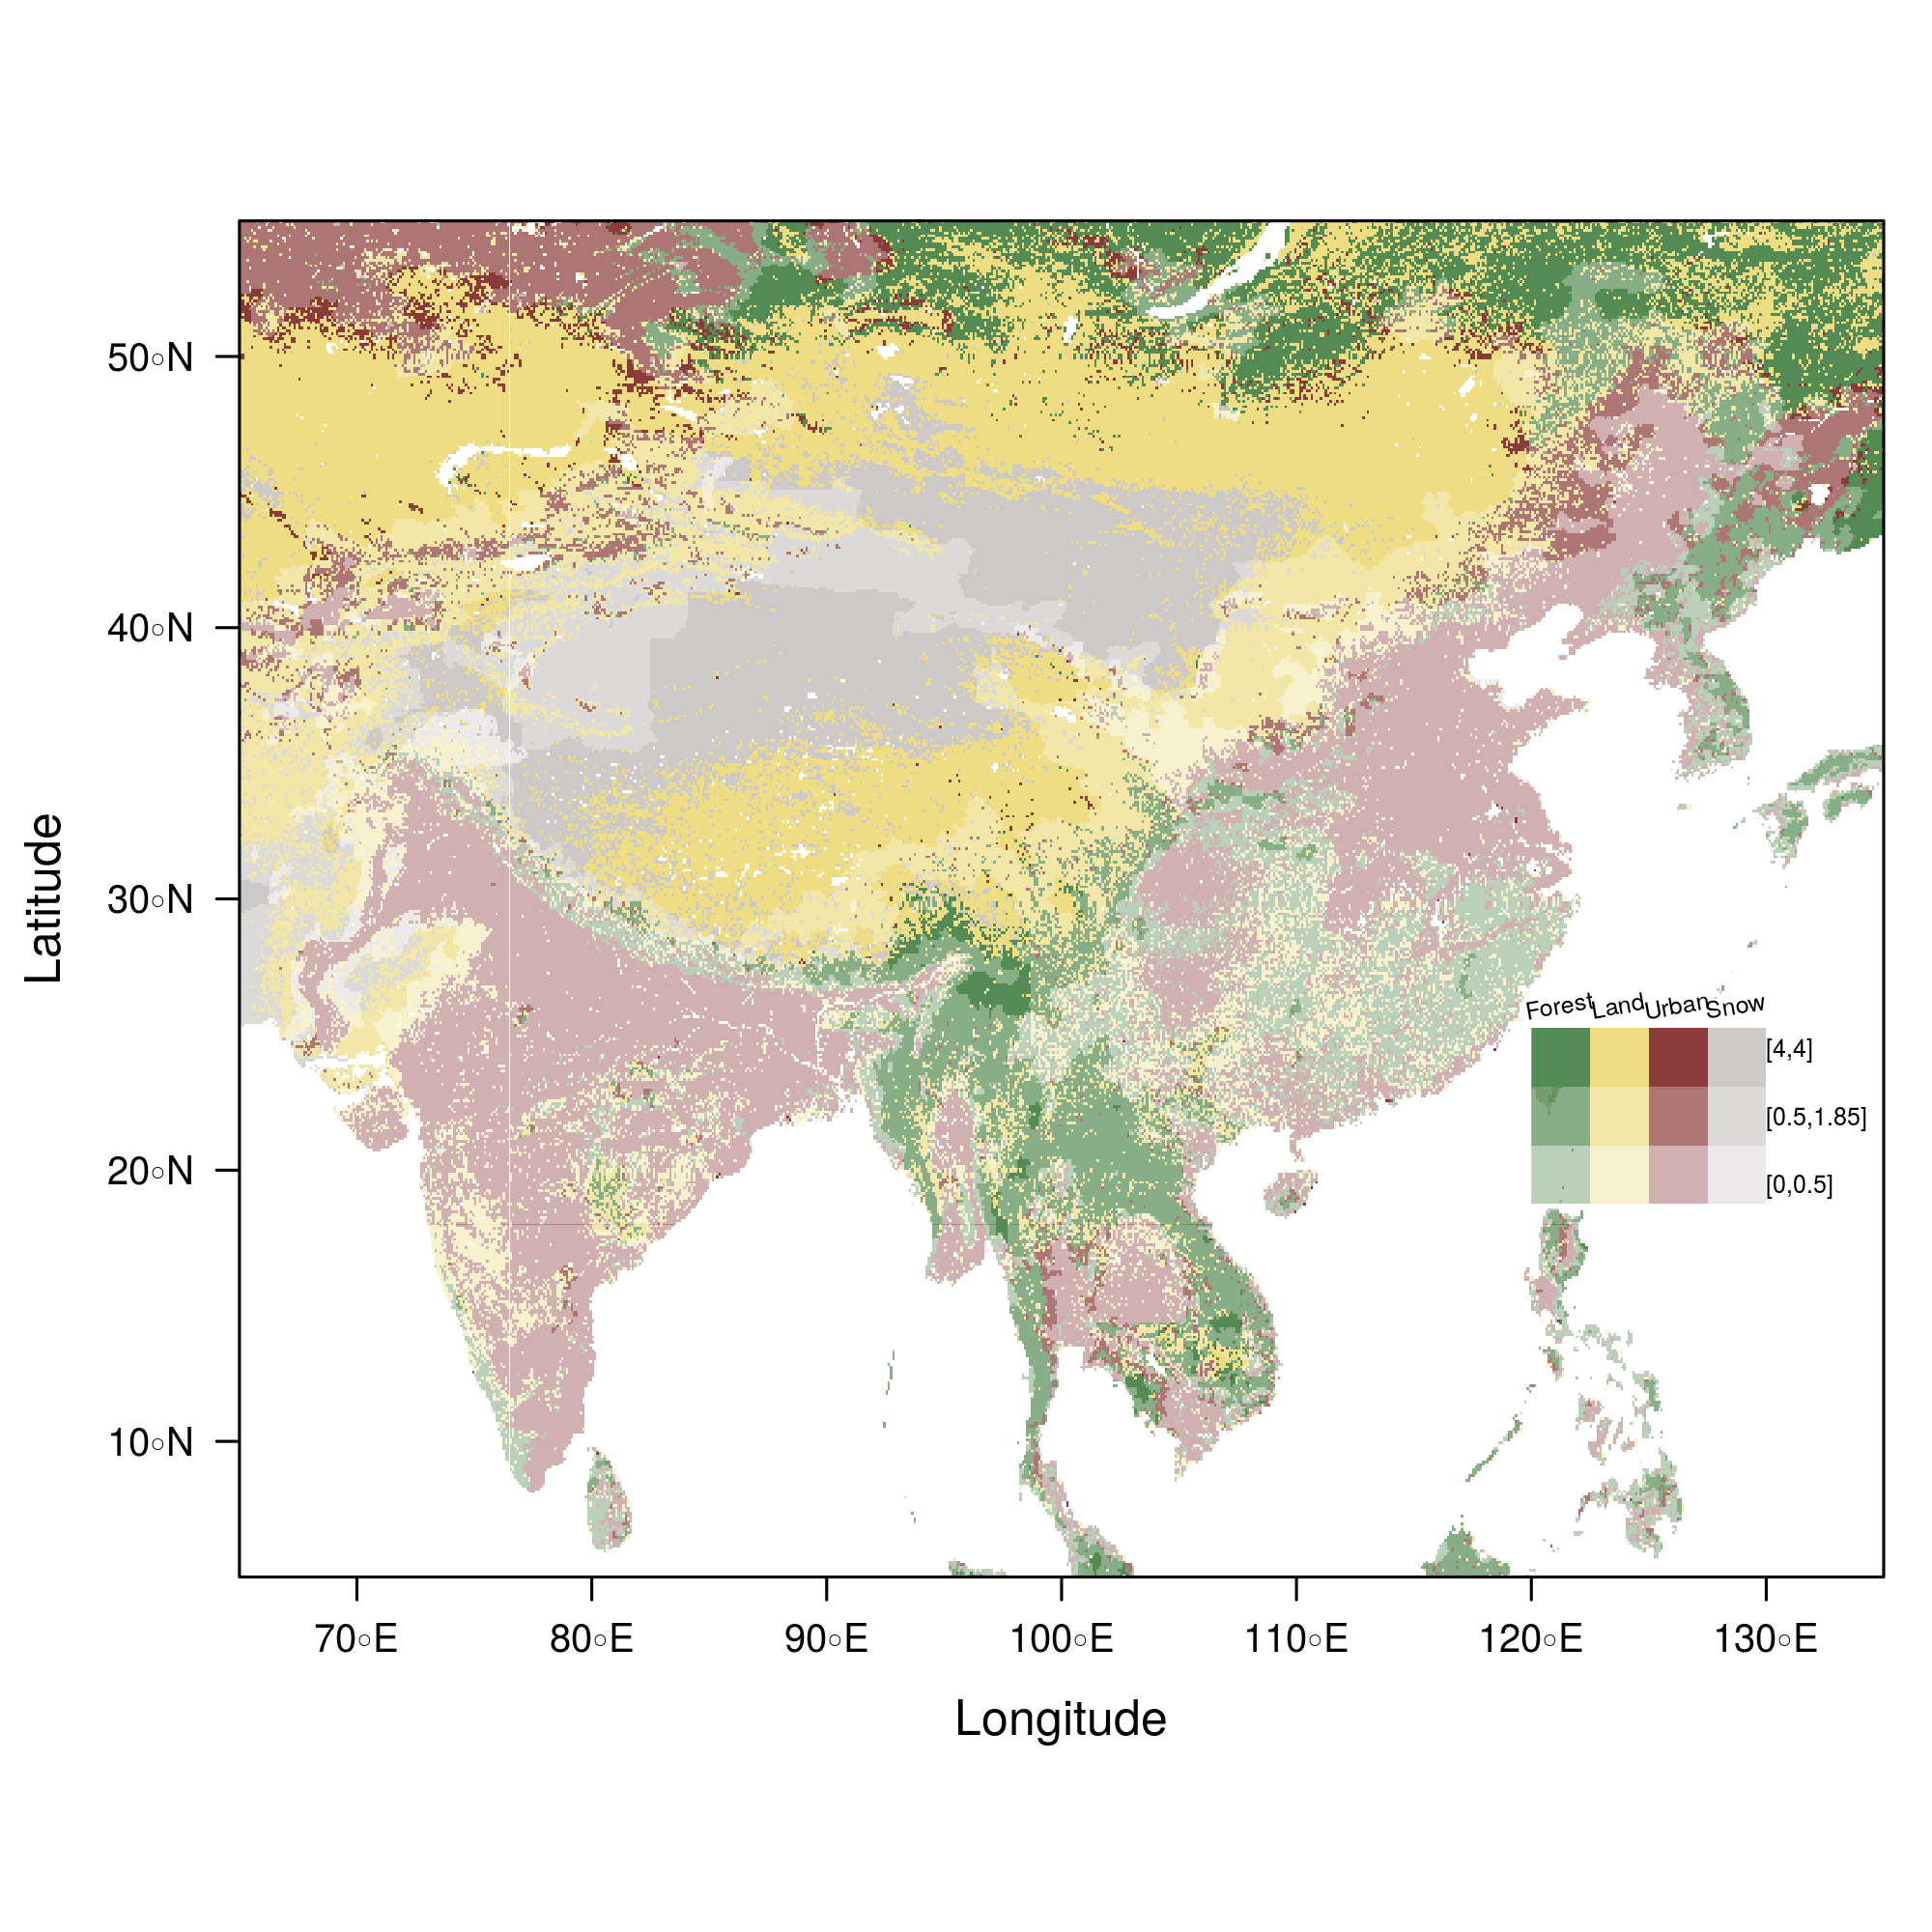
\includegraphics[width=.9\linewidth]{figs/popLandClass.png}
\caption{\label{fig:popLandClass}Population density for each land class (multivariate raster).}
\end{figure}


\section{Vector Fields}
\label{sec-1}
\label{sec:vector}

Many objects in our natural environment exhibit directional
features that are naturally represented by vector data. Vector
fields, commonly found in science and engineering, describe the
spatial distribution of a vector variable such as fluid flow or
electromagnetic forces. A suitable visualization method has to
display both the magnitude and the direction of the vectors at any
point.

This section illustrates two visualization techniques, arrow plots and
stream lines, with the help of the wind direction and speed forecast
published by MeteoGalicia (see Section \ref{sec:animationST} for
details).

\index{Packages!rasterVis@\texttt{rasterVis}}
\index{Packages!raster@\texttt{raster}}
\index{Data!Wind Speed}

\lstset{language=R,numbers=none}
\begin{lstlisting}
library(raster)
library(rasterVis)

wDir <- raster('data/wDir')/180*pi
wSpeed <- raster('data/wSpeed')
windField <- stack(wSpeed, wDir)
names(windField) <- c('magnitude', 'direction')
\end{lstlisting}

\subsection{Arrow Plot}
\label{sec-1-1}
A frequent vector visualization technique is the arrow plot, which
draws a small arrow at discrete points within the vector field
(Figure \ref{fig:vectorplot}). This approach is best suited for
small datasets. If the grid of discrete points gets too dense or
if the variations in magnitude are too big, the images tend to be
visually confusing.

\index{vectorplot@\texttt{vectorplot}}
\lstset{language=R,numbers=none}
\begin{lstlisting}
vectorplot(windField, isField=TRUE, par.settings=BTCTheme(),
	   colorkey=FALSE, scales=list(draw=FALSE))
\end{lstlisting}

\begin{figure}[htb]
\centering
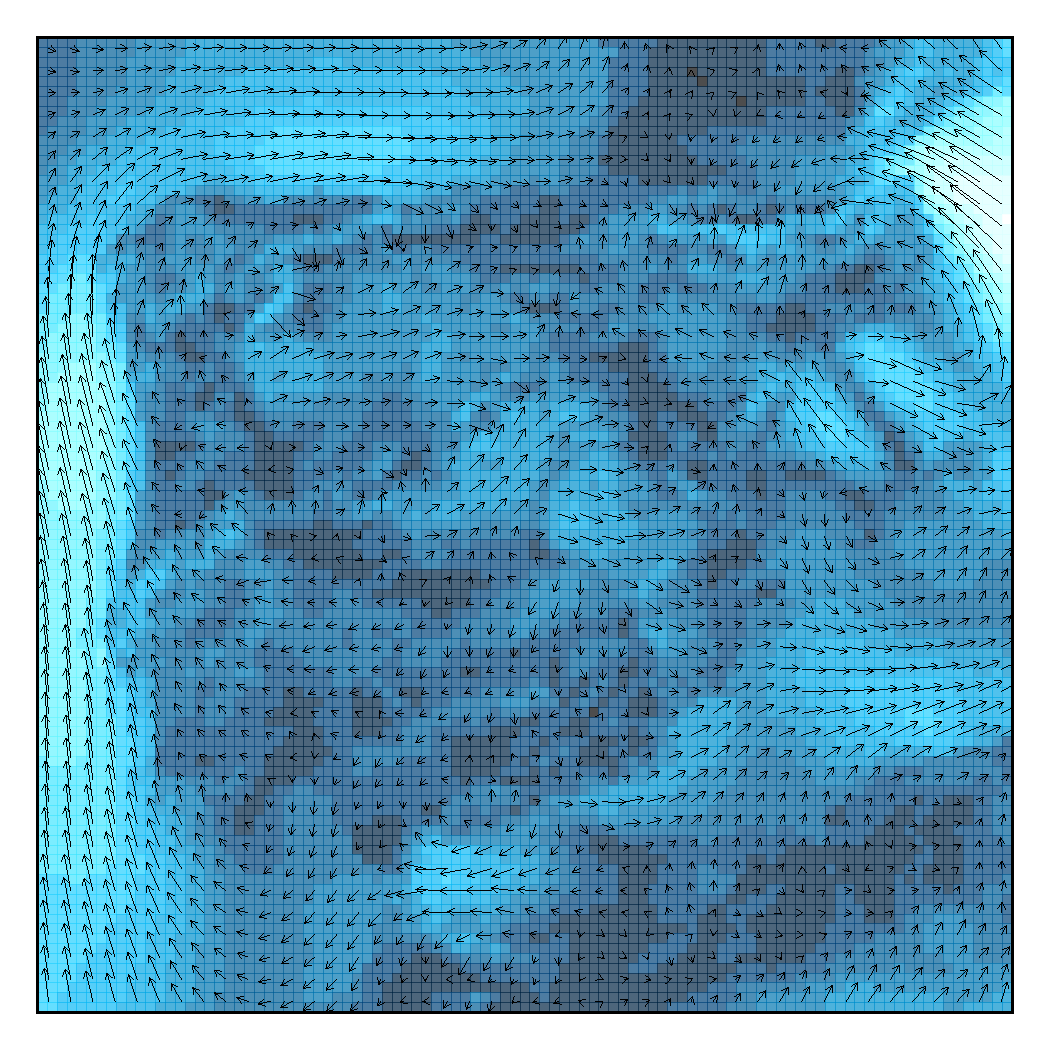
\includegraphics[width=.9\linewidth]{figs/vectorplot.pdf}
\caption{\label{fig:vectorplot}Arrow plot of the wind vector field.}
\end{figure}
\subsection{Streamlines}
\label{sec-1-2}
Another solution is to depict the directional structure of the vector
field by its integral curves, also denoted as flow lines or
streamlines. There are a variety of algorithms to produce such
visualization. The \texttt{streamplot} function of \texttt{rasterVis} displays
streamlines with a procedure inspired by the FROLIC algorithm: For
each point, \emph{droplet}, of a jittered regular grid, a short streamline
portion, \emph{streamlet}, is calculated by integrating the underlying
vector field at that point. The main color of each streamlet indicates
local vector magnitude. Streamlets are composed of points whose sizes,
positions, and color degradation encode the local vector direction
(Figure \ref{fig:streamplot}).

\index{streamplot@\texttt{streamplot}}
\index{brewer.pal@\texttt{brewer.pal}}
\lstset{language=R,numbers=none}
\begin{lstlisting}
myTheme <- streamTheme(region=rev(brewer.pal(n=4, name='Greys')),
				    symbol=BTC(n=9, beg=20))
streamplot(windField, isField=TRUE,
	   par.settings=myTheme,
	   droplet=list(pc=12),
	   streamlet=list(L=5, h=5),
	   scales=list(draw=FALSE),
	   panel=panel.levelplot.raster)
\end{lstlisting}

\begin{figure}[htb]
\centering
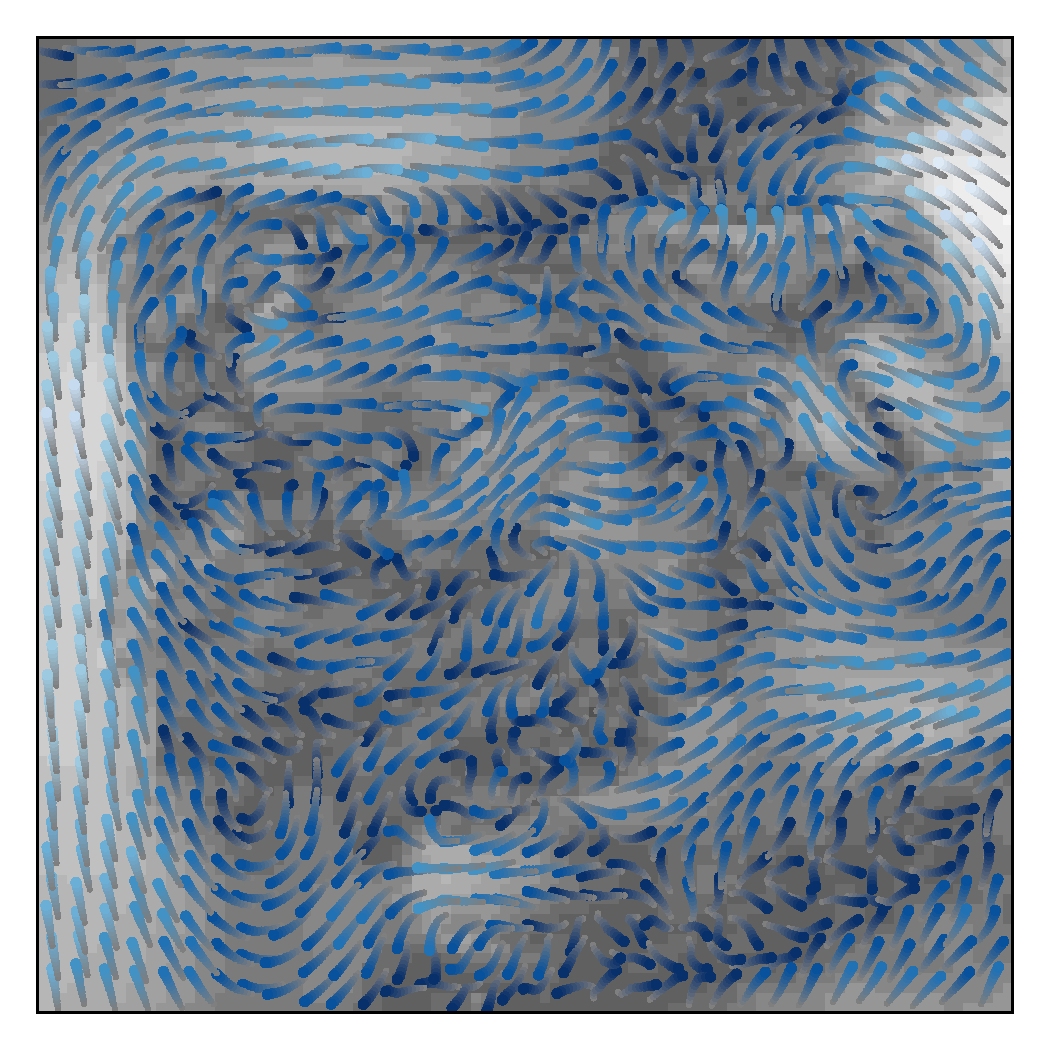
\includegraphics[width=.9\linewidth]{figs/streamplot.pdf}
\caption{\label{fig:streamplot}Streamlines of the wind vector field.}
\end{figure}

The magic of Figure \ref{fig:streamplot} is that it is able to show the
underlying physical structure of the spatial region only displaying
wind speed and direction. It is easy to recognize the Iberian
Peninsula surrounded by strong winds along the eastern and northern
coasts. Another feature easily distinguishable is the Strait of
Gibraltar, a channel that connects the Atlantic Ocean to the
Mediterranean Sea between the south of Spain and the north of
Morocco. Also apparent are the Pyrenees mountains and some of the
river valleys.


\chapter{Reference and Physical Maps}
\label{cha:refer-phys-maps}

A reference map focuses on the geographic location of features. In
these maps, cities are named and major transport routes are
identified. In addition, natural features such as rivers and mountains are
named, and elevation is shown using a simple color shading.  

A physical map shows the physical landscape features of a
place. Mountains and elevation changes are usually shown with
different colors and shades to show relief, using green to show
lower elevations and browns for high elevations.

This chapter details how to create a reference map of a northern
region of Spain using data from OpenStreetMap and a physical map of
Brazil with data from different sources.


\section{Physical Maps}
\label{sec-1}
Brazil\footnote{\url{http://en.wikipedia.org/wiki/Brazil}}, the world's fifth largest country, is one of the
seventeen megadiverse countries\footnote{\url{http://en.wikipedia.org/wiki/Megadiverse_countries}}, home to diverse wildlife,
natural environments, and extensive natural resources in a variety of
protected habitats. Throughout this section we will create a physical
map of this exceptional country using data from several data services.

\index{Packages!raster@\texttt{raster}}  
\index{Packages!rasterVis@\texttt{rasterVis}}  
\index{Packages!sp@\texttt{sp}}  
\index{Packages!maptools@\texttt{maptools}}  
\index{Packages!rgeos@\texttt{rgeos}}  
\index{Packages!colorspace@\texttt{colorspace}}  
\index{CRS@\texttt{CRS}}

\lstset{language=R,numbers=none}
\begin{lstlisting}
library(raster)
library(rasterVis)
library(maptools)
library(rgeos)
library(latticeExtra)
library(colorspace)

## Longitude-Latitude projection
proj <- CRS(' +proj=longlat +ellps=WGS84')
\end{lstlisting}

\subsection{Retrieving Data}
\label{sec-1-1}
Four types of information are needed: administrative boundaries,
terrain elevation, rivers and lakes, and sea depth.

\index{download.file@\texttt{download.file}}
\index{readShapePoly@\texttt{readShapePoly}}
\index{readShapeLines@\texttt{readShapeLines}}
\index{Encoding@\texttt{Encoding}}
\index{raster@\texttt{raster}}
\index{Data!GADM}
\index{Data!DIVA-GIS}
\index{Data!Natural Earth Data}

\begin{enumerate}
\item The administrative boundaries are available from GADM\footnote{\url{http://gadm.org/}}. The
\texttt{readShapePoly} function reads data from the downloaded shapefile
and creates a \texttt{SpatialPolygonsDataFrame} object.
\lstset{language=R,numbers=none}
\begin{lstlisting}
old <- setwd(tempdir())

download.file('http://www.gadm.org/data/shp/BRA_adm.zip',
	      'BRA_adm.zip')
unzip('BRA_adm.zip')
brazilAdm <- readShapePoly('BRA_adm1.shp', proj4string=proj)
Encoding(levels(brazilAdm$NAME_1)) <- 'latin1'
\end{lstlisting}

\item The terrain elevation or digital elevation model (DEM) is
available from DIVA-GIS\footnote{\url{http://www.diva-gis.org/Data}}. The \texttt{raster} function reads the
file and creates a \texttt{RasterLayer} object.
\lstset{language=R,numbers=none}
\begin{lstlisting}
download.file('http://www.diva-gis.org/data/alt/BRA_alt.zip',
	      'BRA_alt.zip')
unzip('BRA_alt.zip')
brazilDEM <- raster('BRA_alt')
\end{lstlisting}
\item The water lines (rivers and lakes) are available from Natural
Earth Data\footnote{\url{http://www.naturalearthdata.com/}}. The \texttt{readShapeLines} function reads data from
the downloaded shapefile and creates a \texttt{SpatialLinesDataFrame}
object.
\lstset{language=R,numbers=none}
\begin{lstlisting}
## World Water lines (Natural Earth)
download.file('http://www.naturalearthdata.com/http//www.naturalearthdata.com/download/10m/physical/ne_10m_rivers_lake_centerlines.zip',
	      'neRivers.zip')
unzip('neRivers.zip')
worldlRiv <- readShapeLines('ne_10m_rivers_lake_centerlines', proj4string = proj)
\end{lstlisting}
\item Finally, the sea depth is also available from Natural Earth
Data\footnotemark[5]{}. The raster covers the whole world so it must be
cropped by the extent of the DEM raster.
\lstset{language=R,numbers=none}
\begin{lstlisting}
download.file('http://www.naturalearthdata.com/http//www.naturalearthdata.com/download/10m/raster/OB_LR.zip',
	      'neSea.zip')
unzip('neSea.zip')
worldSea <- raster('OB_LR.tif')
brazilSea <- crop(worldSea, brazilDEM)
setwd(old)
\end{lstlisting}
\end{enumerate}
\subsection{Intersection of Shapefiles and Elevation Model}
\label{sec-1-2}
The rivers and lakes database from Natural Earth Data comprises all
the world extent, but we only need the rivers of Brazil. The function
\texttt{gIntersection} of the package \texttt{rgeos} determines the intersection
between two geometries. Because these geometries must be defined with
classes of the \texttt{sp} package, the extent of \texttt{brazilDEM} must be first
converted to \texttt{SpatialPolygons}. The intersection is a new
\texttt{SpatialLines} object, \texttt{brazilRiv}.

\index{gIntersection@\texttt{gIntersection}}
\index{extent@\texttt{extent}}

\lstset{language=R,numbers=none}
\begin{lstlisting}
## only those features labeled as "River" are needed
worlRiv<- worlRiv[worlRiv$featurecla=='River',]

## Define the extent of Brazil as a SpatialPolygons
extBrazil <- as(extent(brazilDEM), 'SpatialPolygons')
proj4string(extBrazil) <- proj

## and intersect it with worldRiv to extract brazilian rivers
## from the world database
brazilRiv <- gIntersection(worldRiv, extBrazil, byid=TRUE)
## and especially the famous Amazonas River
amazonas <- worldRiv[worldRiv$name=='Amazonas',]
\end{lstlisting}
\subsection{Labels}
\label{sec-1-3}
Each region of Brazil will be labeled with the name of its
corresponding polygon. The locations of the labels are defined by the
centroid of each polygon, easily computed with the \texttt{coordinates}
method. In addition, a larger label with the name of the country will be
placed in the average centroid.

\index{coordinates@\texttt{coordinates}}
\index{apply@\texttt{apply}}

\lstset{language=R,numbers=none}
\begin{lstlisting}
## Locations of labels of each polygon
centroids <- coordinates(brazilAdm)
## Location of the "Brazil" label (average of the set of polygons centroids)
xyBrazil <- apply(centroids, 2, mean)
\end{lstlisting}

Some region names are too long to be displayed in one line. Thus, a
previous step is to split the string if it comprises more than two
words.

\index{sapply@\texttt{sapply}}
\index{strsplit@\texttt{strsplit}}

\lstset{language=R,numbers=none}
\begin{lstlisting}
admNames <- strsplit(as.character(brazilAdm$NAME_1), ' ')

admNames <- sapply(admNames,
		 FUN=function(s){
		   sep=if (length(s)>2) '\n' else  ' '
		   paste(s, collapse=sep)
		   })
\end{lstlisting}
\subsection{Overlaying Layers of Information}
\label{sec-1-4}
Therefore, the physical map (Figure \ref{fig:brazil}) is composed
of four layers: 

\begin{enumerate}
\item The sea depth raster displayed with the \texttt{levelplot} method of the
\texttt{rasterVis} package. The palette is defined with \texttt{brewer.pal}
(Figure \ref{fig:rastersBrazil}).
\lstset{language=R,numbers=none}
\begin{lstlisting}
blueTheme <- rasterTheme(region=brewer.pal(n=9, 'Blues'))

seaPlot <- levelplot(brazilSea, par.settings=blueTheme,
		    maxpixels=1e6, panel=panel.levelplot.raster,
		    margin=FALSE, colorkey=FALSE)
\end{lstlisting}

\index{rasterTheme@\texttt{rasterTheme}}
\index{brewer.pal@\texttt{brewer.pal}}

\item The altitude raster layer uses a terrain colors palette, as the one
produced by the \texttt{terrain\_hcl} function from the \texttt{colorspace} package
\cite{Ihaka.Murrell.ea2011} (Figure \ref{fig:rastersBrazil}).
\lstset{language=R,numbers=none}
\begin{lstlisting}
terrainTheme <- rasterTheme(region=terrain_hcl(15))

altPlot <- levelplot(brazilDEM, par.settings=terrainTheme,
		     maxpixels=1e6, panel=panel.levelplot.raster,
		     margin=FALSE, colorkey=FALSE)
\end{lstlisting}

\index{rasterTheme@\texttt{rasterTheme}}
\index{terrain_hcl@\texttt{terrain\_hcl}}

\item The rivers represented by the \texttt{SpatialLinesDataFrame} object. The
Amazonas River is labeled with \texttt{sp.lineLabel} and printed with a
thicker line. The label is created with the \texttt{label} method, a
wrapper function to extract the \texttt{ID} slots from the \texttt{SpatialLines}
and create a suitable \texttt{character} object with the correct \texttt{names}
values.

\lstset{language=R,numbers=none}
\begin{lstlisting}
amazonasLab <- label(amazonas, 'Amazonas')
\end{lstlisting}

\item The administrative boundaries represented by the
\texttt{SpatialPolygonsDataFrame} object with their labels printed with
the \texttt{panel.pointLabel} function. This function uses optimization
routines to find good locations for point labels without overlaps.

\index{levelplot@\texttt{levelplot}}
\index{sp.lines@\texttt{sp.lines}}
\index{sp.lineLabel@\texttt{sp.lineLabel}}
\index{sp.polygons@\texttt{sp.polygons}}
\index{panel.text@\texttt{panel.text}}
\index{layer@\texttt{layer}}
\index{brewer.pal@\texttt{brewer.pal}}

\lstset{language=R,numbers=none}
\begin{lstlisting}
 seaPlot + altPlot + layer({
    ## Rivers
    sp.lines(brazilRiv, col='darkblue', lwd=0.2)
    ## Amazonas
    sp.lineLabel(amazonas, amazonasLab, 
		 lwd=1, col='darkblue', col.line='darkblue',
		 cex=0.5, fontfamily='Palatino')
    ## Administrative boundaries
    sp.polygons(brazilAdm, col='black', lwd=0.2)
    ## Centroids of administrative boundaries ...
    panel.points(centroids, col='black')
    ## ... with their labels
    panel.pointLabel(centroids, labels=admNames,
		     cex=0.7, fontfamily='Palatino', lineheight=.8)
    ## Country name
    panel.text(xyBrazil[1], xyBrazil[2], labels='B R A Z I L',
	       cex=1.5, fontfamily = 'Palatino', fontface=2)
})
\end{lstlisting}
\end{enumerate}

\begin{figure}[htb]
\centering
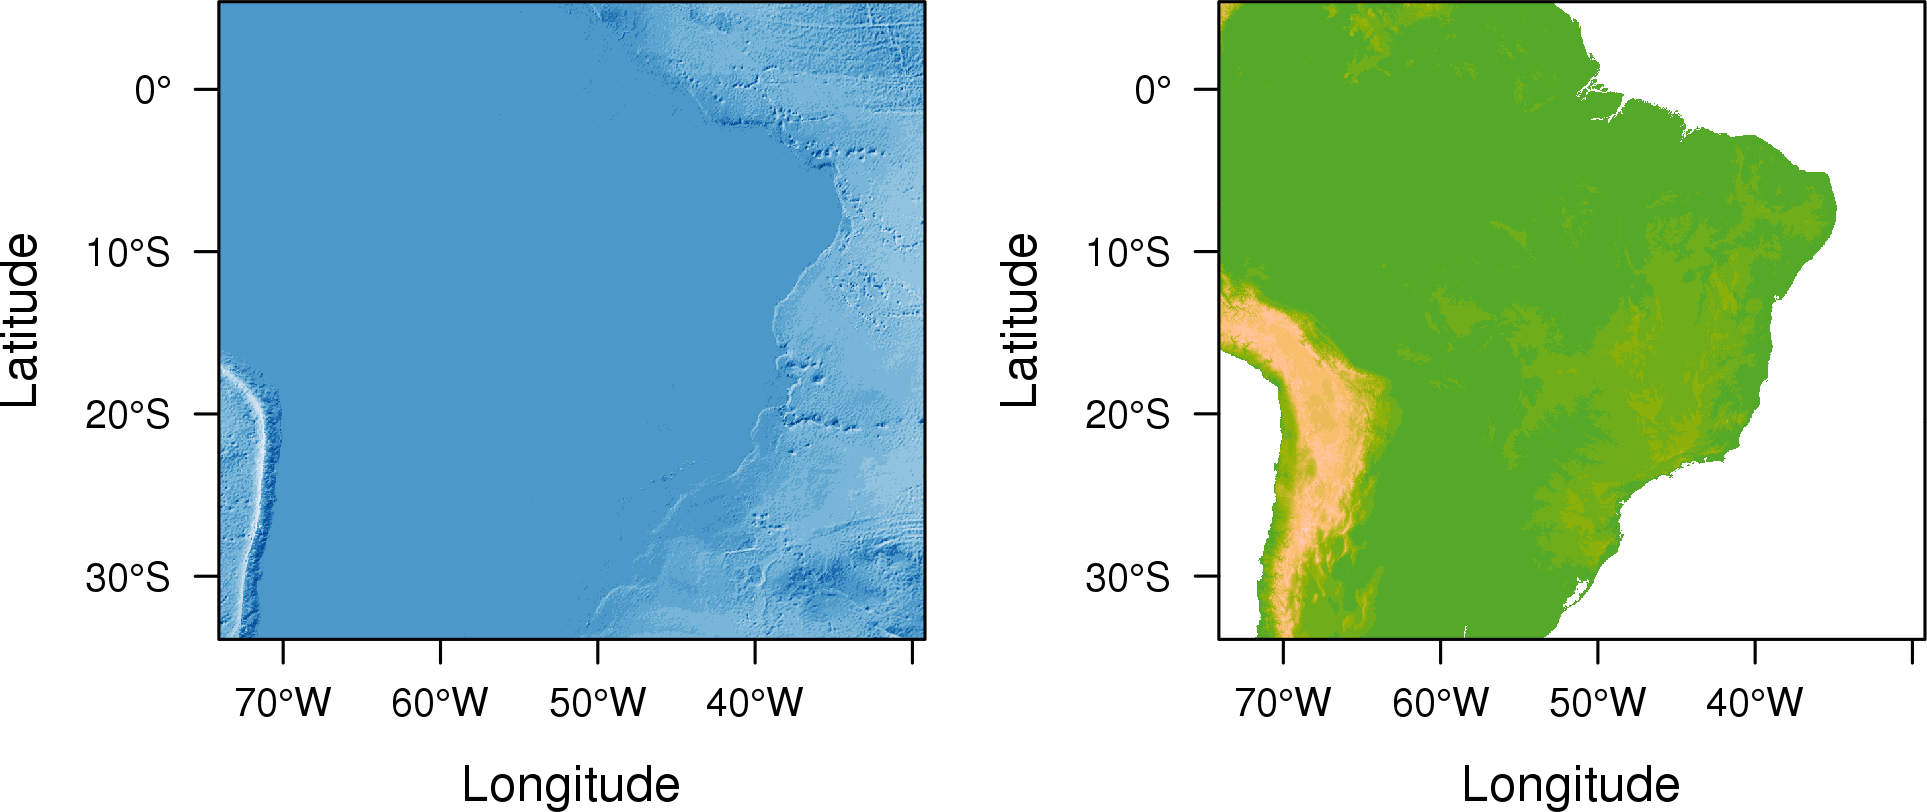
\includegraphics[width=.9\linewidth]{figs/rastersBrazil.png}
\caption{\label{fig:rastersBrazil}Sea depth and altitude rasters of Brazil.}
\end{figure}


\begin{figure}[htb]
\centering
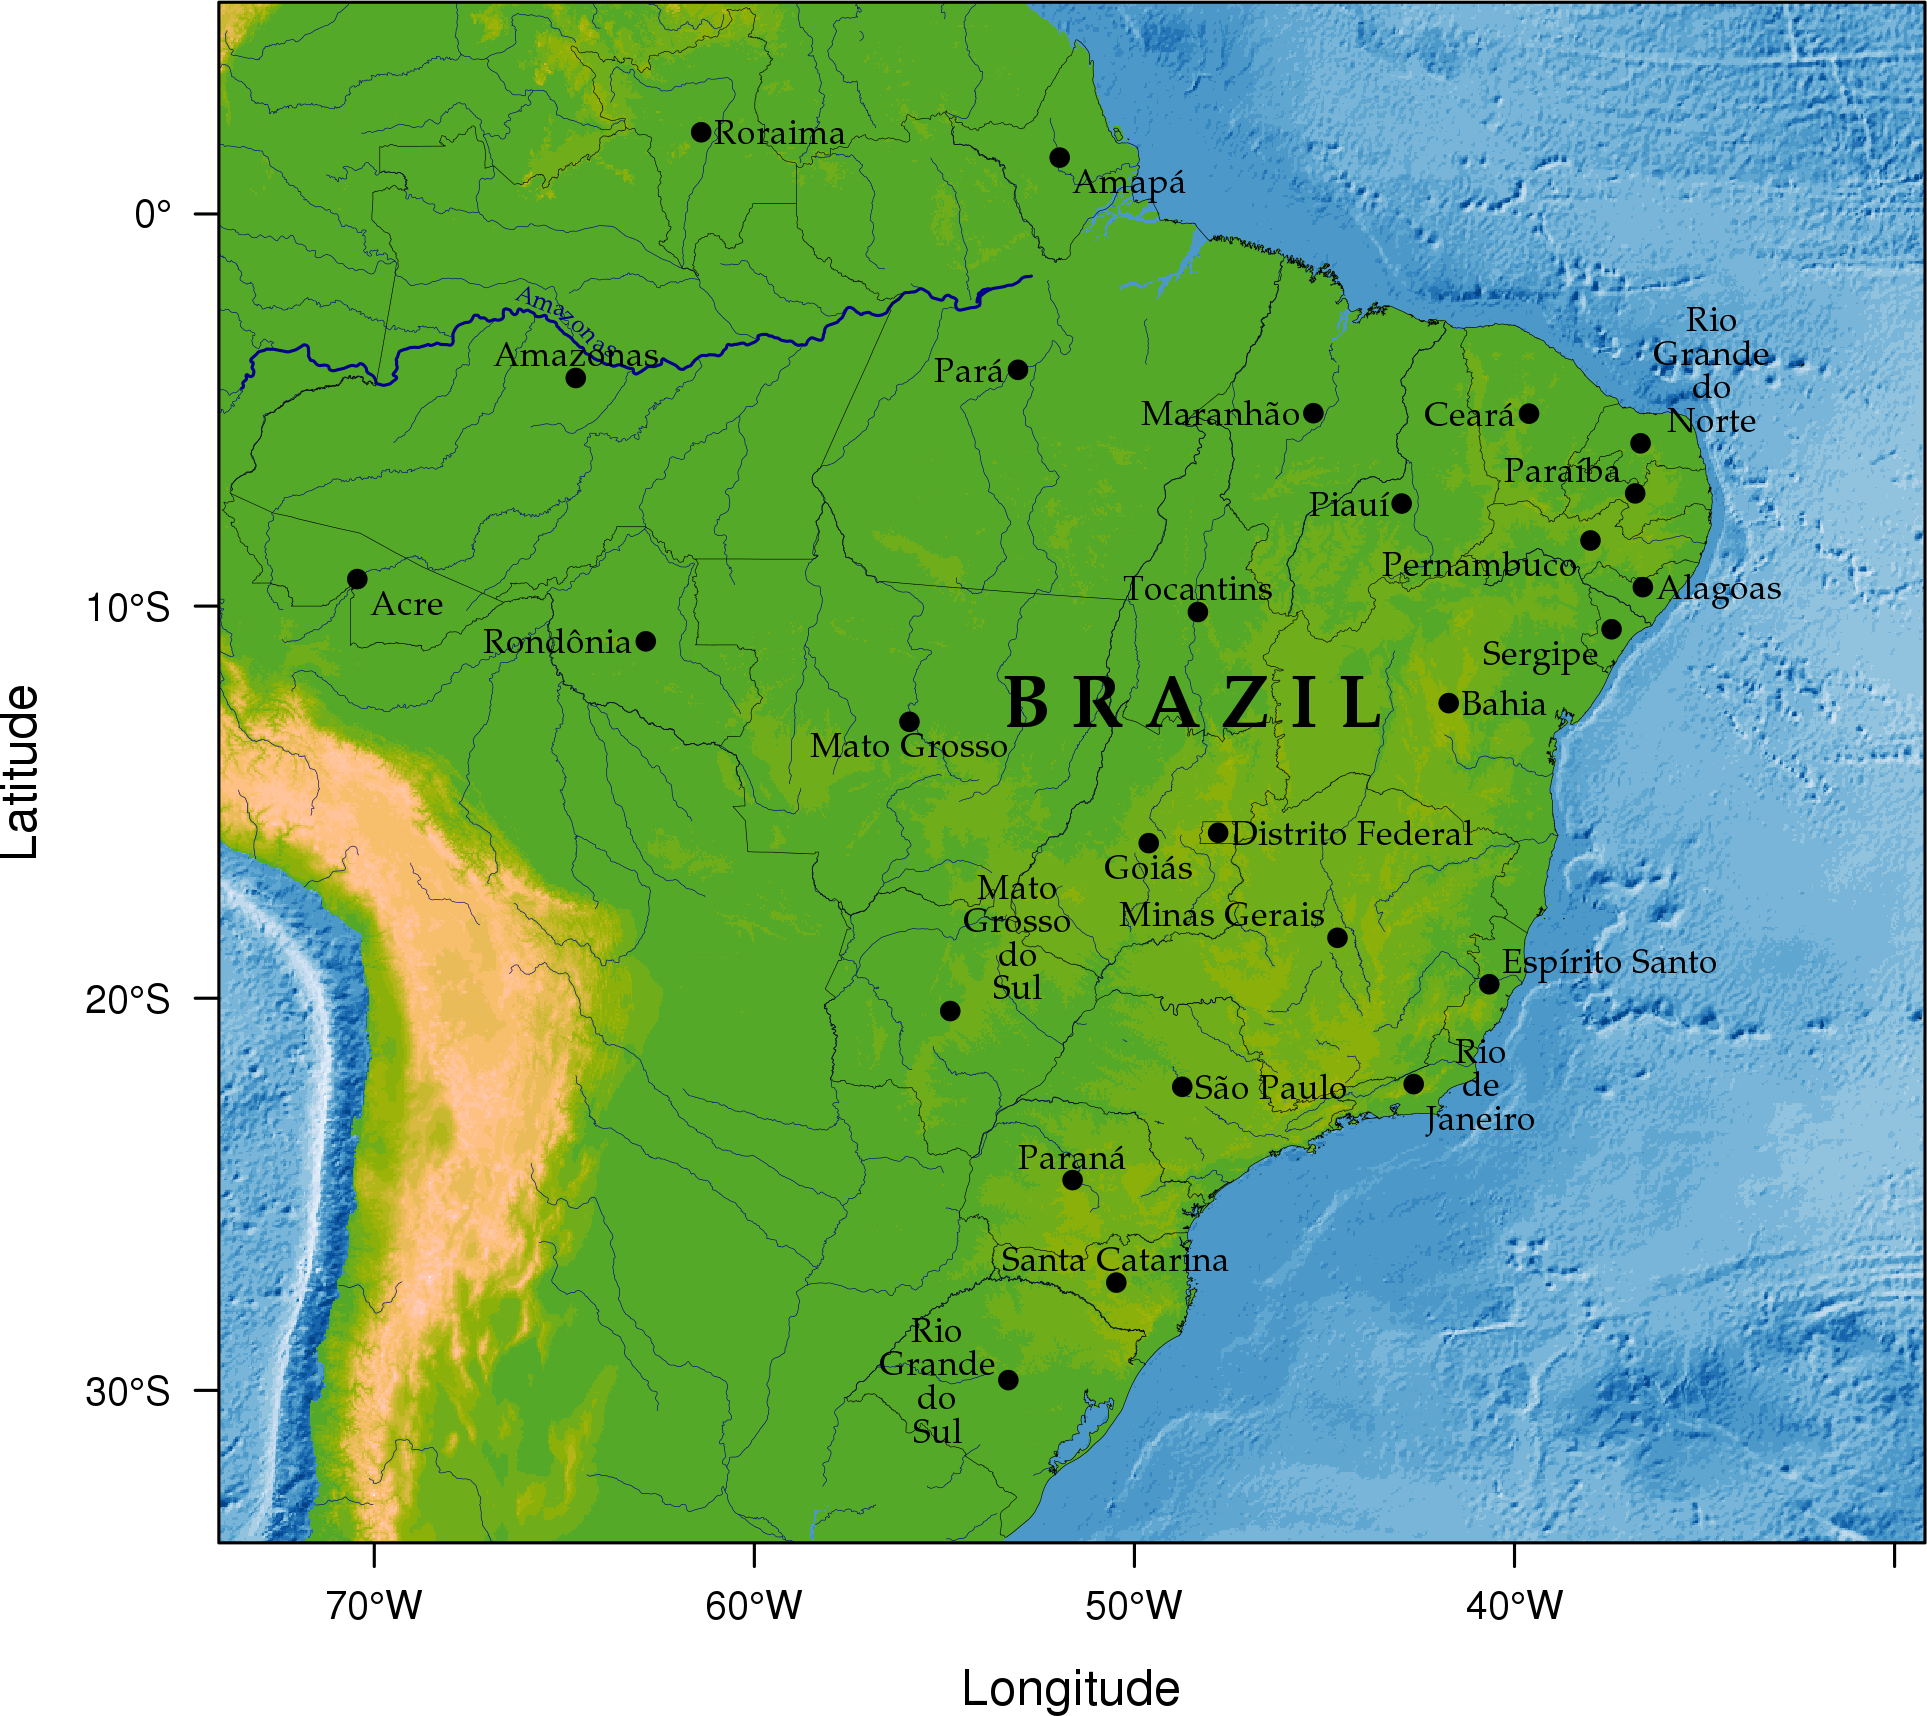
\includegraphics[width=.9\linewidth]{figs/brazil.png}
\caption{\label{fig:brazil}Physical map of Brazil. Main administrative regions and the Amazonas River are labeled.}
\end{figure}


\section{\floweroneleft OpenStreetMap with Hill Shade Layers}
\label{sec-1}

Although I was born in Madrid, Galicia (north of Spain) is a very
special region for me. More precisely, the Cedeira and Valdoviño
regions offer a wonderful combination of wild sea, secluded beaches,
and forests. I will show you a map of these marvelous places.

\subsection{Retrieving Data from OpenStreetMap}
\label{sec-1-1}
The first step is to acquire information from the OpenStreetMap
project. There are several packages to extract data from this service
but, while most of them only provide already rendered raster images,
the \texttt{osmar} package\footnote{Its webpage \url{http://osmar.r-forge.r-project.org/} proposes
two interesting demos.} \cite{Eugster.Schlesinger2010} enables the
use of the raw data with classes from the packages \texttt{sp} and \texttt{igraph}.

The \texttt{get\_osm} function retrieves a region defined by \texttt{corner\_bbox}
using the OSM API.

\index{Data!OpenStreetMap}
\index{Packages!osmar@\texttt{osmar}}
\index{osmsource_api@\texttt{osmsource\_api}}
\index{get_osm@\texttt{get\_osm}}

\lstset{language=R,numbers=none}
\begin{lstlisting}
library('osmar')

api <- osmsource_api()
ymax <- 43.7031
ymin <- 43.6181
xmax <- -8.0224
xmin <- -8.0808
box <- corner_bbox(xmin, ymin, xmax, ymax)
cedeira <- get_osm(box, source=api, full=TRUE)
\end{lstlisting}

The \texttt{cedeira} object includes three main components: nodes, ways and
relations. These components can be accessed with the functions \texttt{find},
\texttt{subset}, \texttt{way}, \texttt{node}, \texttt{relation}, and \texttt{tags}. Thus, the different
kinds of roads can be obtained using \texttt{way} and \texttt{tags} with the
appropiate tag.

\lstset{language=R,numbers=none}
\begin{lstlisting}
summary(cedeira$nodes)
\end{lstlisting}

\index{find@\texttt{find}}
\index{subset@\texttt{subset}}
\index{way@\texttt{way}}

\lstset{language=R,numbers=none}
\begin{lstlisting}
idxHighways <- find(cedeira, way(tags(k=='highway')))
highways <- subset(cedeira, way_ids=idxHighways)
idxStreets <- find(highways, way(tags(v=='residential')))
idxPrimary <- find(highways, way(tags(v=='primary')))
idxSecondary <- find(highways, way(tags(v=='secondary')))
idxTertiary <- find(highways, way(tags(v=='tertiary')))
idxOther <- find(highways,
		 way(tags(v=='unclassified' |
			  v=='footway' |
			  v=='steps')))
\end{lstlisting}

The result of \texttt{find} is the index of each element. The correspondent
spatial object is extracted with \texttt{find\_down} and \texttt{subset}, and can be
converted to a class defined by the \texttt{sp} package with \texttt{as\_sp}. The
following \texttt{spFromOSM} function encodes the procedure, and extracts the
\texttt{SpatialLines} object that represent each type of road.

\index{as_sp@\texttt{as\_sp}}
\index{find_down@\texttt{find\_down}}

\lstset{language=R,numbers=none}
\begin{lstlisting}
spFromOSM <- function(source, index, type='lines'){
  idx <- find_down(source, index)
  obj <- subset(source, ids=idx)
  objSP <- as_sp(obj, type)
  }

streets <- spFromOSM(cedeira, way(idxStreets))
primary <- spFromOSM(cedeira, way(idxPrimary))
secondary <- spFromOSM(cedeira, way(idxSecondary))
tertiary <- spFromOSM(cedeira, way(idxTertiary))
other <- spFromOSM(cedeira, way(idxOther))
\end{lstlisting}

A similar procedure can be applied to construct a \texttt{SpatialPoints}
object with the collection of places with name:

\index{match@\texttt{match}}

\lstset{language=R,numbers=none}
\begin{lstlisting}
idxPlaces <- find(cedeira, node(tags(k=='name')))
places <- spFromOSM(cedeira, node(idxPlaces), 'points')

nms <- subset(cedeira$nodes$tags, subset=(k=='name'), select=c('id', 'v'))
ord <- match(idxPlaces, nms$id)
nms <- nms[ord,]
places$name <- nms$v[ord]

## Cedeira town will be printed differently
idxCedeira <- which(nms$v=='Cedeira') ##Main town
cedeiraCoords <- coordinates(places[idxCedeira,])
places <- places[-idxCedeira,]
\end{lstlisting}
\subsection{Hill Shading}
\label{sec-1-2}
\index{Hill shading}

The second step is to produce layers to display the topography. A
suitable method is shaded relief or hill shading. This technique
simulates the cast shadow thrown from a light source upon a raised
relief map. The hill shade layer can be computed from the slope and
aspect layers derived from a Digital Elevation Model (DEM). This layer
will underlay the DEM raster, which will be printed using
semitransparency.

The DEM for this region is available at the Geonetwork-SECAD service
from the Universidad de Extremadura and can be read with \texttt{raster}:

\index{Packages!raster@\texttt{raster}}
\index{Packages!rasterVis@\texttt{rasterVis}}
\index{Data!Geonetwork}

\lstset{language=R,numbers=none}
\begin{lstlisting}
library(raster)
## Galicia DEM
## http://ide.unex.es/geonetwork/srv/es/main.search?any=MDE_Galicia
## http://ide.unex.es:8180/geonetwork/srv/es/resources.get?id=21&fname=dem_gal.7z&access=private

old <- tempdir()
download.file('http://ide.unex.es:8180/geonetwork/srv/es/resources.get?id=21&fname=dem_gal.7z&access=private', 'dem_gal.7z')
unzip('dem_gal.7z')
demGalicia <- raster('dem_gal.asc')
setwd(old)
\end{lstlisting}

The \texttt{slope} and \texttt{aspect} layers are computed with the \texttt{terrain}
function, and the hill shade layer is derived with these layers for a
fixed sun position. Previously, the useful region of the DEM raster
was extracted with the \texttt{crop} function:

\index{terrain@\texttt{terrain}}
\index{crop@\texttt{crop}}
\index{hillShade@\texttt{hillShade}}
\index{Hill shading}

\lstset{language=R,numbers=none}
\begin{lstlisting}
cedeiraSP <- as_sp(cedeira, 'points')
projCedeira <- projection(cedeiraSP)
##extCedeira <- bbox(cedeiraSP) 
## or summary(cedeira$nodes)$bbox
extCedeira <- extent(-8.15, -7.95, 43.6, 43.75)
demCedeira <- crop(demGalicia, extCedeira)
projection(demCedeira) <- projCedeira
demCedeira[demCedeira <= 0] <- NA

slope <- terrain(demCedeira, 'slope')
aspect <- terrain(demCedeira, 'aspect')
hsCedeira <- hillShade(slope=slope, aspect=aspect,
		       angle=20, direction=30)
\end{lstlisting}
\subsection{Overlaying Layers of Information}
\label{sec-1-3}
And finally, the third step is to display the different layers of
information in correct order (Figure \ref{fig:cedeiraOsmar}):

\begin{itemize}
\item The hill shade layer is created with the \texttt{levelplot} method for
  \texttt{Raster} objects defined in the \texttt{rasterVis} package. The
  \texttt{GrTheme} is modified to display the sea region with blue color.

\item The DEM raster is printed with terrain colors and
semitransparency over the hill shade layer.

\item The roads are displayed with an auxiliary function (\texttt{sp.road})
that produces a colored line over a thicker black line.

\item The places are represented with \texttt{sp.points} and labeled with
the \texttt{sp.pointLabel} method, a modification of the \texttt{pointLabel}
function for \texttt{base} graphics, both defined in the \texttt{maptools}
package. These functions use optimization routines to find good
locations for point labels without overlaps.
\end{itemize}

\index{Packages!maptools@\texttt{maptools}}  
\index{Packages!sp@\texttt{sp}}  
\index{Packages!latticeExtra@\texttt{latticeExtra}}  
\index{Packages!colorspace@\texttt{colorspace}}  
\index{sp.lines@\texttt{sp.lines}}
\index{sp.lines@\texttt{sp.points}}
\index{sp.lines@\texttt{sp.pointLabel}}

\lstset{language=R,numbers=none}
\begin{lstlisting}
library(maptools)
library(latticeExtra)
library(colorspace)
library(rasterVis)

##Auxiliary function to display the roads. A thicker black line in
##the background and a thinner one with an appropiate color.
sp.road <- function(line, lwd=5, blwd=7,
		    col='indianred1', bcol='black'){
  sp.lines(line, lwd=blwd, col=bcol)
  sp.lines(line, lwd=lwd, col=col)
}

## The background color of the panel is set to blue to represent the sea
hsTheme <- modifyList(GrTheme(), list(panel.background=list(col='skyblue3')))
## DEM with terrain colors and semitransparency
terrainTheme <- modifyList(rasterTheme(region=terrain_hcl(n=15)),
				list(regions=list(alpha=0.6)))
## Hill shade and DEM overlaid
levelplot(hsCedeira, maxpixels=ncell(hsCedeira),
	  par.settings=hsTheme, margin=FALSE, colorkey=FALSE) +
  levelplot(demCedeira, maxpixels=ncell(demCedeira),
	    par.settings=terrainTheme) +
  ## Roads and places
  layer({
    ## Street and roads
    sp.road(streets, lwd=1, blwd=2, col='white')
    sp.road(other, lwd=2, blwd=3, col='white')
    sp.road(tertiary, lwd=3, blwd=4, col='palegreen')
    sp.road(secondary, lwd=4, blwd=6, col='midnightblue')
    sp.road(primary, col='indianred1')
    ## Places except Cedeira town
    sp.points(places, pch=19, col='black', cex=0.4, alpha=0.8)
    sp.pointLabel(places, labels=places$name,
		      fontfamily = 'Palatino', 
		      cex=0.6, col='black')
    ## Cedeira town
    panel.points(cedeiraCoords, pch=18, col='black', cex=1)
    panel.text(cedeiraCoords, labels='Cedeira', pos=2, offset=1)
    })
\end{lstlisting}

\begin{figure}[htb]
\centering
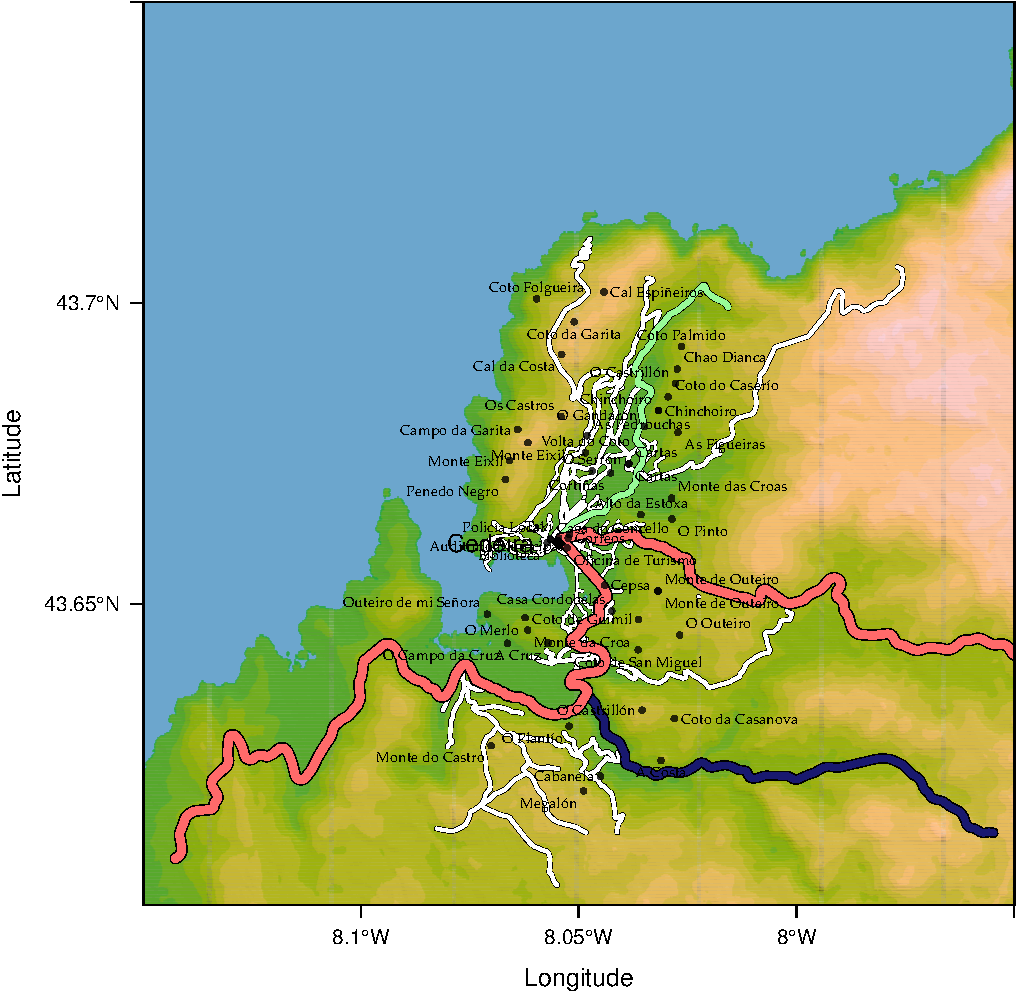
\includegraphics[width=.9\linewidth]{figs/cedeiraOsmar.pdf}
\caption{\label{fig:cedeiraOsmar}Main roads near Cedeira, Galicia. Local topography is displayed with the hill shading technique. Some places are highlighted.}
\end{figure}


\chapter{About the Data}
\label{cha:dataSpatial}


\section{Air Quality in Madrid}
\label{sec-1}
\label{sec:airQualityData}

Air pollution is harmful to health and contributes to respiratory and
cardiac diseases, and has a negative impact on natural ecosystems,
agriculture, and the built environment. In Spain, the principal
pollutants are particulate matter (PM), tropospheric ozone, nitrogen
dioxide, and environmental noise\footnote{\url{http://www.eea.europa.eu/soer/countries/es/}}.

The surveillance system of the Integrated Air Quality system of the
Madrid City Council consists of twenty-four remote stations, equipped
with analyzers for gases (NO\_\{X\}, CO, ozone, BT\_\{X\}, HCs, SO\_\{2\}) and
particles (PM10, PM2.5), which measure pollution in different areas of
the urban environment. In addition, many of the stations also include
sensors to provide meteorological data.

The detailed information of each measuring station can be retrieved
from its own webpage defined by its station code.
\lstset{language=R,numbers=none}
\begin{lstlisting}
## codeStations.csv is extracted from the document
## http://www.mambiente.munimadrid.es/opencms/export/sites/default/calaire/Anexos/INTPHORA-DIA.pdf,
## table of page 3.

codEstaciones <- read.csv2('data/codeStations.csv')
codURL <- as.numeric(substr(codEstaciones$Codigo, 7, 8))

## The information of each measuring station is available at its own webpage, defined by codURL
URLs <- paste('http://www.mambiente.munimadrid.es/opencms/opencms/calaire/contenidos/estaciones/estacion', codURL, '.html', sep='')
\end{lstlisting}

\subsection{\floweroneleft Data Arrangement}
\label{sec-1-1}
The station webpage includes several tables that can be extracted with
the \texttt{readHTMLTable} function of the \texttt{XML} package.  The longitude and
latitude are included in the second table. The \texttt{ub2dms} function
cleans this table and converts the strings to the \texttt{DMS} class defined
by the \texttt{sp} package to represent degrees, minutes, and decimal
seconds.

\index{Web scraping}
\index{Packages!XML@\texttt{XML}}
\index{Packages!sp@\texttt{sp}}
\index{readHTMLTable@\texttt{readHTMLTable}}
\index{lapply@\texttt{lapply}}
\index{char2dms@\texttt{char2dms}}

\lstset{language=R,numbers=none}
\begin{lstlisting}
library(XML)
library(sp)

## Access each webpage, retrieve tables and extract long/lat data
coords <- lapply(URLs, function(est){
  tables <- readHTMLTable(est)
  location <- tables[[2]]
  ## Clean the table content and convert to dms format
  ub2dms <- function(x){
    ch <- as.character(x)
    ch <- sub(',', '.', ch) 
    ch <- sub('O', 'W', ch) ## Some stations use "O" instead of "W"
    as.numeric(char2dms(ch, "º", "'", "'' "))
  }
  long <- ub2dms(location[2,1])
  lat <- ub2dms(location[2,2])
  alt <- as.numeric(sub(' m.', '', location[2, 3]))

  coords <- data.frame(long=long, lat=lat, alt=alt)

  coords
})

airStations <- cbind(codEstaciones, do.call(rbind, coords))

## The longitude of "El Pardo" station is wrong (positive instead of negative)
airStations$long[22] <- -airStations$long[22]

write.csv2(airStations, file='data/airStations.csv')
\end{lstlisting}

The 2011 air pollution data are available upon request from the Madrid
City Council webpage\footnote{\url{http://www.mambiente.munimadrid.es/opencms/opencms/calaire/consulta/descarga.html}} and at the \texttt{data} folder of the book
repository. The structure of the file is documented in the
INTPHORA-DIA document\footnote{\url{http://www.mambiente.munimadrid.es/opencms/export/sites/default/calaire/Anexos/INTPHORA-DIA.pdf}}. The \texttt{readLines} function reads the file
and a \texttt{lapply} loop processes each line. The result is stored in the
file \texttt{airQuality.csv}

\index{String manipulation}
\index{readLines@\texttt{readLines}}
\index{lapply@\texttt{lapply}}
\index{do.call@\texttt{do.call}}
\index{substr@\texttt{substr}}
\index{gregexpr@\texttt{gregexpr}}
\index{strsplit@\texttt{strsplit}}
\index{gsub@\texttt{gsub}}

\lstset{language=R,numbers=none}
\begin{lstlisting}
## Fill in the form at
## http://www.mambiente.munimadrid.es/opencms/opencms/calaire/consulta/descarga.html
## to receive the Diarios11.zip file.
unzip('data/Diarios11.zip')
rawData <- readLines('data/Datos11.txt')
## This loop reads each line and extracts fields as defined by the
## INTPHORA file:
## http://www.mambiente.munimadrid.es/opencms/export/sites/default/calaire/Anexos/INTPHORA-DIA.pdf
datos11 <- lapply(rawData, function(x){
  codEst <- substr(x, 1, 8)
  codParam <- substr(x, 9, 10)
  codTec <- substr(x, 11, 12)
  codPeriod <- substr(x, 13, 14)
  month <- substr(x, 17, 18)
  dat <- substr(x, 19, nchar(x))
  ## "N" used for impossible days (31st April)
  idxN <- gregexpr('N', dat)[[1]]
  if (idxN==-1) idxN <- numeric(0)
  nZeroDays <- length(idxN)
  day <- seq(1, 31-nZeroDays)
  ## Substitute V and N with ";" to split data from different days
  dat <- gsub('[VN]+', ';', dat)
  dat <- as.numeric(strsplit(dat, ';')[[1]])
  ## Only data from valid days
  dat <- dat[day]
  res <- data.frame(codEst, codParam, ##codTec, codPeriod,
		    month, day, year=2011,
		    dat)
  })
datos11 <- do.call(rbind, datos11)
write.csv2(datos11, 'data/airQuality.csv')
\end{lstlisting}
\subsection{Combine Data and Spatial Locations}
\label{sec-1-2}
Our next step is to combine the data and spatial information. The
locations are contained in \texttt{airStations}, a \texttt{data.frame} that is
converted to an \texttt{SpatialPointsDataFrame} object with the \texttt{coordinates}
method.

\index{Data!Air quality in Madrid}
\index{Packages!sp@\texttt{sp}}
\index{read.csv2@\texttt{read.csv2}}

\lstset{language=R,numbers=none}
\begin{lstlisting}
library(sp)

## Spatial location of stations
airStations <- read.csv2('data/airStations.csv')
coordinates(airStations) <- ~ long + lat
## Geographical projection
proj4string(airStations) <- CRS("+proj=longlat +ellps=WGS84 +datum=WGS84")
\end{lstlisting}

On the other hand, the \texttt{airQuality} \texttt{data.frame} comprises the air
quality daily measurements. We will retain only the $NO_2$ time
series.
\lstset{language=R,numbers=none}
\begin{lstlisting}
## Measurements data
airQuality <- read.csv2('data/airQuality.csv')
## Only interested in NO2 
NO2 <- airQuality[airQuality$codParam==8, ]
\end{lstlisting}

We will represent each station using aggregated values (mean, median,
and standard deviation) computed with \texttt{aggregate}:

\index{aggregate@\texttt{aggregate}}

\lstset{language=R,numbers=none}
\begin{lstlisting}
NO2agg <- aggregate(dat ~ codEst, data=NO2,
		    FUN = function(x) {
			c(mean=signif(mean(x), 3),
			  median=median(x),
			  sd=signif(sd(x), 3))
			})
NO2agg <- do.call(cbind, NO2agg)
NO2agg <- as.data.frame(NO2agg)
\end{lstlisting}

The aggregated values (a \texttt{data.frame}) and the spatial information (a
\texttt{SpatialPointsDataFrame}) are combined with the \texttt{spCbind} method from
the \texttt{maptools} package to create a new
\texttt{SpatialPointsDataFrame}. Previously, the \texttt{data.frame} is reordered by
matching against the shared key column (\texttt{airStations\$Codigo} and
\texttt{NO2agg\$codEst}):

\index{Packages!maptools@\texttt{maptools}}
\index{aggregate@\texttt{aggregate}} \index{match@\texttt{match}}
\index{spCbind@\texttt{spCbind}}

\lstset{language=R,numbers=none}
\begin{lstlisting}
library(maptools)
## Link aggregated data with stations to obtain a SpatialPointsDataFrame.
## Codigo and codEst are the stations codes
idxNO2 <- match(airStations$Codigo, NO2agg$codEst)
NO2sp <- spCbind(airStations[, c('Nombre', 'alt')], NO2agg[idxNO2, ])
save(NO2sp, file='data/NO2sp.RData')
\end{lstlisting}

\section{Spanish General Elections}
\label{sec-2}
The results from the 2011 Spanish general elections\footnote{\url{http://en.wikipedia.org/wiki/Spanish_general_election_2011}} are
available from the Ministry webpage\footnote{\url{http://www.infoelectoral.mir.es/docxl/04_201105_1.zip}} and at the \texttt{data} folder of
the book repository. Each region of the map will represent the
percentage of votes (\texttt{pcMax}) obtained by the predominant political
option (\texttt{whichMax}) at the corresponding municipality.  Only four
groups are considered: the two main parties (\texttt{PP} and \texttt{PSOE}), the
abstention results (\texttt{ABS}), and the remaining parties (\texttt{OTH}). Each
region will be identified by the \texttt{PROVMUN} code.

\index{apply@\texttt{apply}}
\index{sprintf@\texttt{sprintf}}

\lstset{language=R,numbers=none}
\begin{lstlisting}
dat2011 <- read.csv('data/GeneralSpanishElections2011.gz')

census <- dat2011$Total.censo.electoral
validVotes <- dat2011$Votos.válidos
## Election results per political party and municipality
votesData <- dat2011[, 12:1023]
## Abstention as an additional party
votesData$ABS <- census - validVotes
## Winner party at each municipality
whichMax <- apply(votesData,  1, function(x)names(votesData)[which.max(x)])
## Results of the winner party at each municipality
Max <- apply(votesData, 1, max)
## OTH for everything but PP, PSOE and ABS
whichMax[!(whichMax %in% c('PP',  'PSOE', 'ABS'))] <- 'OTH'
## Percentage of votes with the electoral census
pcMax <- Max/census * 100

## Province-Municipality code. sprintf formats a number with leading zeros.
PROVMUN <- with(dat2011, paste(sprintf('%02d', Código.de.Provincia),
			       sprintf('%03d', Código.de.Municipio),
			       sep=""))

votes2011 <- data.frame(PROVMUN, whichMax, Max, pcMax)
write.csv(votes2011, 'data/votes2011.csv', row.names=FALSE)
\end{lstlisting}

\section{CM SAF}
\label{sec-3}
\label{sec:CMSAF}

The Satellite Application Facility on Climate Monitoring (CM SAF) is a
joint venture of the Royal Netherlands Meteorological Institute, the
Swedish Meteorological and Hydrological Institute, the Royal
Meteorological Institute of Belgium, the Finnish Meteorological
Institute, the Deutscher Wetterdienst, Meteoswiss, and the UK
MetOffice, along with collaboration of the European Organization for
the Exploitation of Meteorological Satellites (EUMETSAT)
\cite{CMSAF}. The CM-SAF was funded in 1992 to generate and store
monthly and daily averages of meteorological data measured in a
continuous way with a spatial resolution of $\ang{0.03}$ (15
kilometers). The CM SAF provides two categories of data: operational
products and climate data. The operational products are built on data
that are validated with on-ground stations and then is provided in
near-real-time to develop variability studies in diurnal and seasonal
time scales. However, climate data are long-term data series to assess
inter-annual variability \cite{Posselt.Mueller.ea2012}.

In this chapter we will display the annual average of the shortwave
incoming solar radiation product (SIS) incident over Spain during
2008, computed from the monthly means of this variable. SIS collates
shortwave radiation ($0.2$ to $\SI{4}{\micro\meter}$ wavelength range)
reaching a horizontal unit Earth surface obtained by processing
information from geostationary satellites (METEOSAT) and also from
polar satellites (MetOp and NOAA) \cite{Schulz.Albert.ea2009} and then
validated with high-quality on-ground measurements from the Baseline
Surface Radiation Network (BSRN)\footnote{\url{http://www.bsrn.awi.de/en/home/}}.

The monthly means of SIS are available upon request from the CM SAF
webpage \cite{Posselt.Muller.ea2011} and at the \texttt{data} folder of the
book repository. Data from CM-SAF is published as raster files. The
\texttt{raster} package provides the \texttt{stack} function to read a set of files
and create a \texttt{RasterStack} object, where each layer stores the content
of a file. Therefore, the twelve raster files of monthly averages
produce a \texttt{RasterStack} with twelve layers.

\index{Packages!raster@\texttt{raster}}
\index{stack@\texttt{stack}}

\lstset{language=R,numbers=none}
\begin{lstlisting}
library(raster)

tmp <- tempdir()
unzip('data/SISmm2008_CMSAF.zip', exdir=tmp)
filesCMSAF <- dir(tmp, pattern='SISmm')
SISmm <- stack(paste(tmp, filesCMSAF, sep='/'))
## CM-SAF data is average daily irradiance (W/m2). Multiply by 24
## hours to obtain daily irradiation (Wh/m2)
SISmm <- SISmm * 24
\end{lstlisting}

The \texttt{RasterLayer} object with annual averages is computed from the
monthly means and stored using the native format of the \texttt{raster}
package.
\lstset{language=R,numbers=none}
\begin{lstlisting}
## Monthly irradiation: each month by the corresponding number of days
daysMonth <- c(31, 29, 31, 30, 31, 30, 31, 31, 30, 31, 30, 31)
SISm <- SISmm * daysMonth / 1000 ## kWh/m2
## Annual average
SISav <- sum(SISm)/sum(daysMonth)
writeRaster(SISav, file='SISav')
\end{lstlisting}

\section{Land Cover and Population Rasters}
\label{sec-4}

The NASA's Earth Observing System (EOS)\footnote{\url{http://eospso.gsfc.nasa.gov/}} is a coordinated
series of polar-orbiting and low-inclination satellites for
long-term global observations of the land surface, biosphere, solid
Earth, atmosphere, and oceans. NEO-NASA\footnote{\url{http://neo.sci.gsfc.nasa.gov}}, one of projects
included in EOS, provides a repository of global data imagery. We
use the population density and land cover classification
rasters. Both rasters must be downloaded from their respective
webpages as Geo-TIFF files.

\lstset{language=R,numbers=none}
\begin{lstlisting}
library(raster)
## http://neo.sci.gsfc.nasa.gov/Search.html?group=64
pop <- raster('875430rgb-167772161.0.FLOAT.TIFF')
## http://neo.sci.gsfc.nasa.gov/Search.html?group=20
landClass <- raster('241243rgb-167772161.0.TIFF')
\end{lstlisting}




%%% Local Variables:
%%% TeX-master: "../main.tex"
%%% End: